\chapter{Desarrollo Detallado del Sustrato Memristivo}
\label{ap:desarrollo_extendido}

Este apéndice documenta en orden las Etapas 1--4 del desarrollo del
sustrato memristivo que sirvió como base para las cuatro aplicaciones
presentadas en el Marco Práctico: modelo memristivo y variabilidad,
neurona LIF, plasticidad sináptica y crossbar. El Capítulo~3 resume
las Etapas 2 y 4 en el contexto de integración, y continúa con las
Etapas 5--7 de aplicación; por tanto, la numeración del apéndice y del
capítulo es la misma. La evidencia varía por etapa: incluye verificaciones
analíticas del código, simulaciones locales, comparaciones
cualitativas con figuras publicadas y algunas comparaciones
cuantitativas reportadas. Estas categorías no son equivalentes; una
figura sintética o una comparación visual no constituye una
validación experimental cuantitativa. Los valores numéricos de
experimentos no reejecutados se identifican como resultados
reportados y no como resultados reproducidos en esta revisión.

% =====================================================================
% Marco Práctico --- Sección 3.6: Fase 1
% =====================================================================

\subsection{Etapa 1 --- Núcleo del Dispositivo Memristivo y Variabilidad}
\label{ch:fase1}

Esta sección describe la implementación y simulación de modelos memristivos y de variabilidad. Incluye comparaciones cuantitativas con datos digitalizados reportadas previamente; salvo el estadístico D2D especificado abajo, sus métricas no se reprodujeron durante esta revisión y no deben interpretarse como una validación independiente ya verificada.

% =====================================================================
\subsubsection{Etapa 1.1: Modelo Base y Curvas Características}
\label{sec:etapa1_1}

\paragraph{Implementación Cualitativa y Fundamentos Físicos}
El núcleo de la simulación recae en el modelo físico del memristor. Para modelar el comportamiento ideal de dispositivos de dióxido de titanio (TiO$_2$), se implementó el modelo fenomenológico de Strukov et al. (2008)~\cite{26}. El dispositivo se concibe como dos resistencias variables en serie, dependientes de la anchura del filamento conductor $w(t)$ respecto a la longitud total $D$.

La dinámica del estado interno $x(t)=w(t)/D\in[0,1]$ está gobernada
por la movilidad iónica $\mu_v$. Cuando se necesita expresar el estado
en la convención usada por la matriz del agente se define
$X=1-x$, la fracción no dopada; por tanto, $X$ no es una conductancia.
La resistencia y la conductancia se obtienen como
$R(X)=R_{\mathrm{ON}}+X(R_{\mathrm{OFF}}-R_{\mathrm{ON}})$ y
$G(X)=1/R(X)$, respectivamente:
\begin{equation}
\frac{dx}{dt} = \frac{\mu_v R_{\mathrm{ON}}}{D^2} i(t) \cdot f_w(x)
\label{eq:strukov_dinamica}
\end{equation}

donde $f_w(x)$ es una función ventana (por ejemplo, Joglekar~\cite{37} o Biolek~\cite{34}) que modela los efectos de frontera en los extremos $x=0$ y $x=1$. La resistencia total del dispositivo en cada instante es la combinación lineal convexa de sus límites resistivos:
\begin{equation}
R(x) = R_{\mathrm{ON}} x + R_{\mathrm{OFF}} (1-x)
\label{eq:resistencia_lineal}
\end{equation}

La respuesta cualitativa del modelo de Strukov exhibe el clásico lazo de histéresis I-V pinzado en el origen. Al aplicar voltajes periódicos, la conductancia oscila suavemente acotada por los límites $R_{\mathrm{ON}}$ y $R_{\mathrm{OFF}}$. El estado interno $x(t)$ se restringe estrictamente al rango sin saturaciones espurias; el informe previo describe una prueba con se?ales triangulares continuas, pero la figura correspondiente no se incluye en este paquete.

La figura comparativa de Strukov y las m\'etricas recalculadas se presentan en la Figura~\ref{fig:strukov_iv} y la Tabla~\ref{tab:metricas_validacion} del Cap\'itulo~3; aqu\'i se conserva el an\'alisis complementario sin repetir el panel.

\textbf{Propósito y Relevancia:} El panel permite inspeccionar conjuntamente la simulación y las series digitalizadas disponibles. La atribución y el escalado de referencia limitan la interpretación; no es una medición de hardware.

El informe previo también consigna un orden de convergencia $p=0.98$ y un límite $dt \le 1\,\mathrm{ms}$. Ese análisis no se reprodujo en esta revisión.

La figura de distribuciones D2D/C2C se presenta en la Figura~\ref{fig:d2d_c2c_validation} del Cap\'itulo~3; aqu\'i se mantienen la descripci\'on del protocolo y sus limitaciones.

\textbf{Propósito y Relevancia:} La figura reúne muestras y curvas simuladas para ilustrar variabilidad D2D y C2C; no demuestra ajuste a mediciones de dispositivos fabricados ni valida su uso en chips industriales.

Finalmente, se evaluó la sensibilidad paramétrica con 50 instancias deterministas y 50 instancias con perturbaciones gaussianas relativas del $5\%$ en $R_{\mathrm{ON}}$, $R_{\mathrm{OFF}}$ y $x_0$ (Figura~\ref{fig:11_ruido}). En las instancias perturbadas, el coeficiente de variación de la corriente pico a pico supera el $115\%$. Este experimento caracteriza la propagación de variaciones paramétricas; no evalúa ruido térmico transitorio inyectado en el integrador.

\begin{figure}[H]
    \centering
    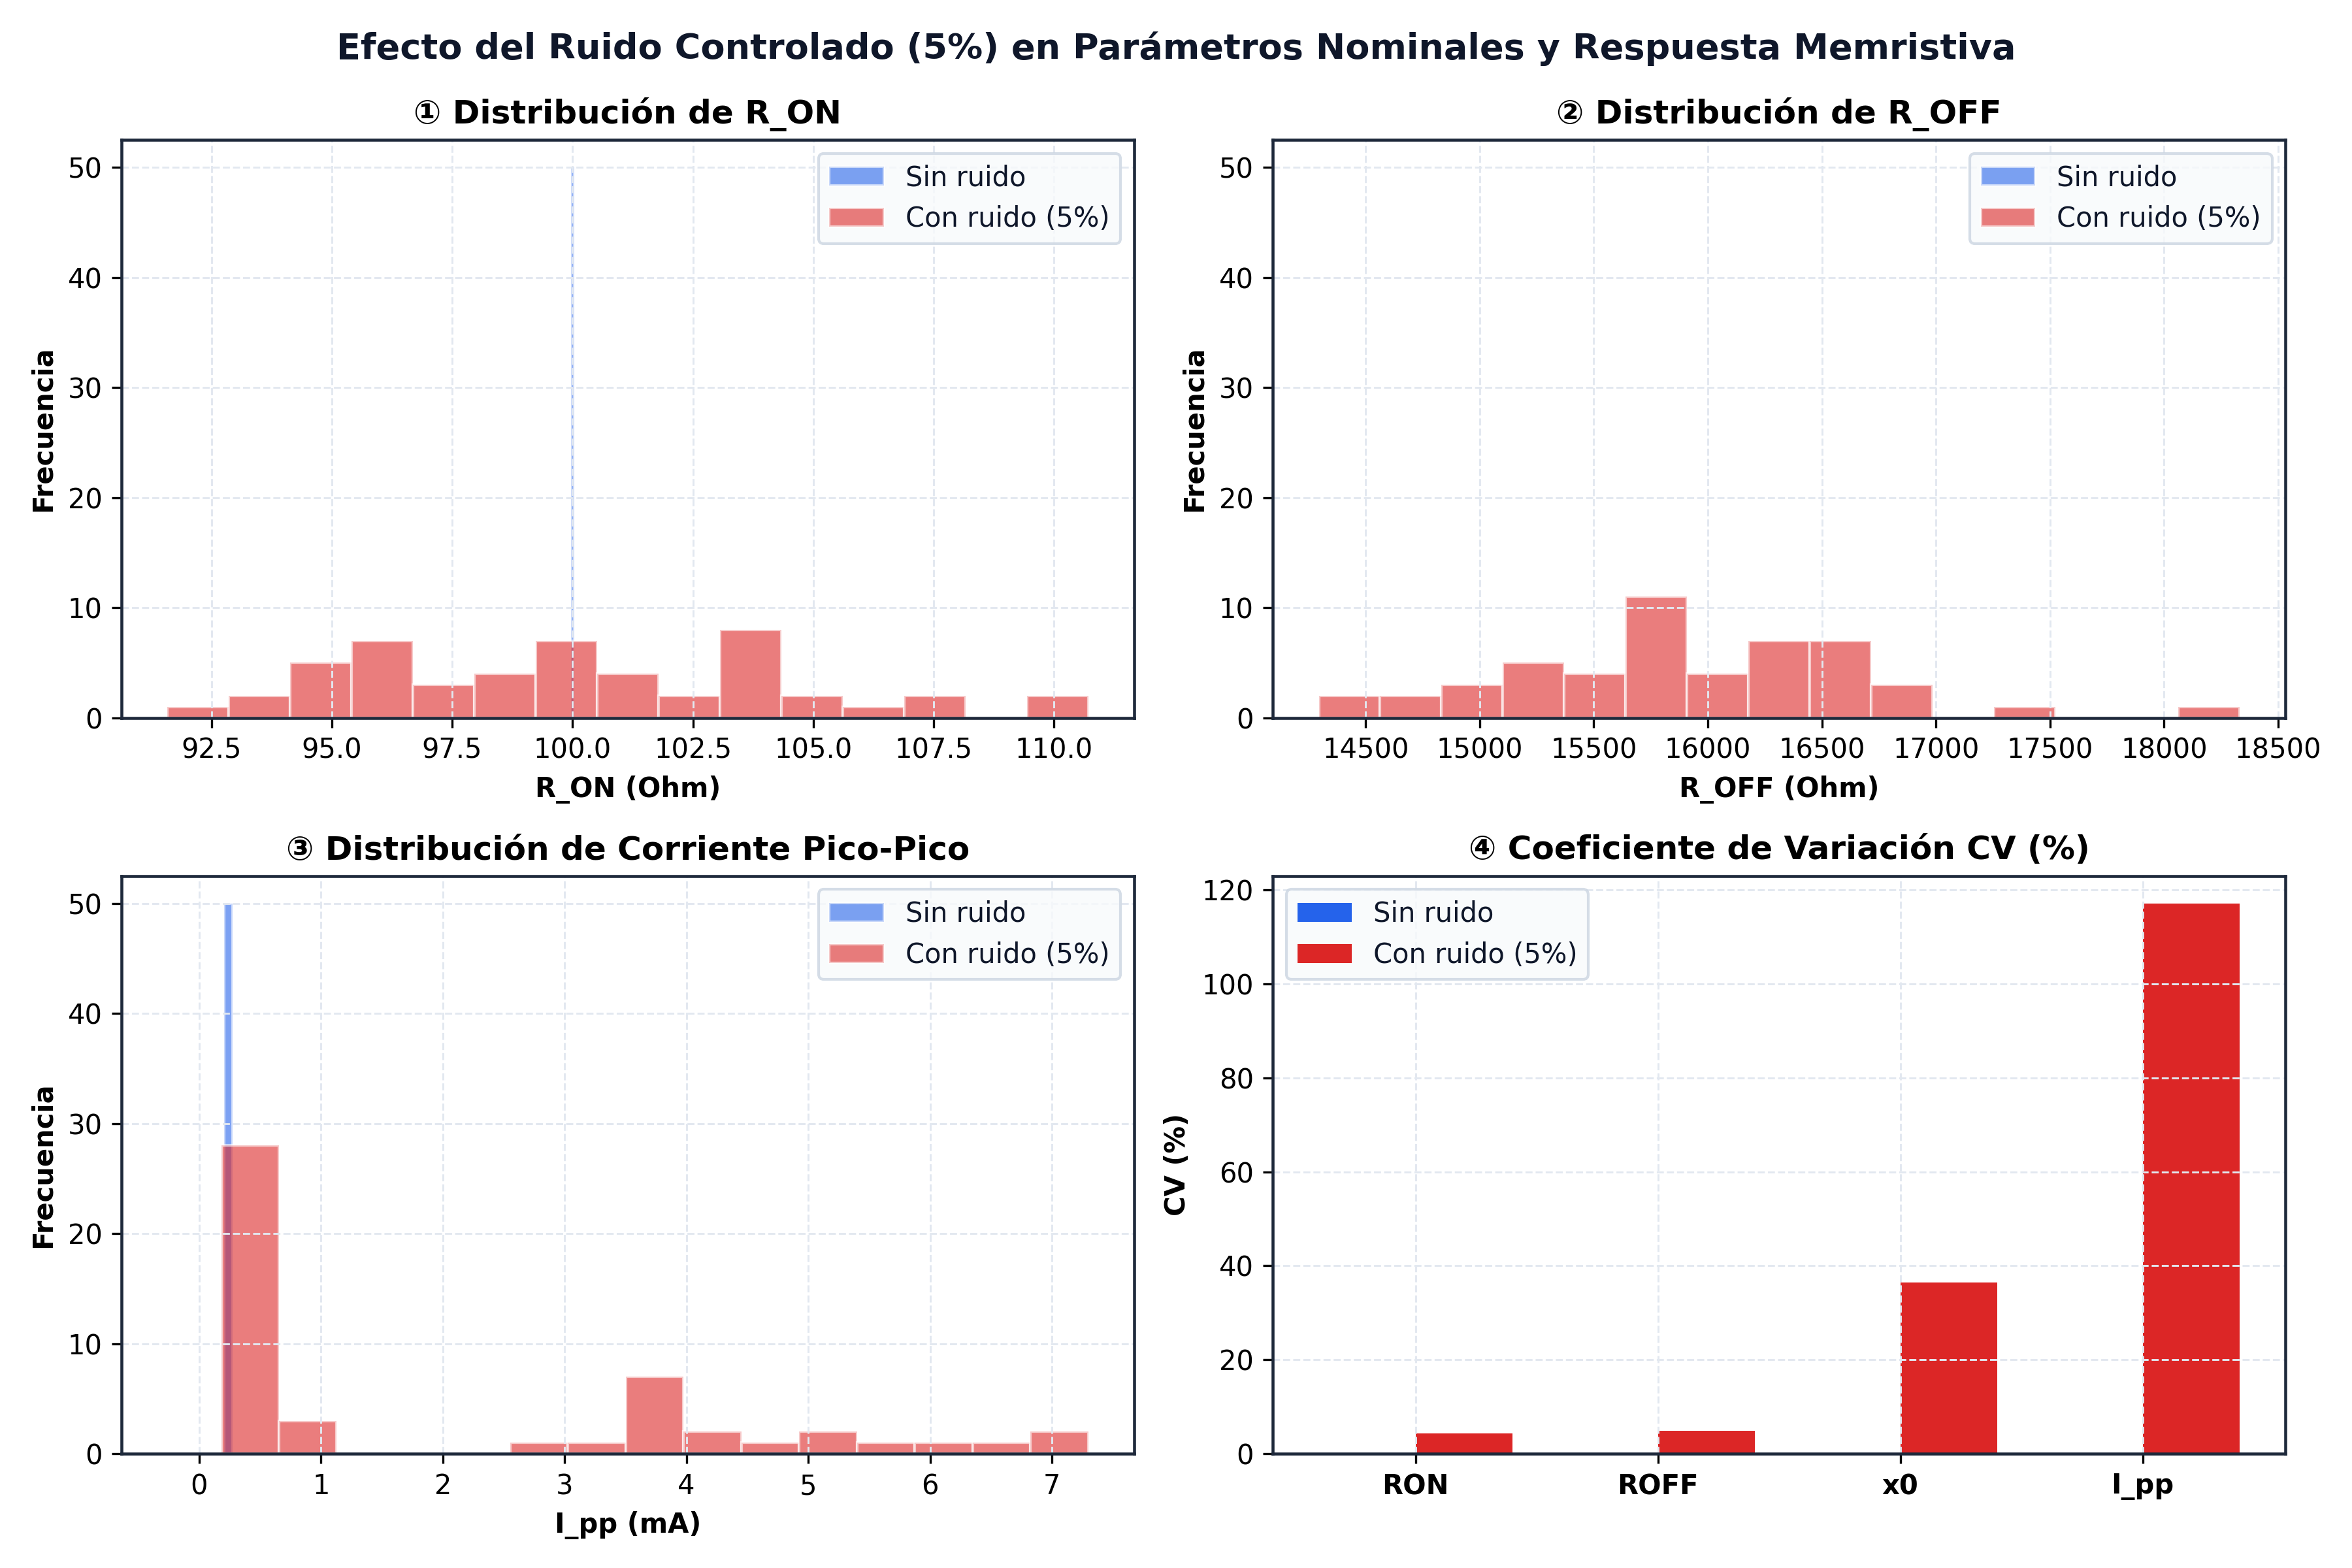
\includegraphics[width=0.7\textwidth]{figuras/fig_11_ruido.png}
    \caption{Sensibilidad del dispositivo a perturbaciones gaussianas del $5\%$ en sus parámetros nominales.}
    \label{fig:11_ruido}
\end{figure}

\textbf{Propósito y Relevancia:} La figura compara las distribuciones de $R_{\mathrm{ON}}$, $R_{\mathrm{OFF}}$ y corriente pico a pico, además del coeficiente de variación, entre dispositivos nominales y dispositivos con perturbaciones paramétricas. No representa una respuesta frecuencial ni permite concluir que el estado del memristor actúe como filtro pasa-bajos.

\begin{figure}[H]
    \centering
    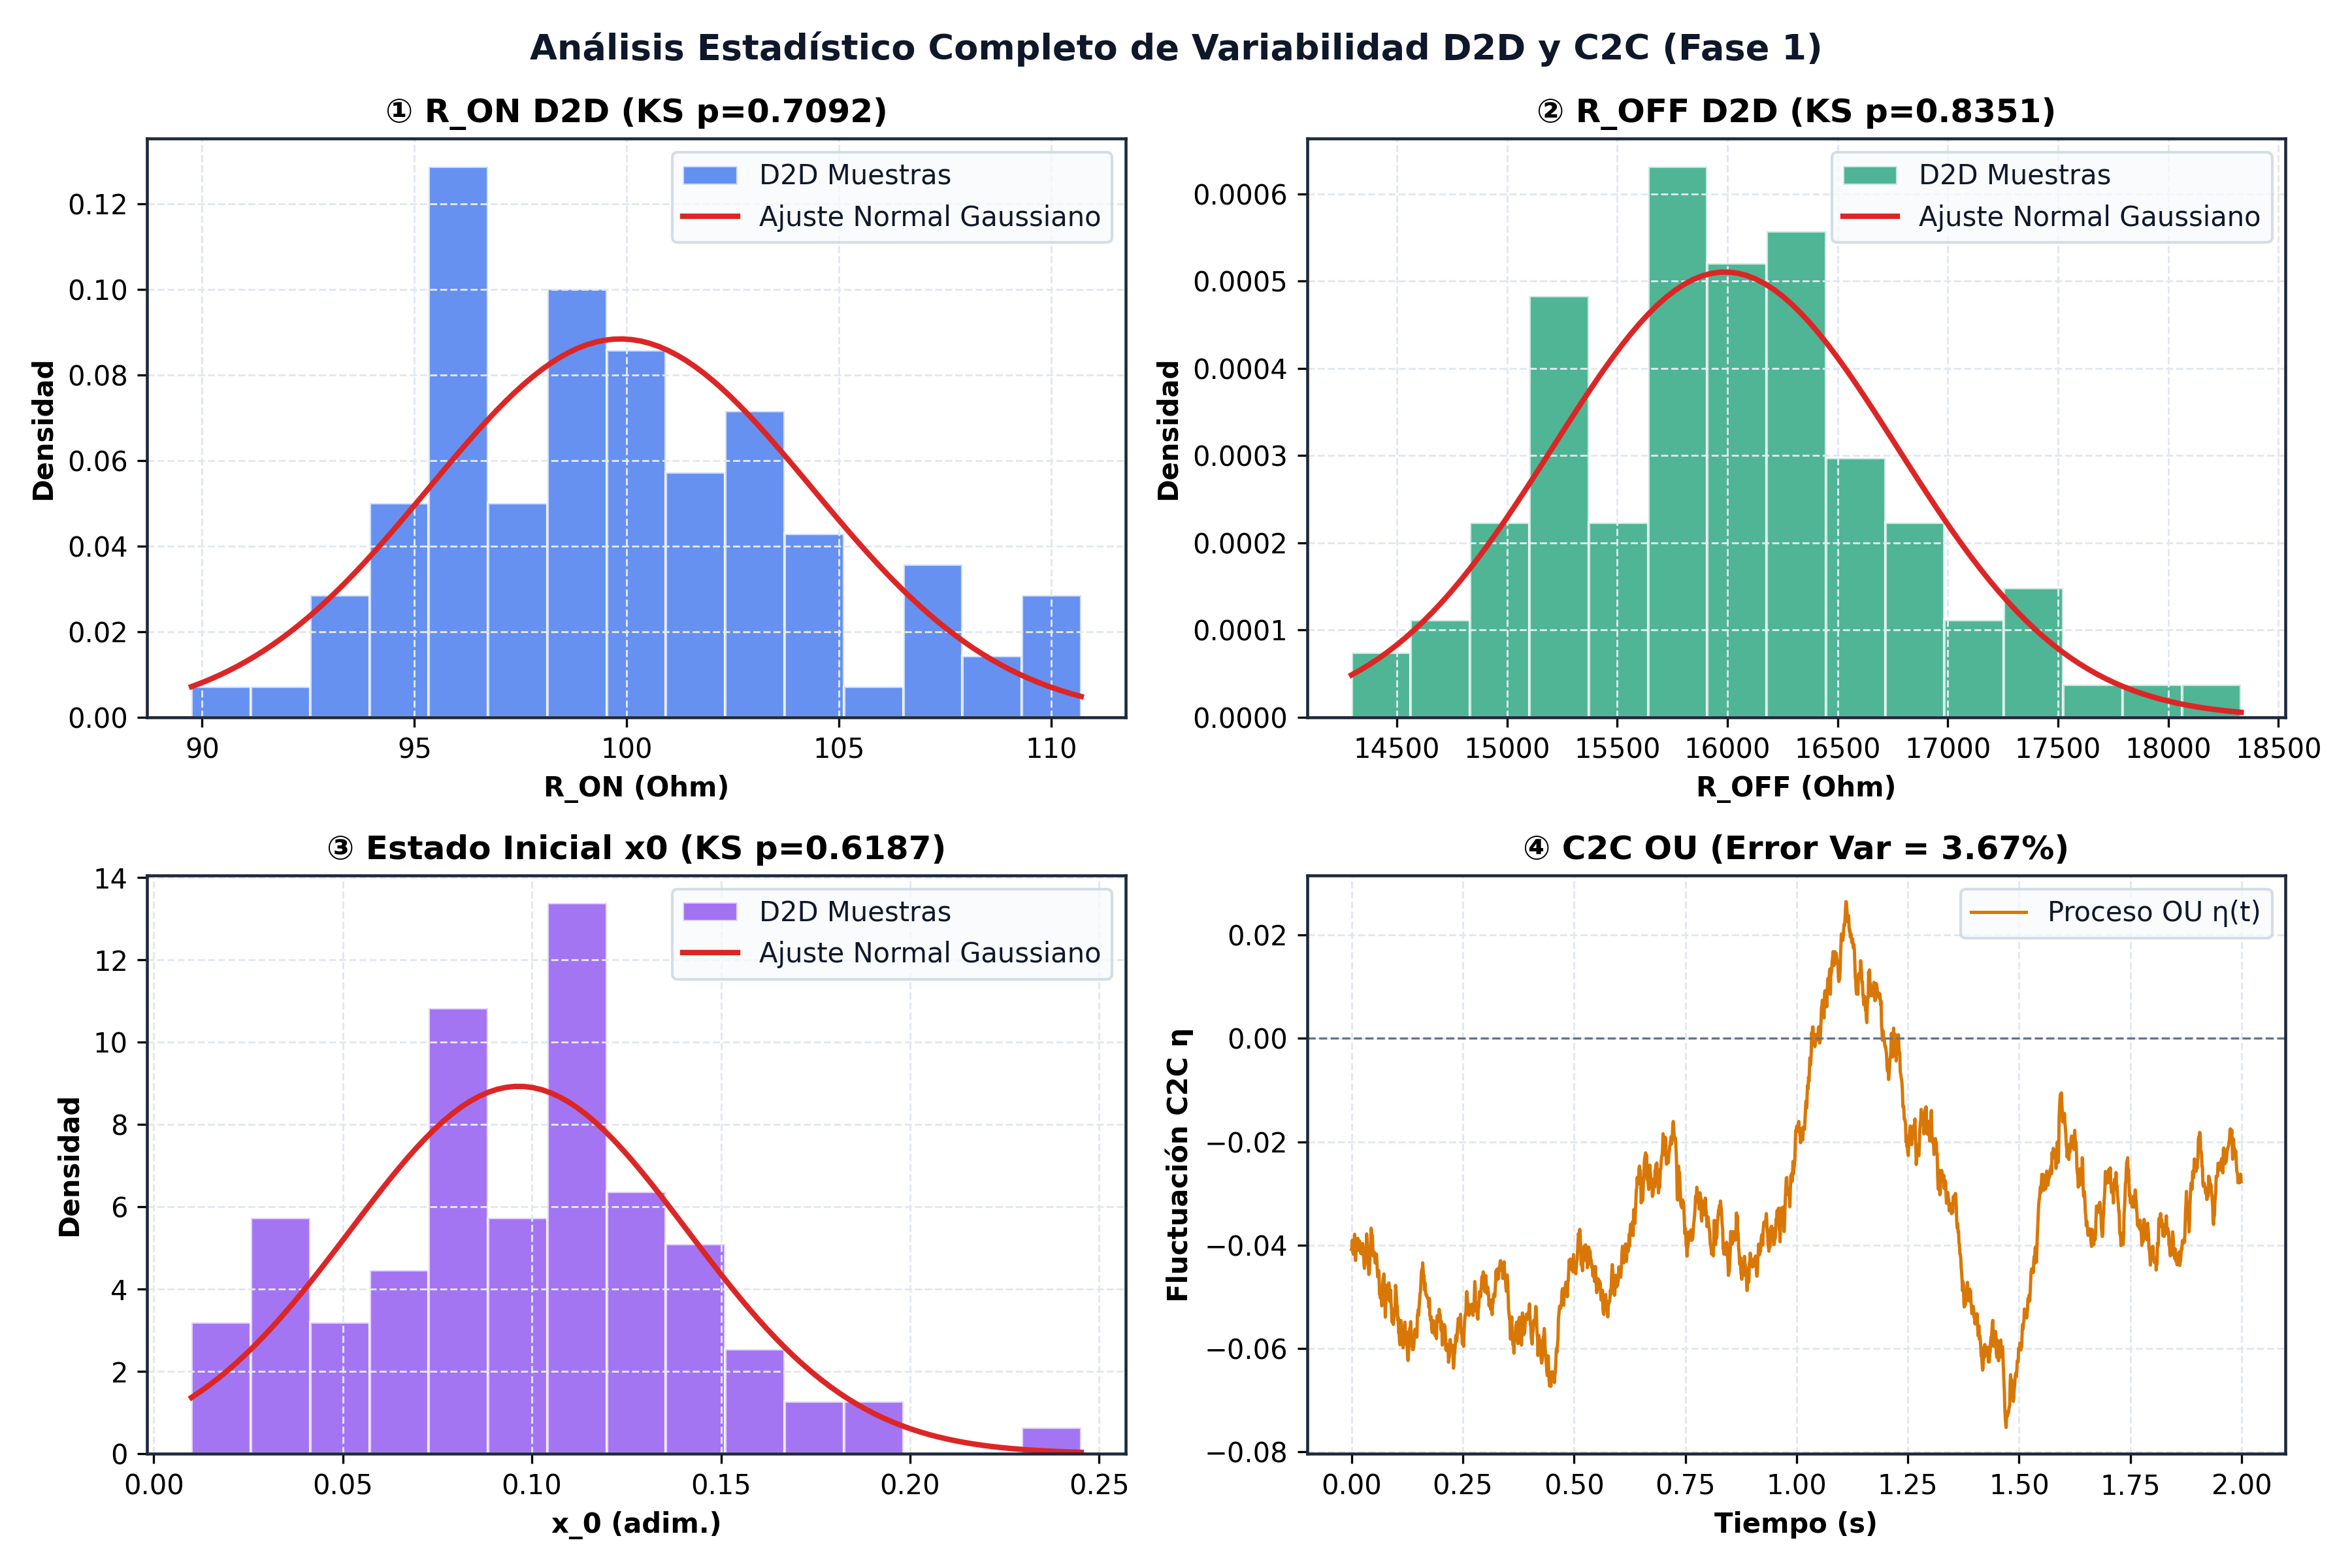
\includegraphics[width=0.8\textwidth]{figuras/fig_12_estadistica.png}
    \caption[Estadística D2D reportada]{Distribuciones D2D y pruebas KS de una corrida archivada distinta del cálculo reproducido con \texttt{05\_d2d\_c2c.py}.}
    \label{fig:12_estadistica}
\end{figure}

Los valores $p$ del panel, incluido $0.7092$ para $R_{\mathrm{ON}}$, proceden de la corrida archivada en \texttt{validacion\_estadistica\_completa.csv}, generada por \texttt{12\_estadistica.py}. Esa rutina usa una muestra distinta y ajusta media y desviación muestrales; no se revalidó la calibración del KS tras estimar esos parámetros con la misma muestra. El valor $0.8959$ informado arriba proviene de \texttt{05\_d2d\_c2c.py}, con los valores nominales para normalizar y contrastar contra $\mathcal{N}(0,1)$. Son análisis diferentes, por lo que sus $p$-valores no son intercambiables; el análisis archivado no se reprodujo en esta revisión.

\textbf{Propósito y Relevancia:} El panel reúne resúmenes estadísticos de muestras simuladas. Estos histogramas describen la población generada por el modelo; no demuestran que esa población reproduzca una distribución experimental ni validan arreglos físicos.

% =====================================================================
% Marco Práctico --- Sección 3.7: Fase 2
% =====================================================================

\subsection{Etapa 2 --- Neuronas Spiking y Sistema Híbrido}
\label{ch:fase2}

En esta segunda fase, el proyecto integra matemáticamente el modelo de neurona biológica Leaky Integrate-and-Fire (LIF) junto con el dispositivo memristivo, creando el primer bloque de construcción analógico (Memristor--Neurona) capaz de emular codificación temporal y procesamiento neuromórfico sensorial.

% =====================================================================
\subsubsection{Etapa 2.1: Neurona LIF y Acoplamiento Híbrido}
\label{sec:etapa2_1}

\paragraph{Implementación Cualitativa y Teoría Física}
El circuito híbrido simulado conecta un modelo de memristor en serie entre un estímulo de entrada (voltaje sensorial o pre-sináptico) y una neurona LIF. El potencial de membrana se representa como el voltaje de un capacitor $V_C(t)$ sujeto a una corriente de fuga paralela $R_{\mathrm{leak}}$; no se trata de un circuito físico medido.

La ecuación diferencial estocástica que rige el potencial de membrana está dada por:
\begin{equation}
C_m \frac{dV_C}{dt} = -\frac{V_C(t) - V_{\mathrm{rest}}}{R_{\mathrm{leak}}} + I_{\mathrm{inj}}(t) + \sigma_n \cdot \eta(t)
\label{eq:lif_hibrida}
\end{equation}

El acoplamiento se logra inyectando la corriente transmembrana $I_{\mathrm{inj}}(t)$, cuyo valor es dictaminado por la ley de Ohm en la rama de entrada a través de la conductancia del memristor dependiente del estado:
\begin{equation}
I_{\mathrm{inj}}(t) = \frac{V_{\mathrm{in}}(t) - V_C(t)}{R_S(x(t))}
\label{eq:i_inyectada}
\end{equation}

Cuando $V_C(t) \geq V_{\mathrm{th}}$, la neurona genera matemáticamente un evento discreto (\textit{spike}), y resetea instantáneamente su potencial a $V_{\mathrm{reset}}$, entrando en un período refractario absoluto.

Para representar un \textit{sensor volátil}, se emplea un modelo computacional inspirado en dióxido de hafnio (HfO$_2$). Incluye un término fenomenológico de relajación del estado en ausencia de estímulo:
\begin{equation}
\frac{dx}{dt} = f(V_M, x) - \frac{x}{\tau_{\mathrm{relax}}} \left(1 - H(V_M - V_{\mathrm{hold}})\right)
\label{eq:hfo2_dinamica}
\end{equation}

Cualitativamente (Figura~\ref{fig:hfo2_isi_hibrido}), en la simulación el estímulo de $1.5\,\mathrm{V}$ cambia el estado y la resistencia del modelo memristivo, modificando la corriente de entrada y los intervalos entre disparos. La figura ilustra adaptación temporal dentro de este modelo; no demuestra transducción biológica ni una respuesta de un dispositivo fabricado.

\begin{figure}[H]
    \centering
    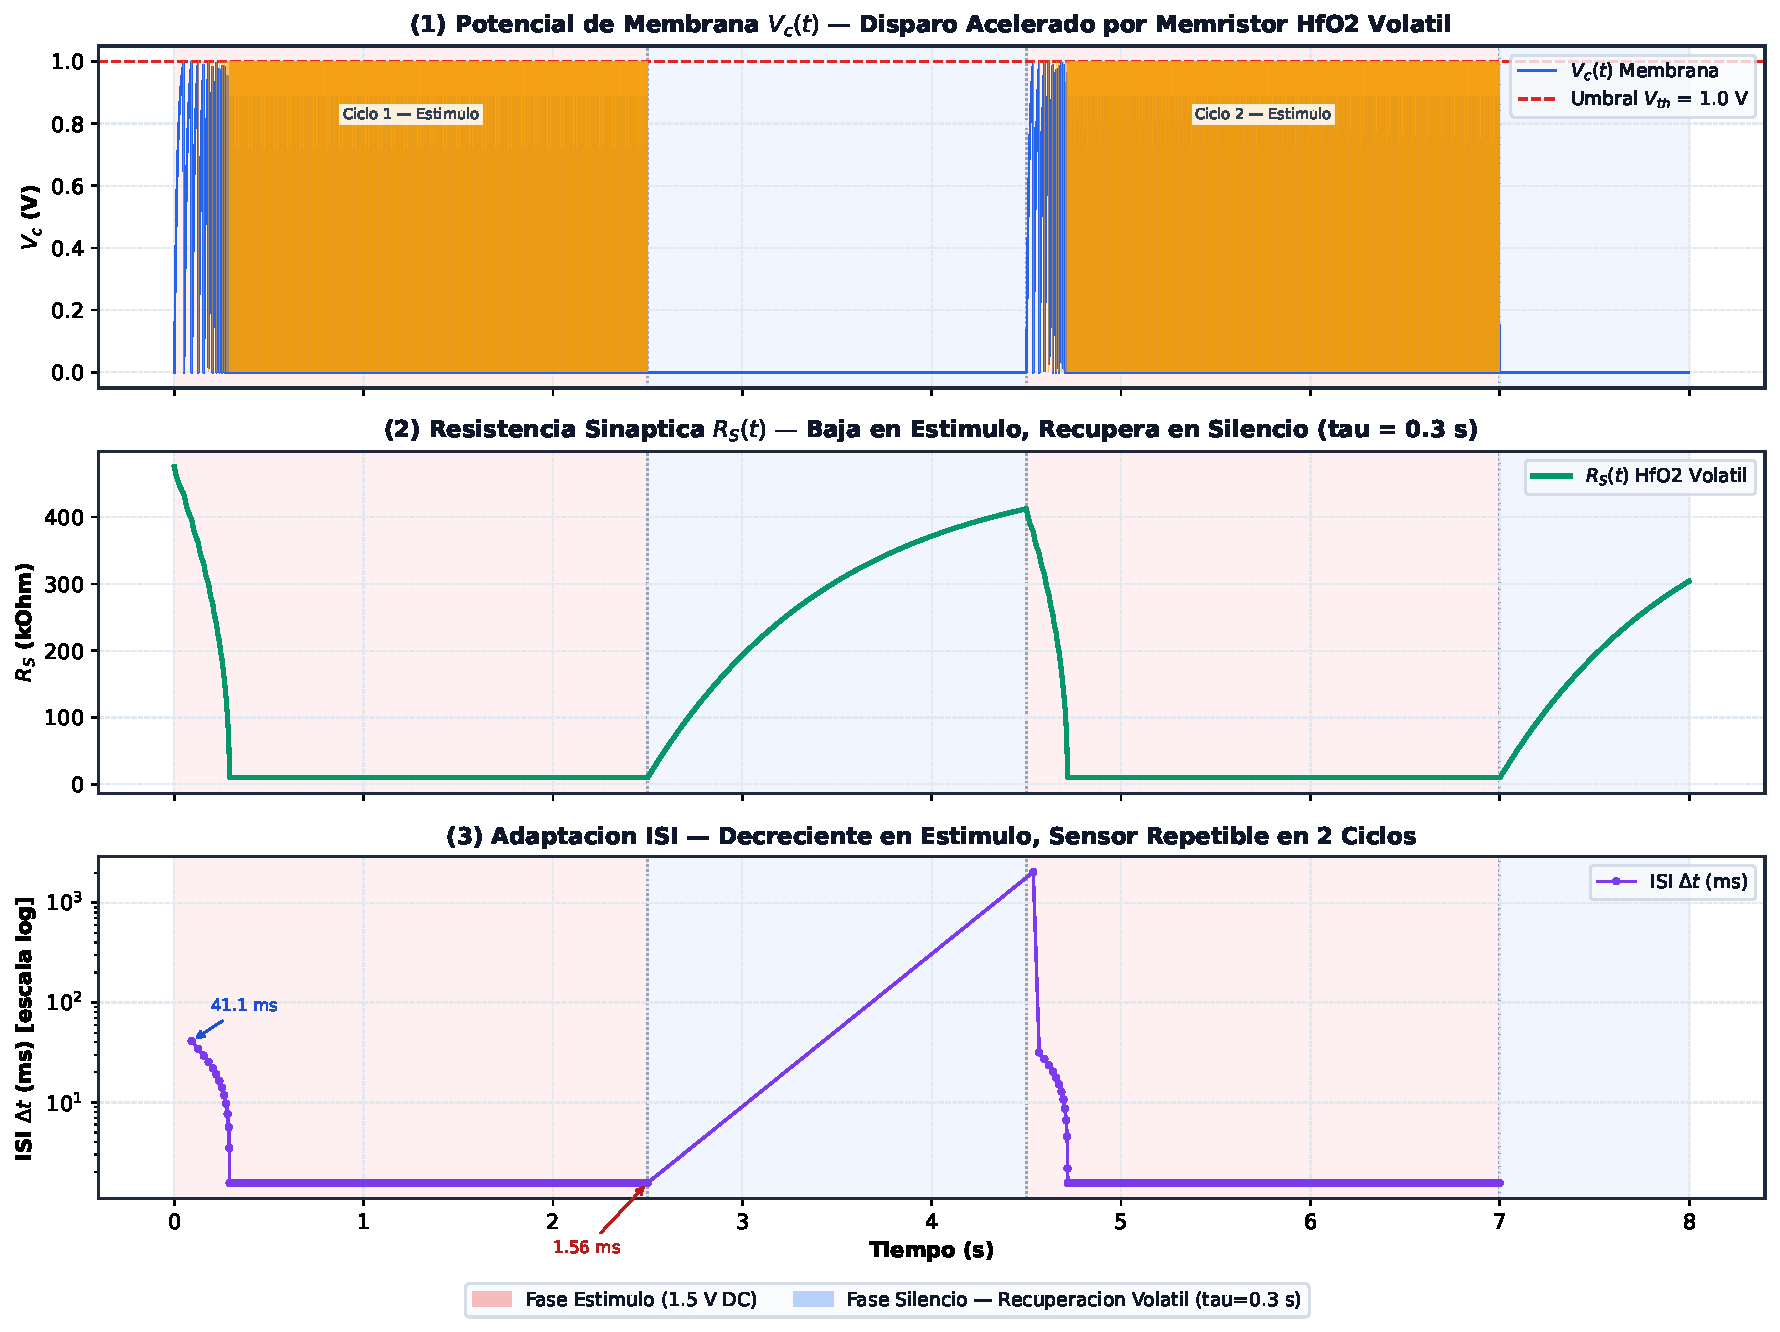
\includegraphics[width=0.85\textwidth]{figuras/fig_06_hfo2_isi_legible.pdf}
    \caption{Respuesta cualitativa del sistema híbrido: Potencial de membrana $V_C(t)$ evidenciando la aceleración temporal (top), Resistencia $R_S(t)$ descendente (centro), e Intervalo Inter-Spike (ISI) modularizado (abajo).}
    \label{fig:hfo2_isi_hibrido}
\end{figure}

\textbf{Propósito y Relevancia:} La figura ilustra el acoplamiento implementado entre el modelo memristivo y la neurona LIF. No constituye una validación de un sensor físico ni de un receptor nociceptivo.

\paragraph{Validación Cuantitativa Computacional}
La integridad matemática de esta fase fue comprobada contra soluciones exactas y papers de referencia del estado del arte.

\begin{figure}[H]
    \centering
    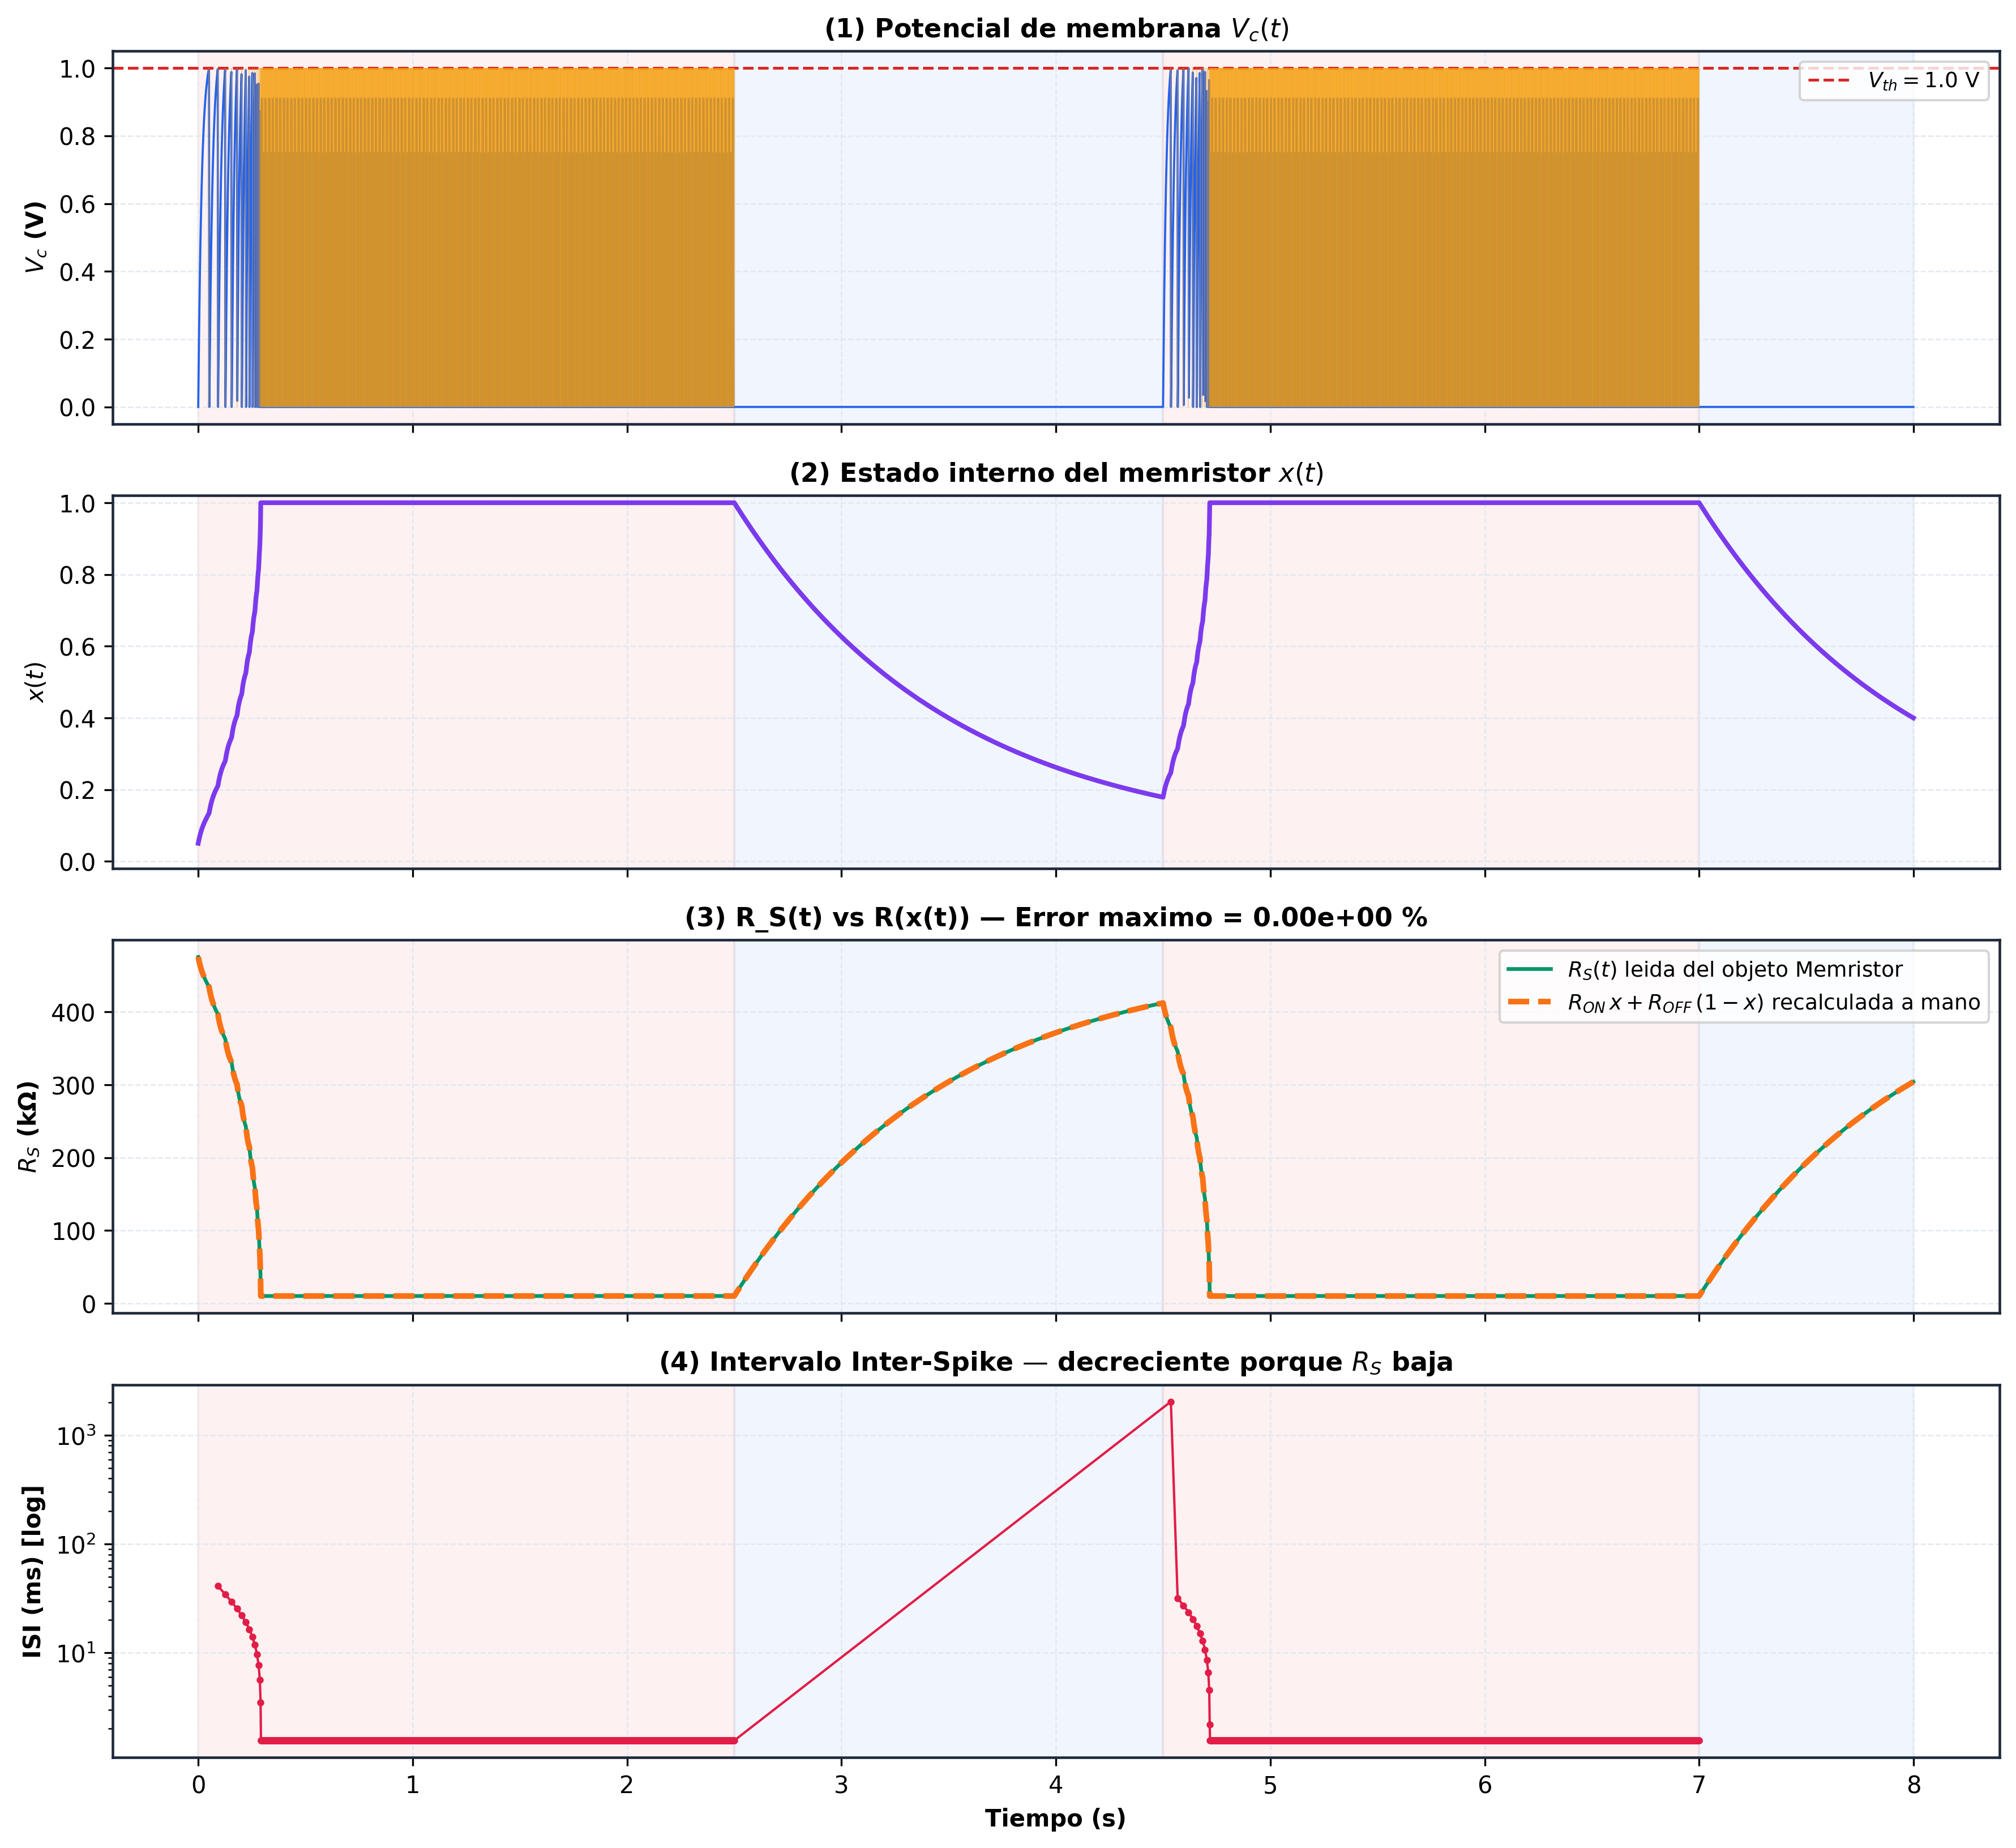
\includegraphics[width=0.7\textwidth]{figuras/fig_08_rs_x.png}
    \caption{Verificación de la resistencia en serie $R_S$ proveniente de la dinámica de acoplamiento de $x$.}
    \label{fig:08_rs_x}
\end{figure}

\textbf{Propósito y Relevancia:} Este gráfico comprueba, para la ejecución y las variables mostradas, la consistencia entre $R_S$ y $x(t)$ según la relación implementada. No prueba por sí solo ausencia general de pérdida de eventos, retrasos ni errores en todas las ejecuciones.

\textbf{Solución Analítica LIF Subumbral:}
Se sometió el módulo integrador numérico de la neurona LIF a una validación estricta frente a su solución analítica exacta de circuito RC subumbral:
\begin{equation}
V_m(t) = V_{\infty} + (V_{m,0} - V_{\infty}) e^{-t/\tau_{eq}}
\end{equation}
La comparación cuantitativa entre la simulación discreta y la solución RC analítica es distinta de la comparación cualitativa con Wang descrita más adelante. En el CSV archivado \texttt{lif\_rc\_validation.csv}, el cálculo de $R^2$ sobre las 1000 muestras disponibles es $0.9999815$, que redondeado a cuatro decimales da $1.0000$. Este resultado describe solo esa prueba subumbral y no se atribuye a la comparación cualitativa ni demuestra exactitud general del integrador para otros pasos o condiciones.

\begin{figure}[H]
    \centering
    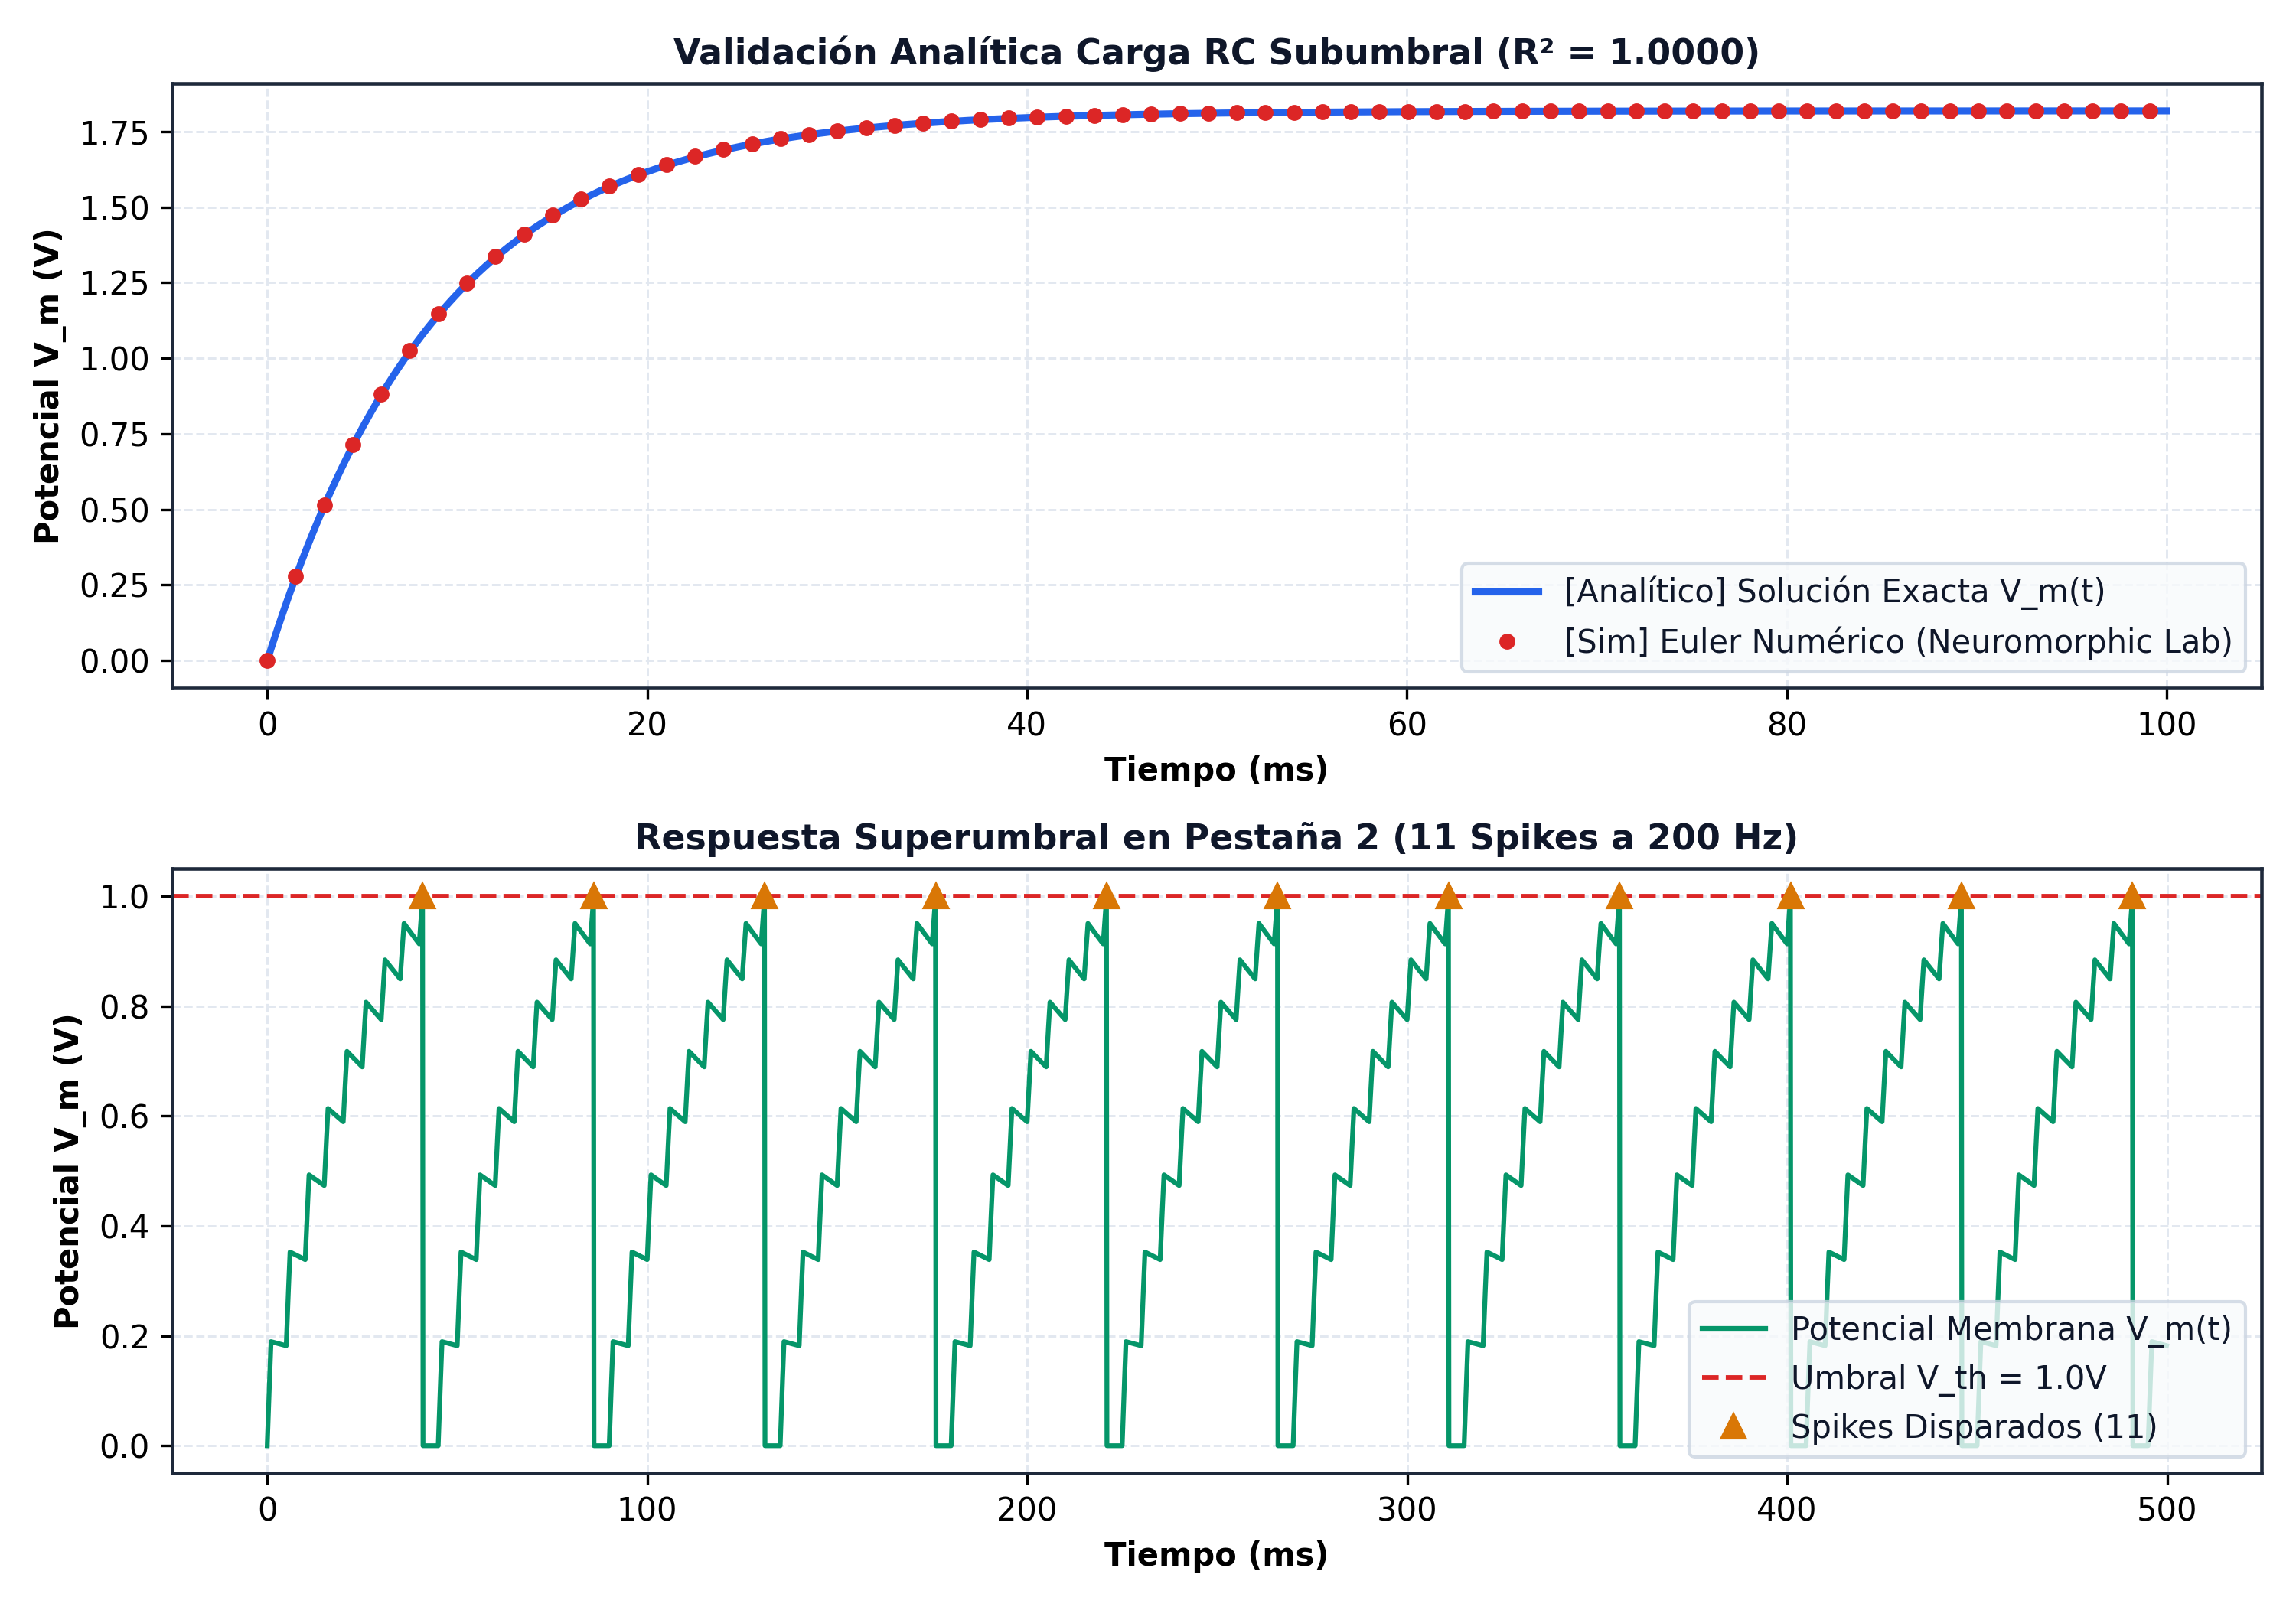
\includegraphics[width=0.85\textwidth]{figuras/fig_03_lif.png}
    \caption{Validación analítica subumbral de la neurona LIF frente a la solución RC exacta en respuesta al impulso.}
    \label{fig:val-lif}
\end{figure}

\textbf{Propósito y Relevancia:} La comparación permite evaluar la respuesta subumbral para las condiciones ensayadas. El valor archivado no basta para descartar sesgos algorítmicos en otras configuraciones ni para afirmar que el núcleo esté libre de errores.

\textbf{Comportamiento cualitativo de integración y disparo LIF:}
La neurona LIF del simulador comparte el comportamiento funcional descrito por Wang et al.~\cite{2}: integra los estímulos, alcanza el umbral y genera eventos de disparo con reinicio. La Figura~\ref{fig:lif-behavior-wang} muestra esta secuencia en el simulador \texttt{Neuromorphic Lab}, con la configuración guardada en \url{02_SOFTWARE/neuromorphic_lab/configs/lif_config.json}: $C_m=100\,\mathrm{nF}$, $R_S=100\,\mathrm{k\Omega}$, $R_{\mathrm{leak}}=1\,\mathrm{M\Omega}$, umbral de $1\,\mathrm{V}$ y período refractario de $2\,\mathrm{ms}$. La entrada simulada es un tren unipolar de $2\,\mathrm{V}$ a $200\,\mathrm{Hz}$, con ciclo útil del $20\%$, durante $0.5\,\mathrm{s}$. Con paso de integración de $1\,\mathrm{\mu s}$, esta ejecución produce 11 eventos de disparo.

\begin{figure}[H]
    \centering
    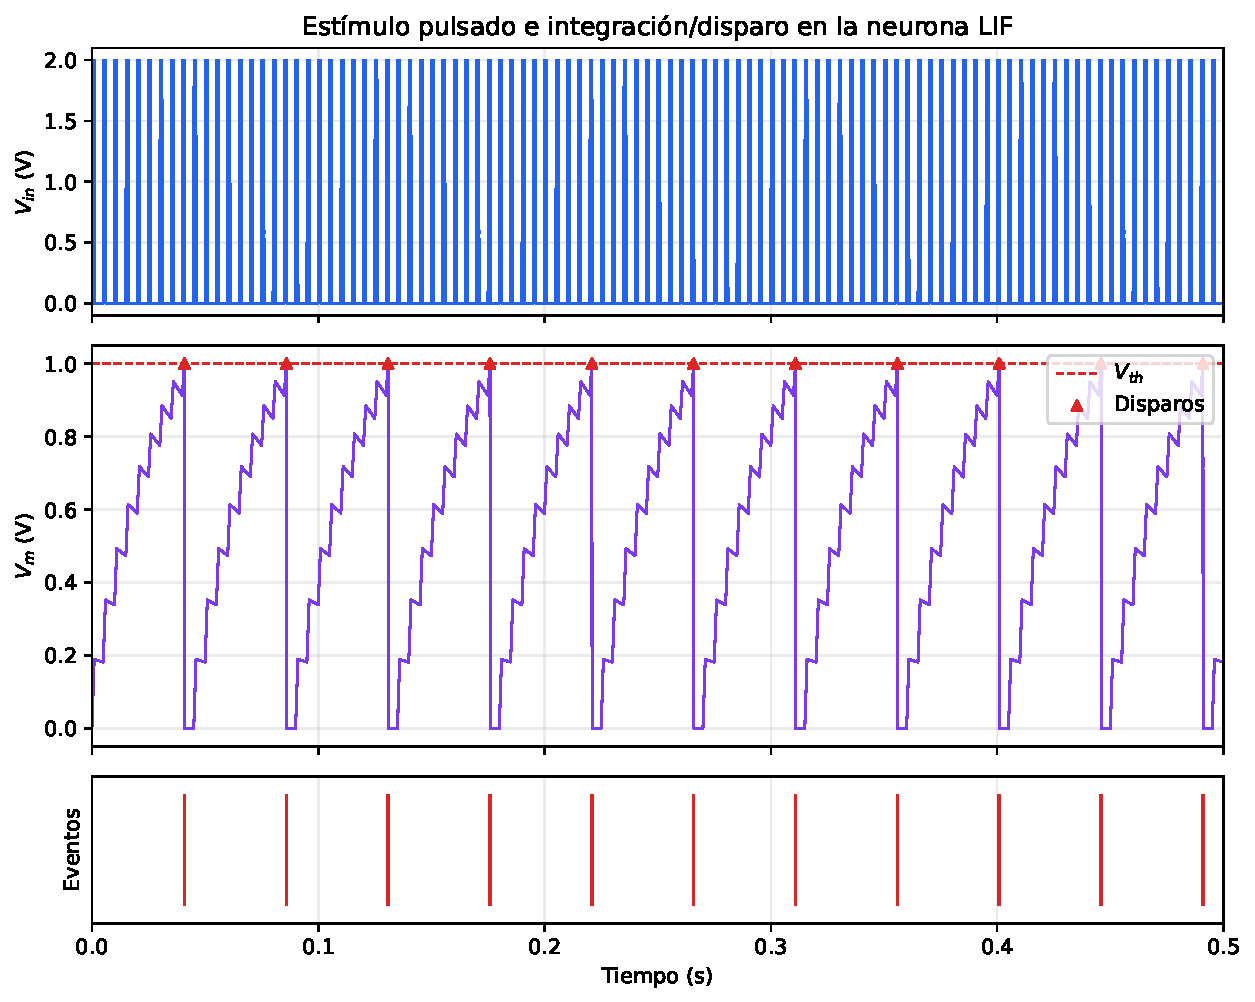
\includegraphics[width=0.95\textwidth]{figuras/fig_13_lif_behavior.pdf}
    \caption[Respuesta de la neurona LIF]{Respuesta de la neurona LIF del simulador: estímulo pulsado, integración del potencial de membrana y eventos de disparo, en concordancia funcional con la dinámica descrita por Wang et al.~\cite{2}.}
    \label{fig:lif-behavior-wang}
\end{figure}

\textbf{Propósito y Relevancia:} La figura documenta que el simulador LIF implementa la secuencia de integración y disparo. El panel inferior es un raster de eventos, no una forma de onda de voltaje de salida ni una medición física.

% =====================================================================
% Marco Práctico --- Sección 3.8: Fase 3
% =====================================================================

\subsection{Etapa 3 --- Plasticidad Sináptica}
\label{ch:fase3}

Esta fase describe simulaciones de plasticidad LTP/LTD y STDP con modelos
memristivos. Las comparaciones con Jo et al. (2010) se recalcularon con
el protocolo y las particiones descritos abajo, usando puntos
digitalizados de las figuras publicadas. No son mediciones propias ni
certifican por sí solas una respuesta física.

% =====================================================================
\subsubsection{Etapa 3.1: LTP/LTD y STDP}
\label{sec:etapa3_1}

\paragraph{Implementación Cualitativa (LTP/LTD)}
Para estudiar la respuesta acumulativa de la conductancia sináptica (representando el peso lógico $W_{ij}$), se aplicaron secuencias controladas de trenes de pulsos de voltaje idénticos. Matemáticamente, cada pulso induce un minúsculo diferencial $dx$ positivo o negativo sobre el estado del filamento según su polaridad. 

Los pulsos positivos inducen la Potenciación a Largo Plazo (LTP), aumentando la conductancia de forma progresiva. Los pulsos negativos provocan la Depresión a Largo Plazo (LTD), borrando la historia almacenada. La Figura~\ref{fig:20_vi_ltp_ltd} documenta voltaje, corriente, resistencia y conductancia durante pulsos LTP/LTD; la curva temporal escalonada descrita en el informe previo no tiene una figura independiente incluida en este paquete.

El ajuste STDP y sus puntos reservados se muestran en la Figura~\ref{fig:stdp_curve_ch3} del Cap\'itulo~3. Se conserva aqu\'i la interpretaci\'on ampliada de la partici\'on y sus l\'imites.

\textbf{Propósito y Relevancia:} La figura documenta la asimetría del conjunto digitalizado y el error de predicción en los puntos reservados. No certifica la precisión de un cambio de conductancia físico ni la validez general del componente.

\textbf{Curva LTP/LTD atribuida a Jo et al.}
El CSV \texttt{jo2010\_ltp\_ltd.csv} contiene 87 puntos atribuidos por el
validador a la Fig.~2a; no son 200 registros experimentales brutos. Se
simularon 100 pulsos SET de $+3.2\,\mathrm{V}$ y 100 RESET de
$-2.8\,\mathrm{V}$, ambos de $300\,\mu\mathrm{s}$, con lecturas a
$1\,\mathrm{V}$. De los 87 puntos, dos quedan fuera del intervalo de
0--200 pulsos; los 85 restantes se separan, dentro de cada rama, en
bloques contiguos 60/20/20: 50 de entrenamiento, 17 de validación y 18
de test. Se ajustan $R_{\mathrm{on}}$, $R_{\mathrm{off}}$, el coeficiente
de deriva efectivo y $x_0$ solo con entrenamiento; validación selecciona
entre tres inicializaciones. No se aplica un reescalado min--max ni una
calibración afín posterior. En test se obtuvo
$R^2_{\mathrm{residual}}=0.73988$, MAE $=8.3491\,\mathrm{nA}$,
RMSE $=8.6181\,\mathrm{nA}$ y ERP $=31.23\%$. Por rama, el resultado es
deficiente: $R^2=-8.54$ en LTP ($n=10$) y $R^2=-829.99$ en LTD ($n=8$).
Pearson agregado es $r=0.99303$ ($r^2=0.98610$), pero este valor mide
covariación y no sustituye el $R^2_{\mathrm{residual}}$: la predicción
de LTP es constante, por lo que su correlación no está definida; en LTD
se obtiene $r=-0.22170$ ($r^2=0.04915$).
Los parámetros efectivos se ajustan a la misma curva digitalizada y no
son una caracterización independiente del dispositivo; la evidencia es
parcial y no demuestra predicción independiente ni validación completa
del artículo.

La comparaci\'on LTP/LTD y sus puntos reservados se muestran en la Figura~\ref{fig:ltp_ltd_curve_ch3} del Cap\'itulo~3; se conserva aqu\'i el an\'alisis cuantitativo por rama.

\textbf{Propósito y Relevancia:} La figura muestra la forma de la curva bajo la normalización declarada. No demuestra fidelidad física general ni identifica un mecanismo microscópico concreto.


\begin{figure}[H]
    \centering
    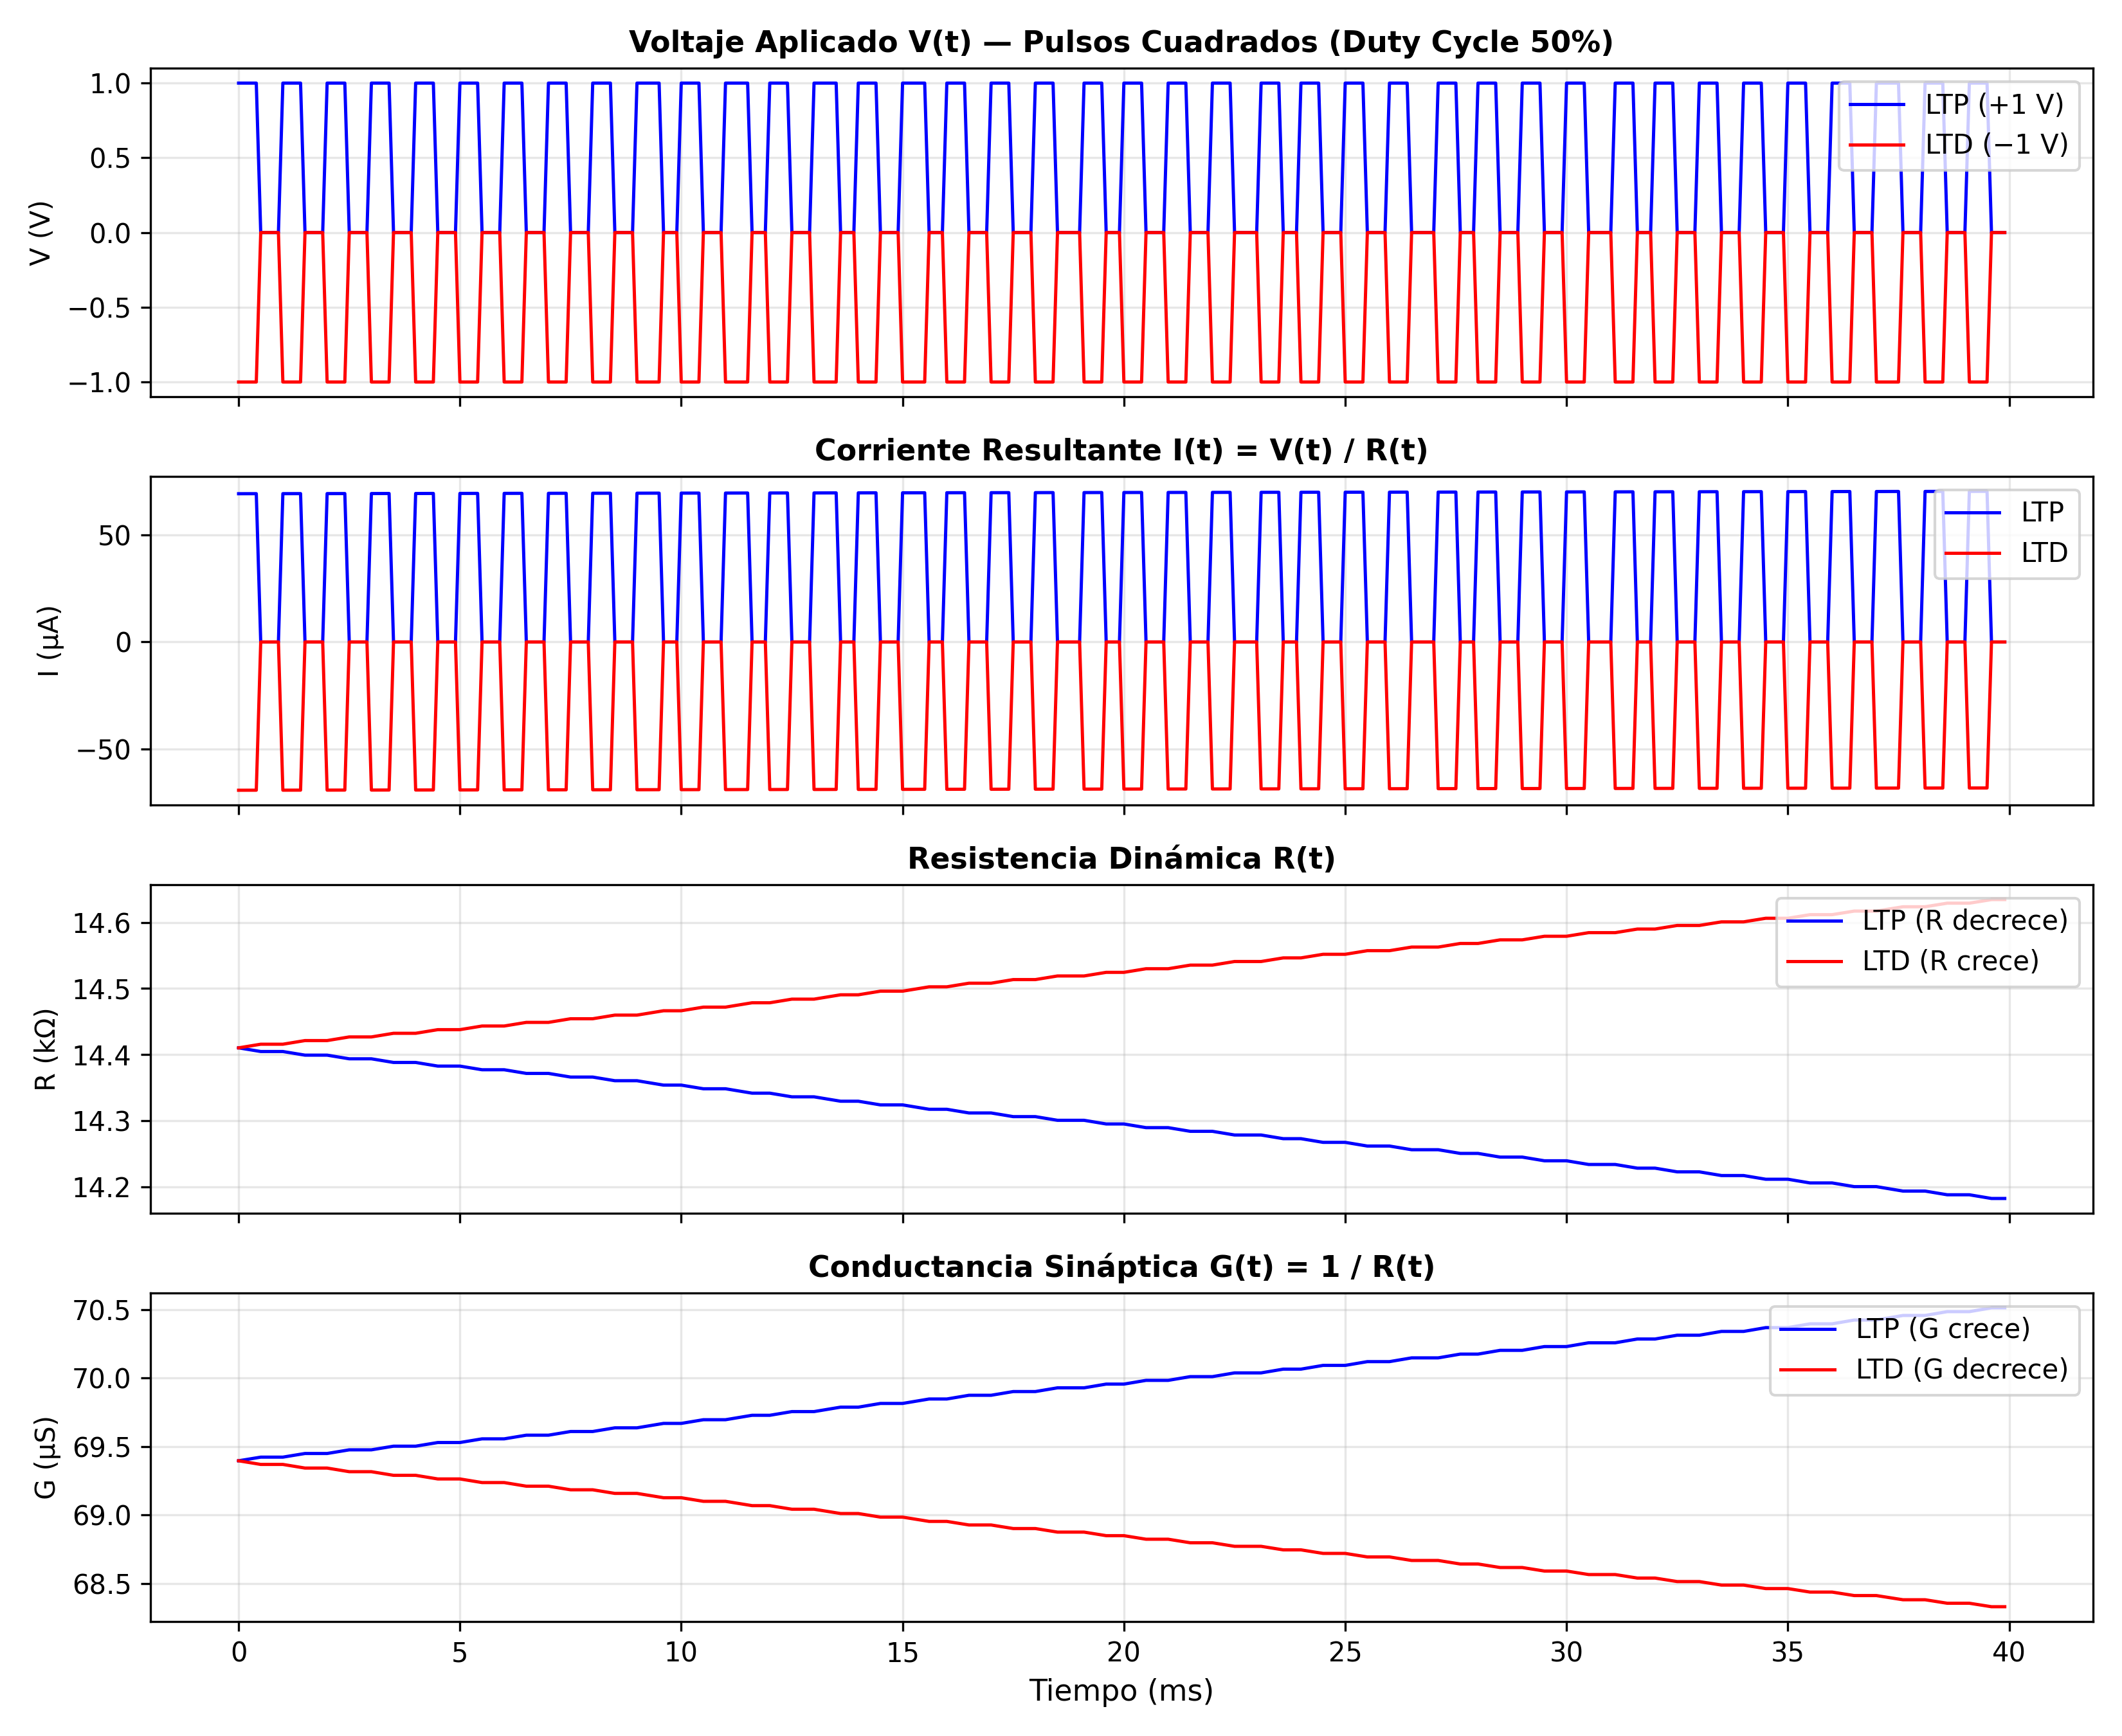
\includegraphics[width=0.7\textwidth]{figuras/fig_20_vi_ltp_ltd.png}
    \caption{Caracterización simultánea de voltaje, corriente, resistencia y conductancia durante pulsos LTP y LTD.}
    \label{fig:20_vi_ltp_ltd}
\end{figure}

\textbf{Propósito y Relevancia:} La figura muestra variables registradas por la simulación durante los pulsos. No constituye una observación microscópica ni una prueba general de conservación para otras configuraciones.

% =====================================================================
% Marco Práctico --- Sección 3.9: Etapa 4
% =====================================================================

\subsection{Etapa 4 --- Arquitecturas Matriciales y No Idealidades}
\label{ch:fase4}

La Etapa 4 estudia implementaciones a nivel de red mediante un
arreglo cruzado bidimensional (crossbar). Su aplicación al agente de
control se desarrolla en la subseccion siguiente. Los resultados
corresponden a modelos y entornos de simulación, no a mediciones de
un crossbar fabricado.

% =====================================================================
\subsubsection{Etapa 4.1: Matriz Crossbar e In-Memory}
\label{sec:etapa4_1}

Una matriz crossbar se representa por
$\mathbf{G}\in\mathbb{R}^{N\times M}$, con $N$ filas de entrada y
$M$ columnas de salida; cada intersección aloja un dispositivo
memristivo simulado.

En el modelo ideal, al aplicar un vector de voltajes de entrada
$\mathbf{V}=[V_1,V_2,\dots,V_N]^{\mathsf T}\in\mathbb{R}^{N}$ a las
filas, las conductancias en paralelo realizan una multiplicación
matriz-vector. La corriente $I_j$ de cada columna sigue la ley de Ohm
y la ley de corrientes de Kirchhoff:

\begin{equation}
I_j(t) = \sum_{i=1}^N V_i(t) \cdot G_{ij}(t) \quad \implies \quad \mathbf{I} = \mathbf{G}^{\mathsf T} \mathbf{V},\qquad \mathbf{I}\in\mathbb{R}^{M}
\label{eq:vmm_law}
\end{equation}

En un arreglo analógico ideal, las contribuciones de las celdas se procesarían en paralelo. Esta descripción algebraica no demuestra latencia física constante ni complejidad computacional $\mathcal{O}(1)$ para el solver numérico: el costo de resolver el modelo MNA se trata por separado en el Experimento~9.

\paragraph{Implementación Cualitativa (Operación Analógica $1 \times 1$)}
Se implementó y se visualizó estructuralmente el sistema base modular probando una celda atómica unitaria que simula la interacción macro-escalar. 

Como se ilustra en las salidas de simulación (Figuras~\ref{fig:crossbar_1x1_completo}a-d), al suministrar la onda cuadrada de voltaje al modelo, la dinámica de la celda memristiva de Yakopcic cambia su estado. La línea de columna calcula $\mathbf{I}=\mathbf{G}^{\mathsf T}\mathbf{V}$ en el modelo, con las filas de $\mathbf{G}$ asociadas a las entradas y las columnas a las salidas. Estas figuras ilustran la operación implementada; no son mediciones de hardware ni prueban por sí solas su comportamiento físico.

\begin{figure}[H]
    \centering
    \begin{subfigure}[b]{0.84\textwidth}
        \centering
        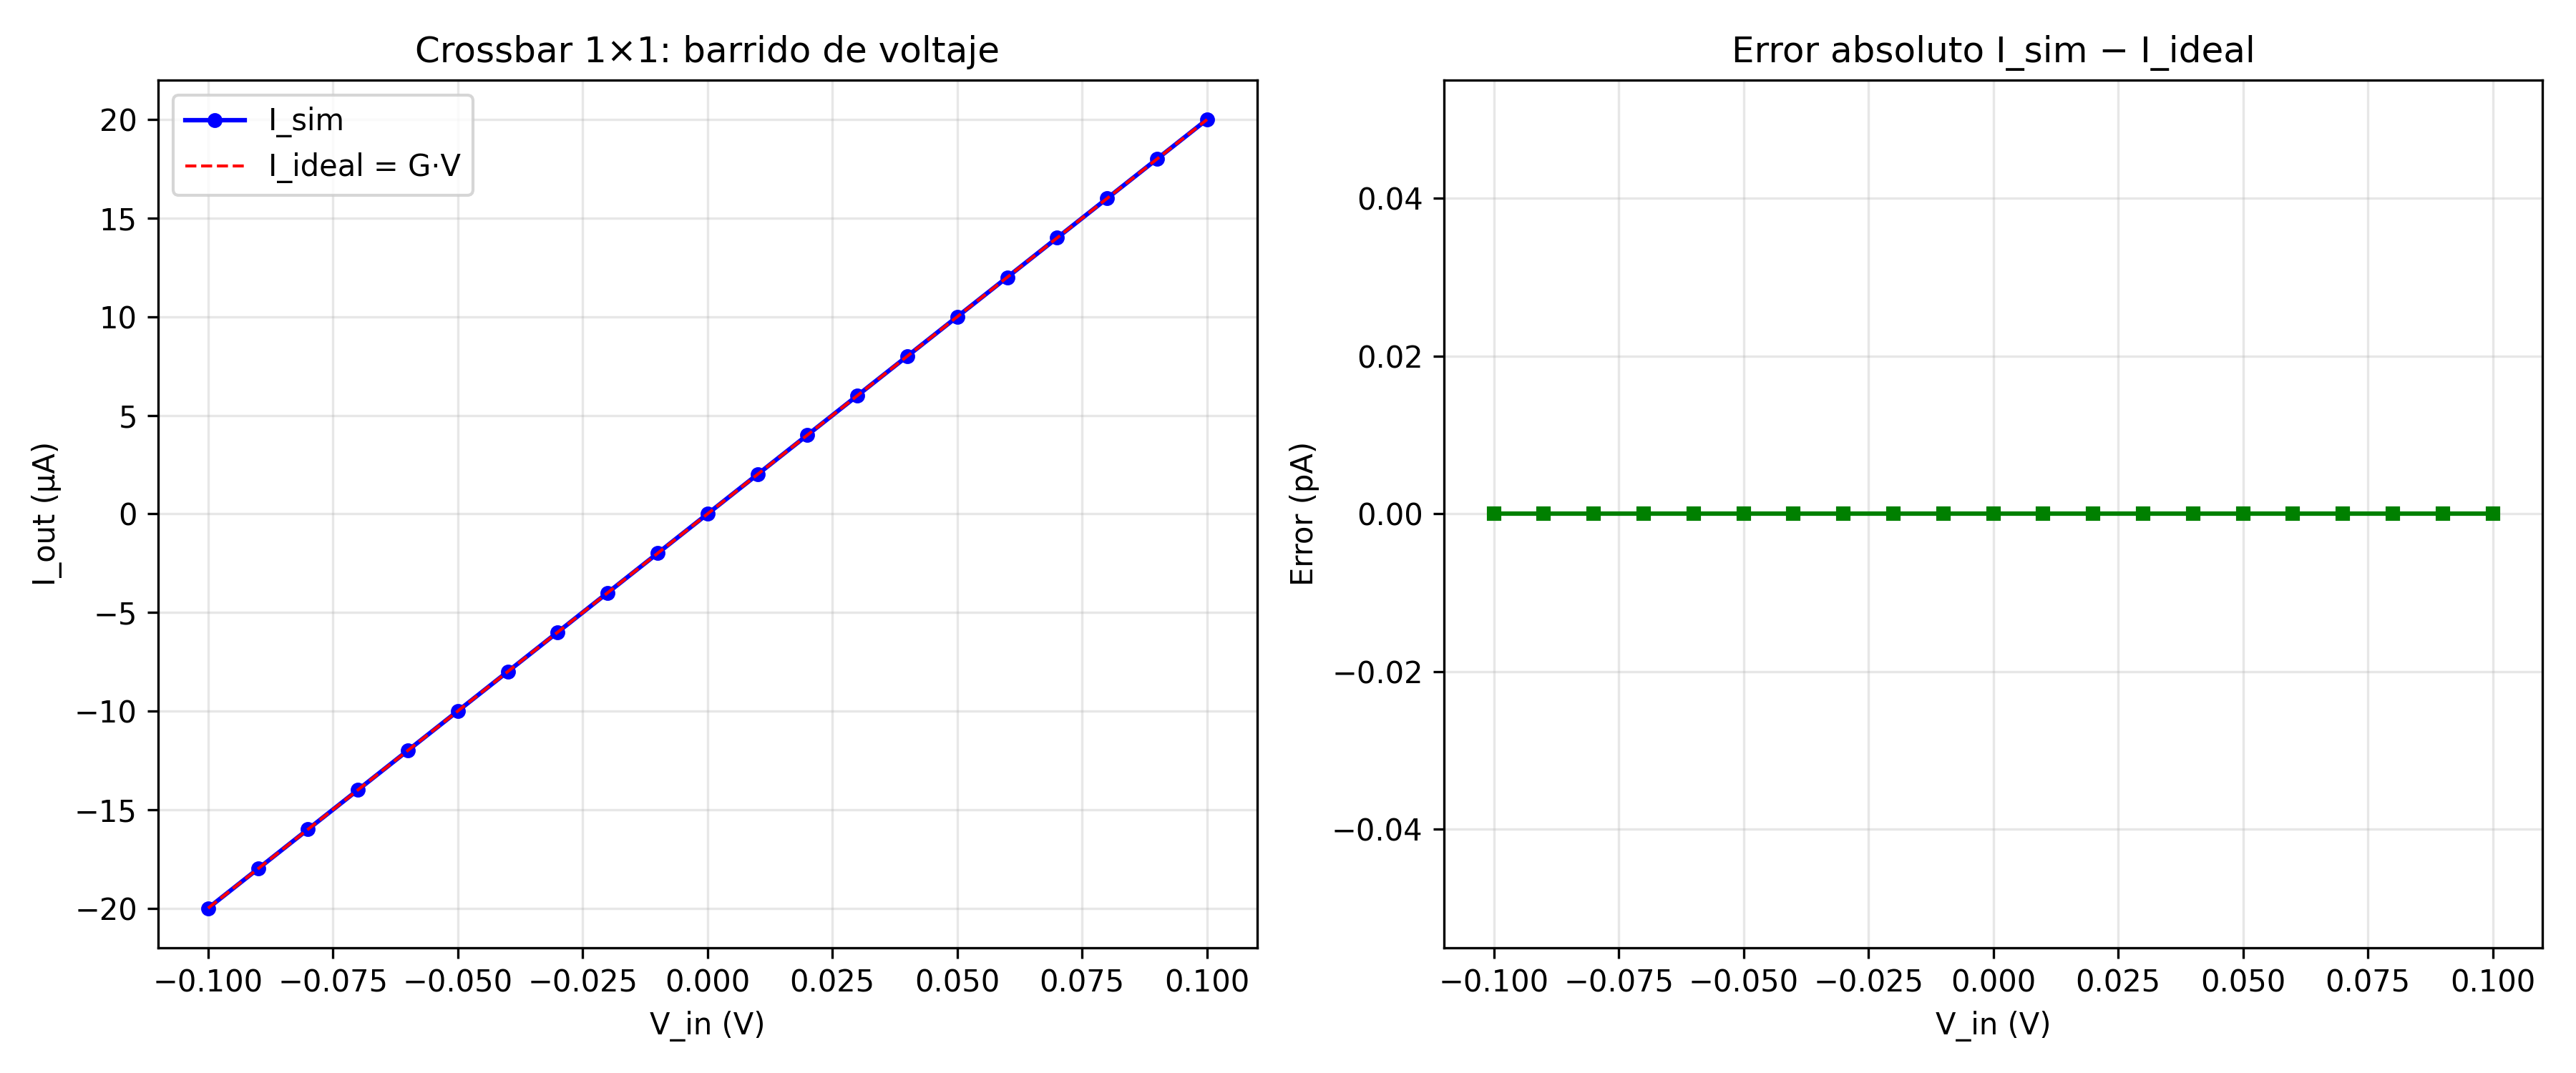
\includegraphics[width=\textwidth]{figuras/fig_21a_crossbar_V.png}
        \caption{Pulsos de excitación por línea de Palabra $V_i(t)$.}
    \end{subfigure}
    \vskip 0.3cm
    \begin{subfigure}[b]{0.84\textwidth}
        \centering
        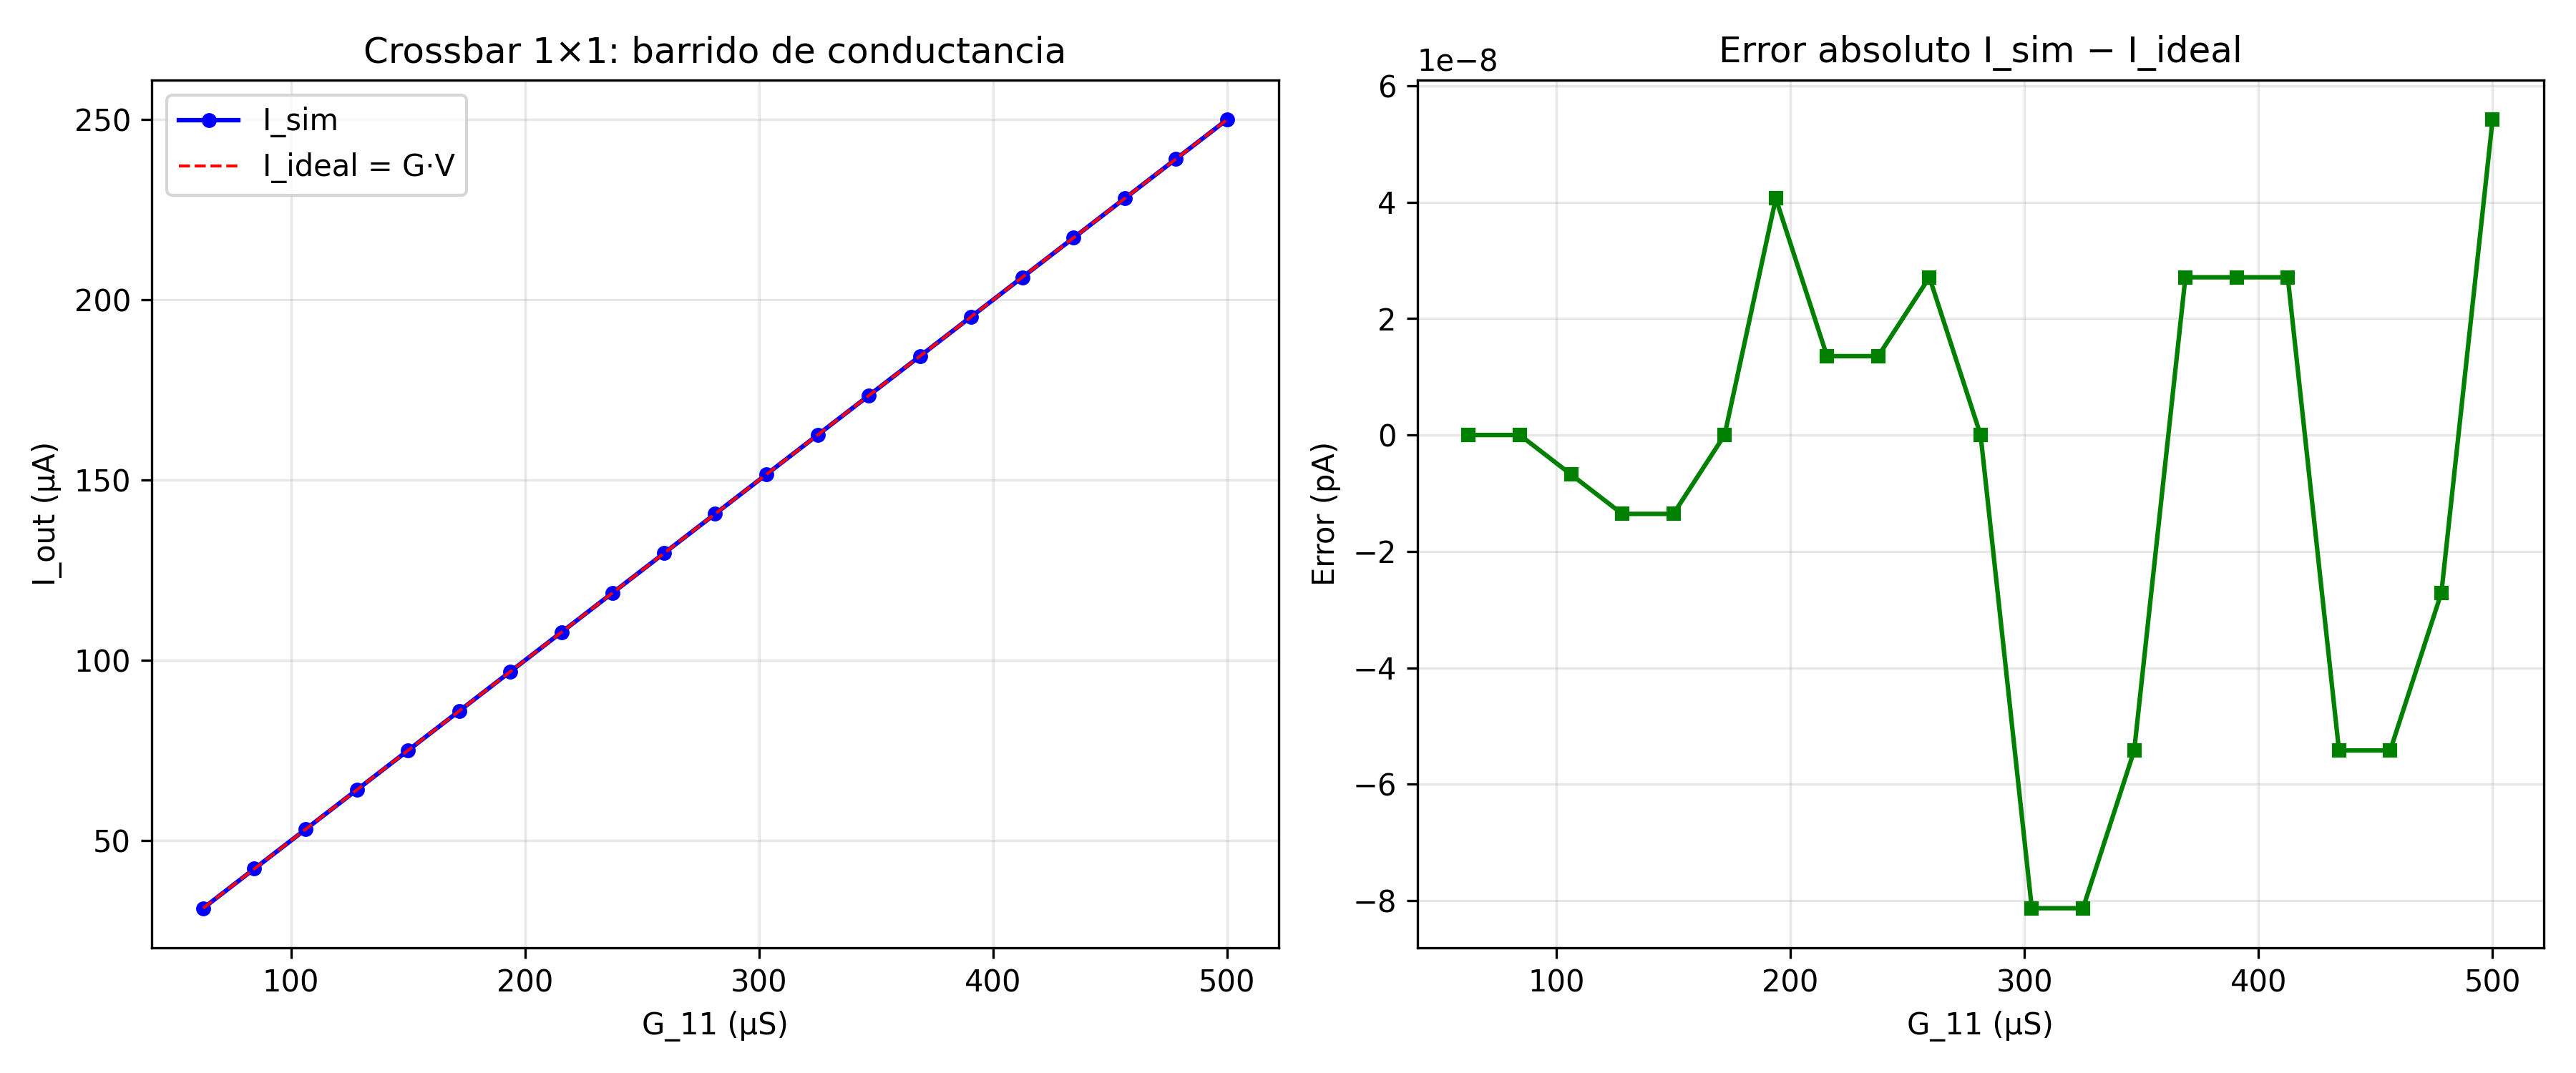
\includegraphics[width=\textwidth]{figuras/fig_21b_crossbar_G.png}
        \caption{Matriz espacial de conductancia transversal $G_{ij}(t)$.}
    \end{subfigure}
    \caption[Verificación funcional del crossbar analógico]{Verificación cualitativa y funcional de computación In-Memory en el bloque elemental Crossbar analógico (paneles a y b).}
    \label{fig:crossbar_1x1_completo}
\end{figure}

\clearpage

\begin{figure}[H]
    \ContinuedFloat
    \centering
    \begin{subfigure}[b]{0.84\textwidth}
        \centering
        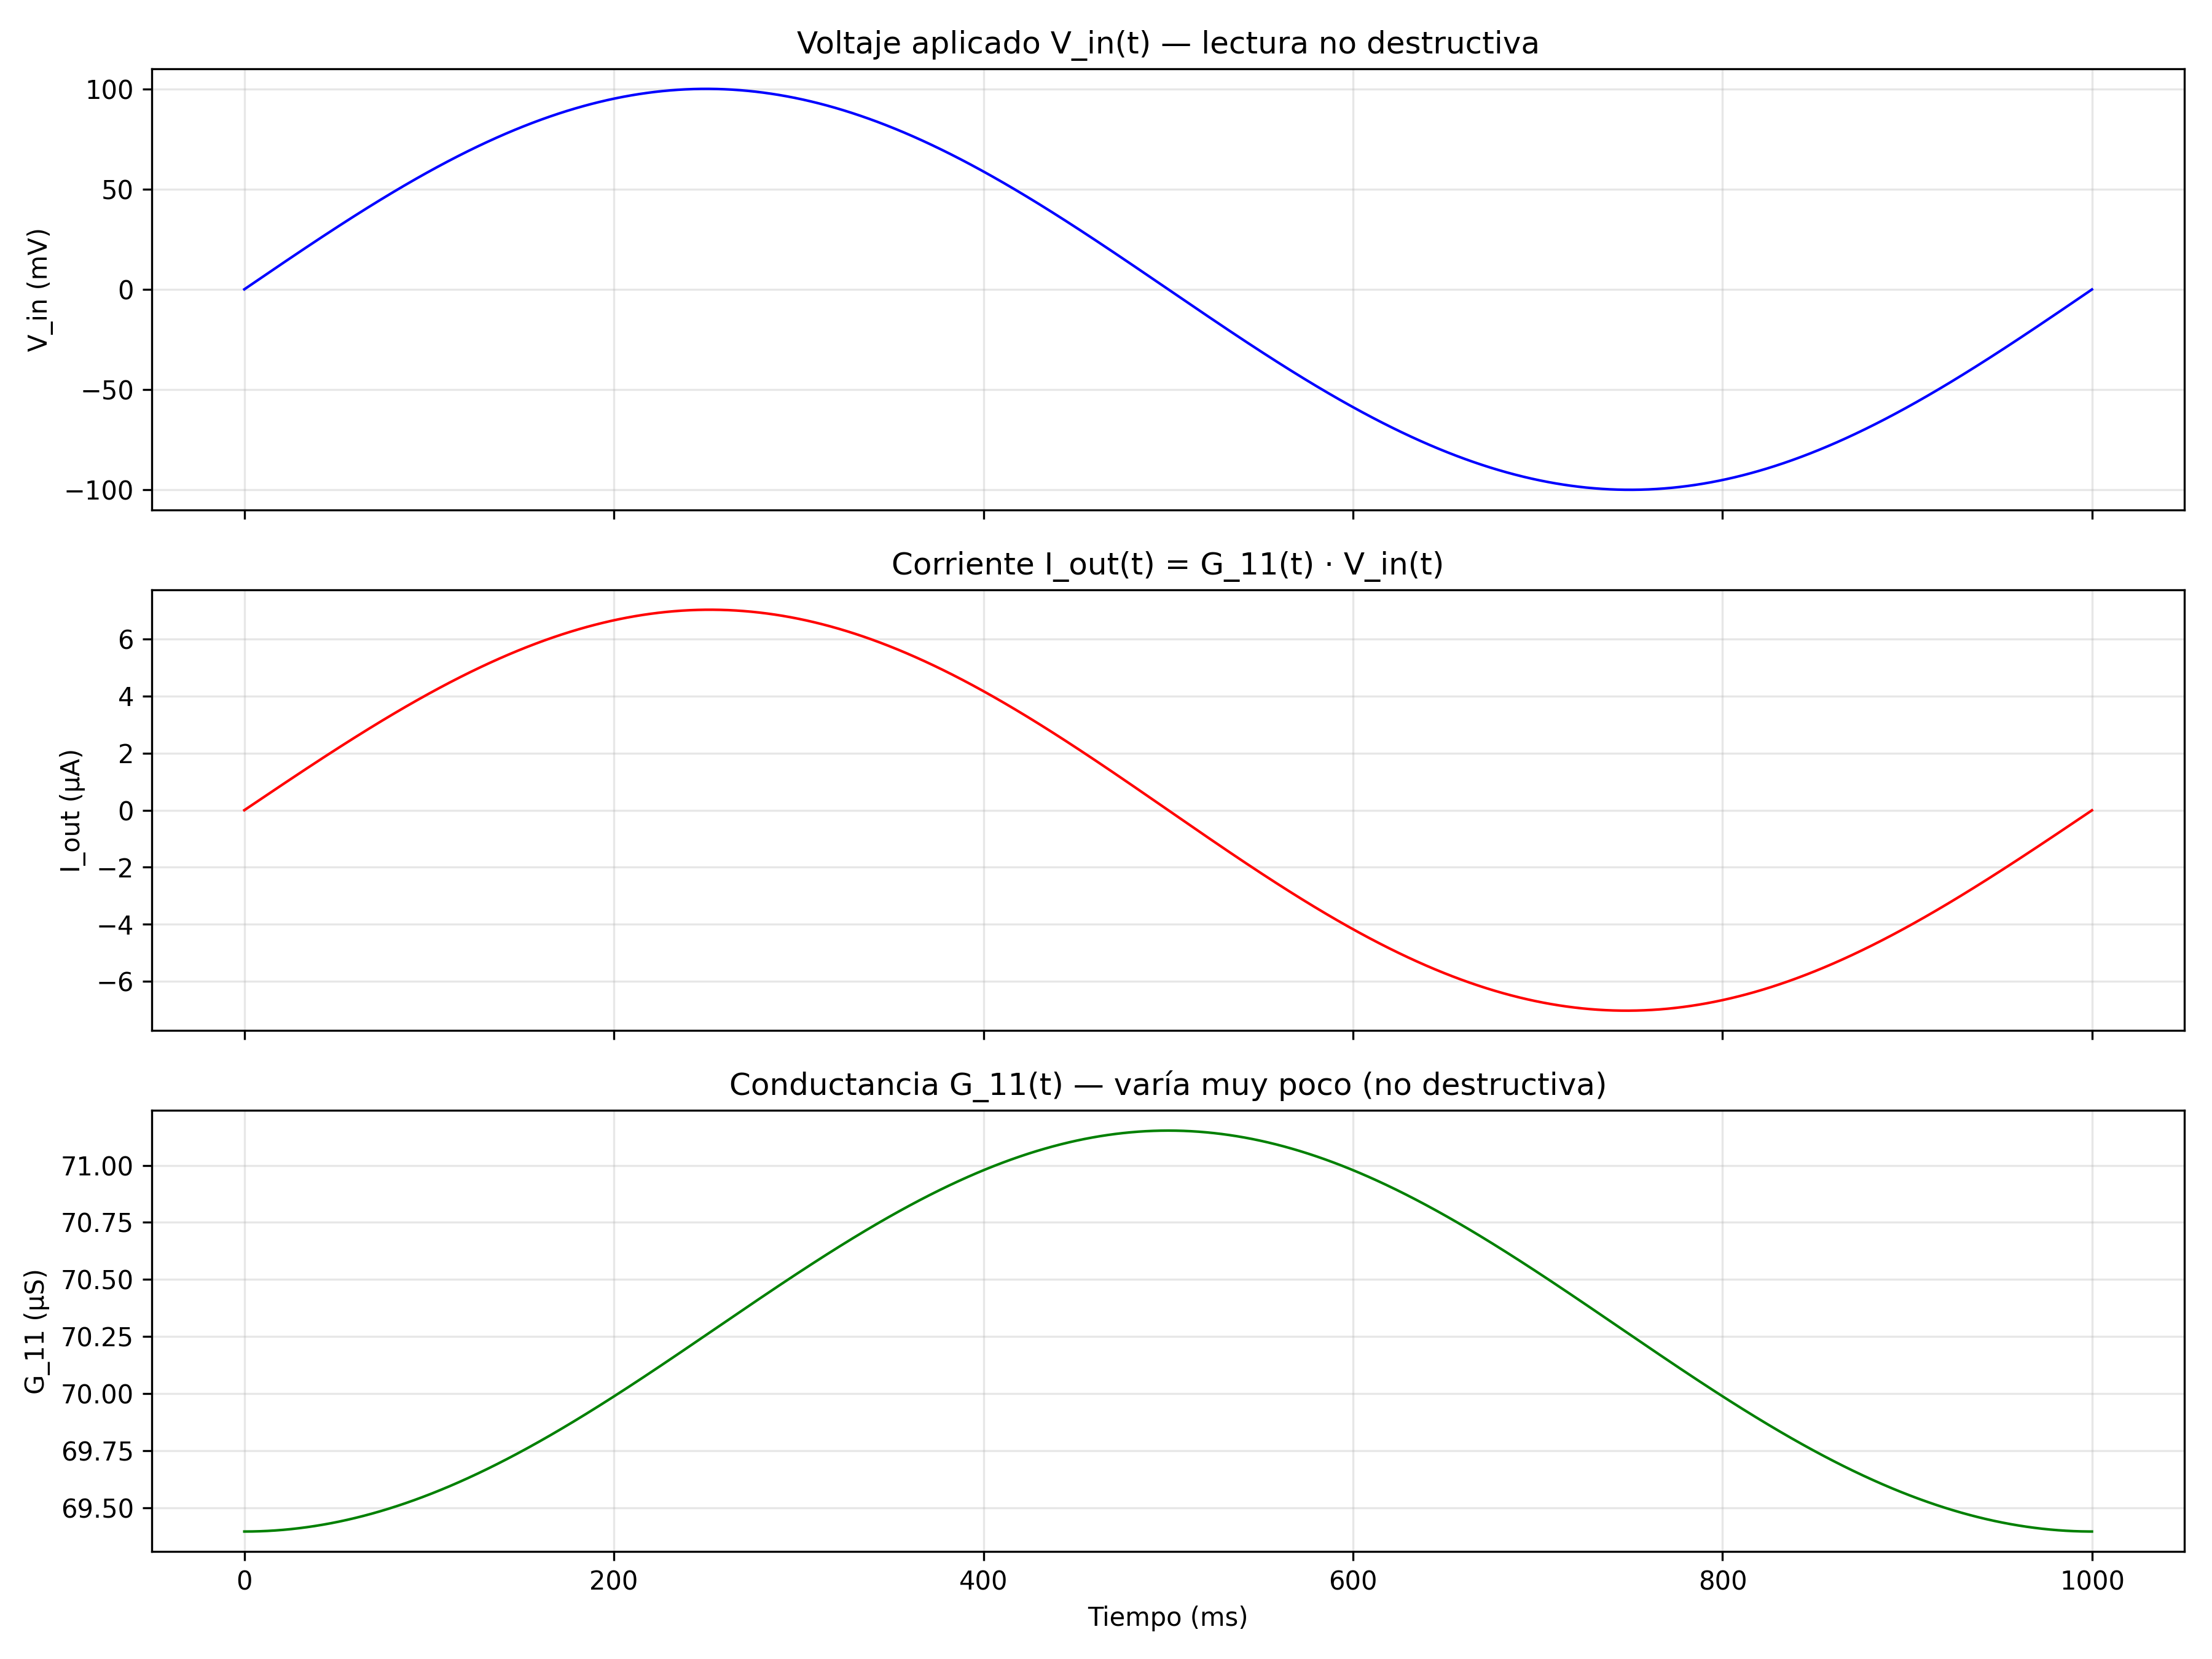
\includegraphics[width=\textwidth]{figuras/fig_21c_crossbar_din.png}
        \caption{Corrientes inferenciales recolectadas $I_j(t)$.}
    \end{subfigure}
    \vskip 0.3cm
    \begin{subfigure}[b]{0.84\textwidth}
        \centering
        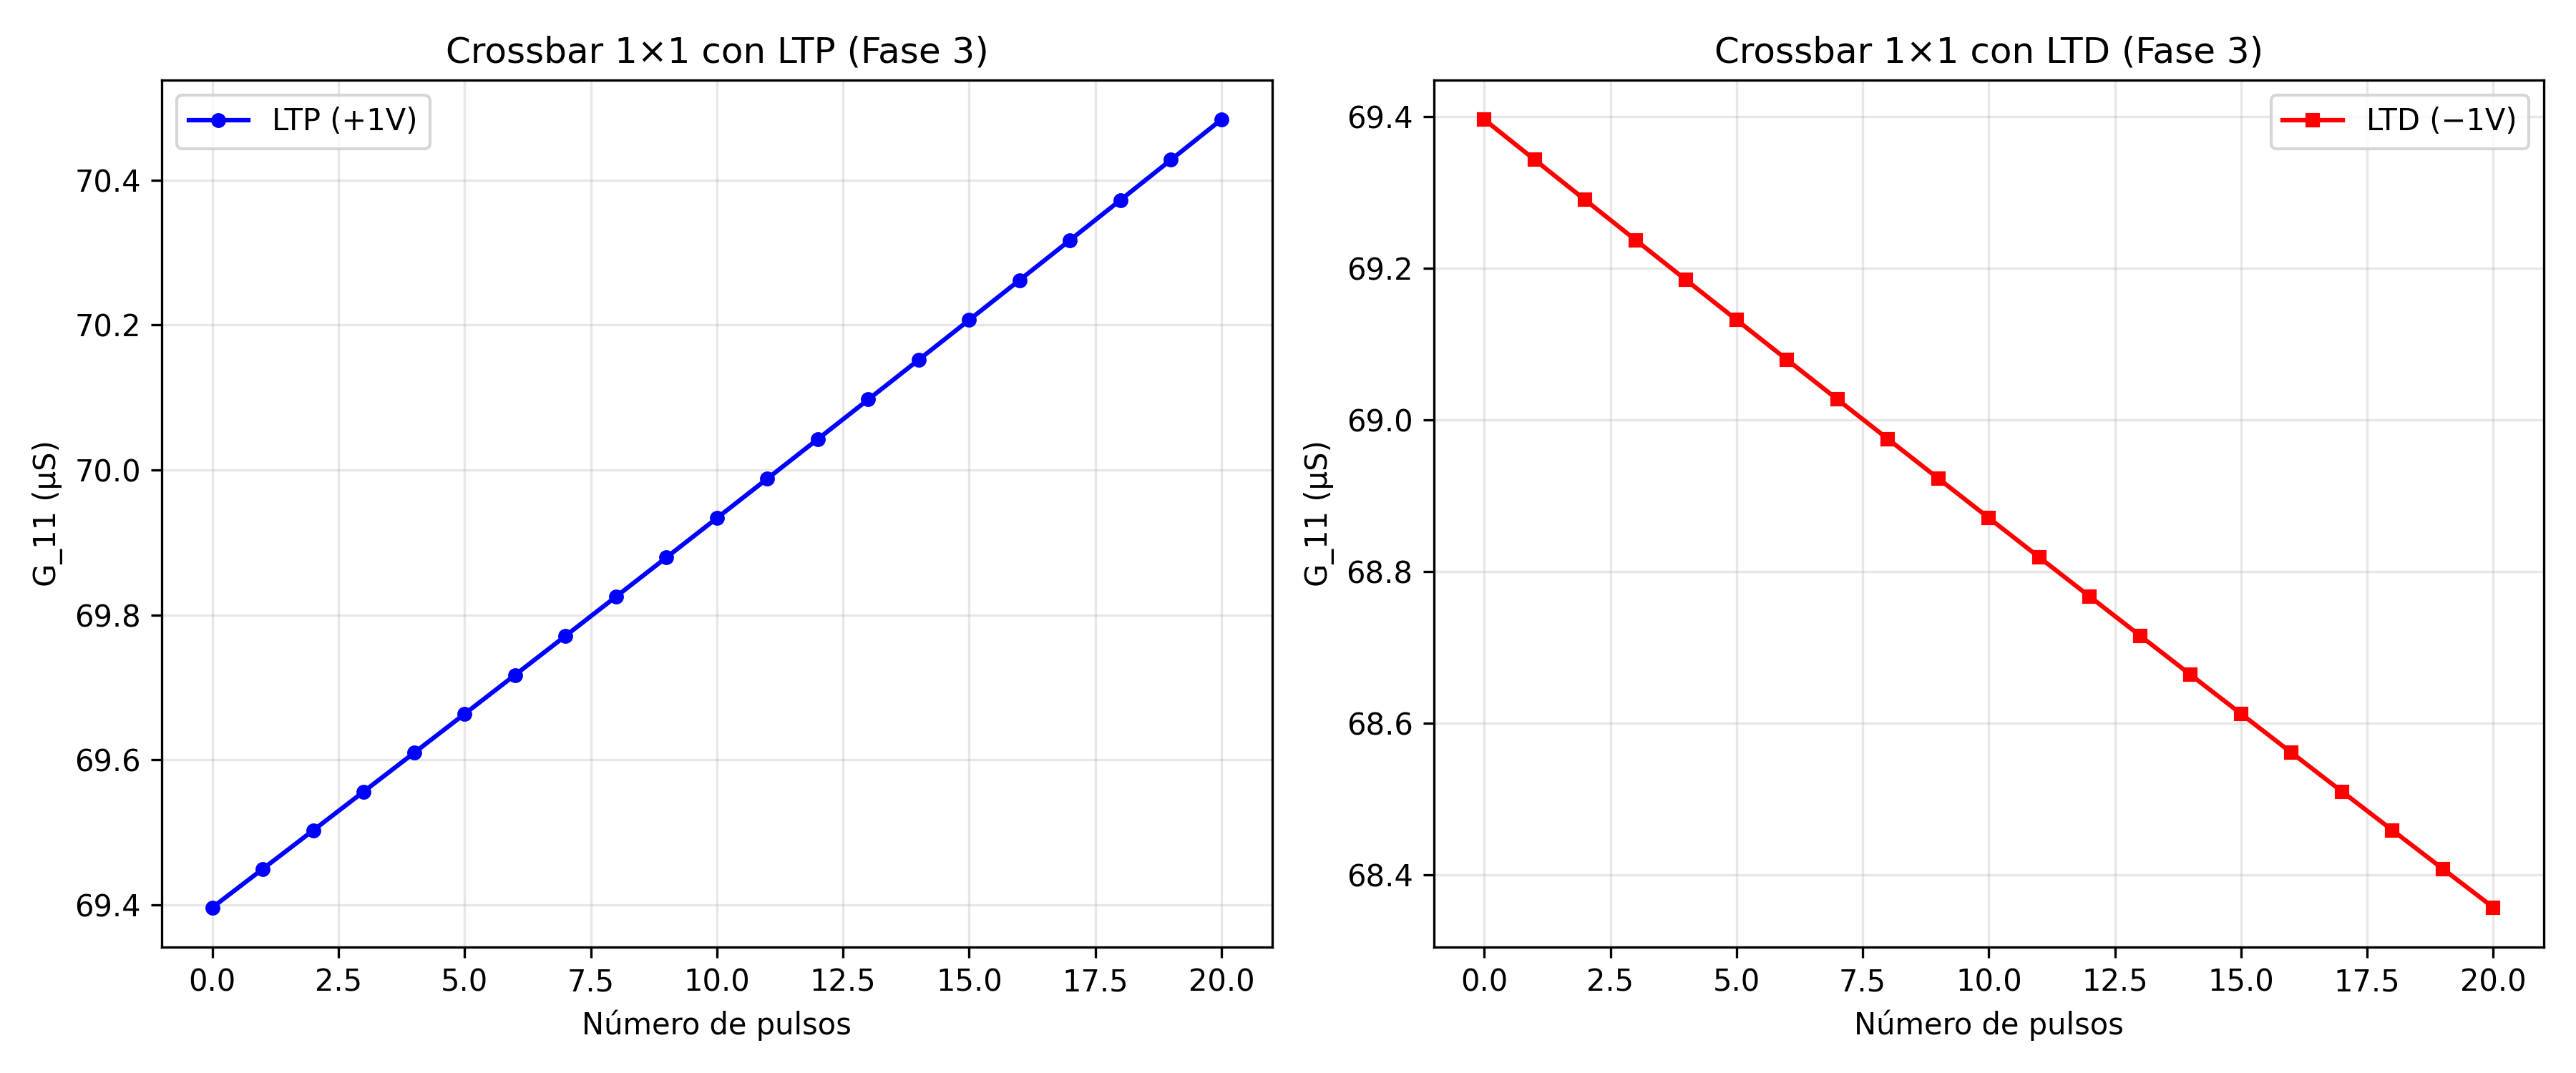
\includegraphics[width=\textwidth]{figuras/fig_21d_crossbar_stdp.png}
        \caption{Cinemática del oscilador memristivo de intersección.}
    \end{subfigure}
    \caption[]{(Continuación; paneles c y d).}
\end{figure}

\textbf{Propósito y Relevancia:} Los cuatro paneles ilustran señales y estados calculados por el modelo de simulación. No demuestran una implementación de hardware ni una ventaja temporal sobre un sistema digital.

\paragraph{Comparación cualitativa con Prezioso et al. (2015)}
La Figura~\ref{fig:prezioso_s3a} compara cualitativamente la forma de las curvas I--V generadas por el modelo local con las curvas representativas de dispositivos del panel S3a de Prezioso et al. (2015)~\cite{31}, correspondiente a la caracterización pre-forming de una porción de un crossbar $10 \times 8$. La comparación es de comportamiento y forma: el generador usa constantes locales y no carga ni digitaliza los puntos experimentales, por lo que no demuestra ajuste numérico ni concordancia punto por punto. Las Figuras~\ref{fig:prezioso_s3bc} muestran una matriz y un histograma sintéticos motivados por los paneles S3b--S3c; no reproducen las mediciones experimentales.

La curva de D-21 es paramétrica. D-22 usa una matriz sintética $4 \times 4$ de conductancias, generada con semilla fija a partir de una media y desviación estándar configuradas en el código. Ninguna de estas dos salidas representa mediciones de celdas reales ni valida ruido térmico o variabilidad medida.

\begin{figure}[H]
    \centering
    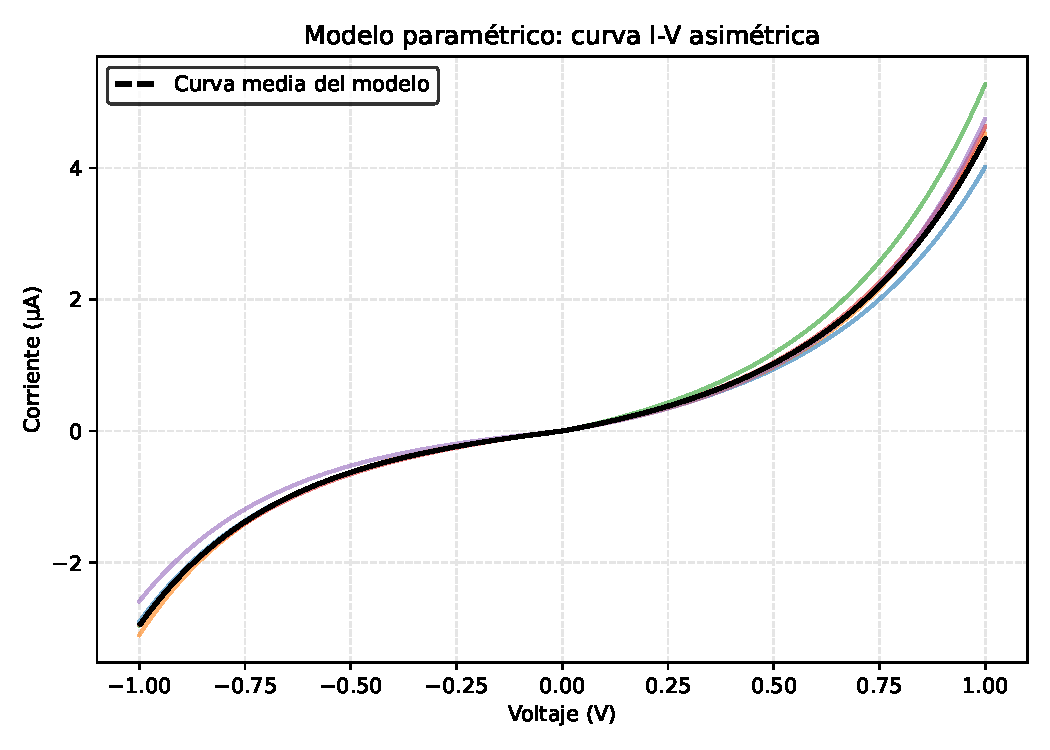
\includegraphics[width=0.85\textwidth]{figuras/23a_prezioso_s3a_modelo_ejemplo.pdf}
    \caption[Comparación cualitativa I-V con Prezioso S3a]{Comparación cualitativa de la forma I--V pre-forming con el panel S3a de Prezioso et al. (2015)~\cite{31}. Las curvas se generan con un modelo paramétrico local; no se cargan puntos digitalizados ni se afirma un ajuste cuantitativo.}
    \label{fig:prezioso_s3a}
\end{figure}

\textbf{Propósito y Relevancia:} Permite comparar visualmente el comportamiento asimétrico no lineal generado localmente con la forma de las curvas representativas del panel S3a. No acredita fidelidad de fabricación, ajuste numérico ni corrientes de fuga medidas.

\begin{figure}[H]
    \centering
    \begin{subfigure}[b]{0.48\textwidth}
        \centering
        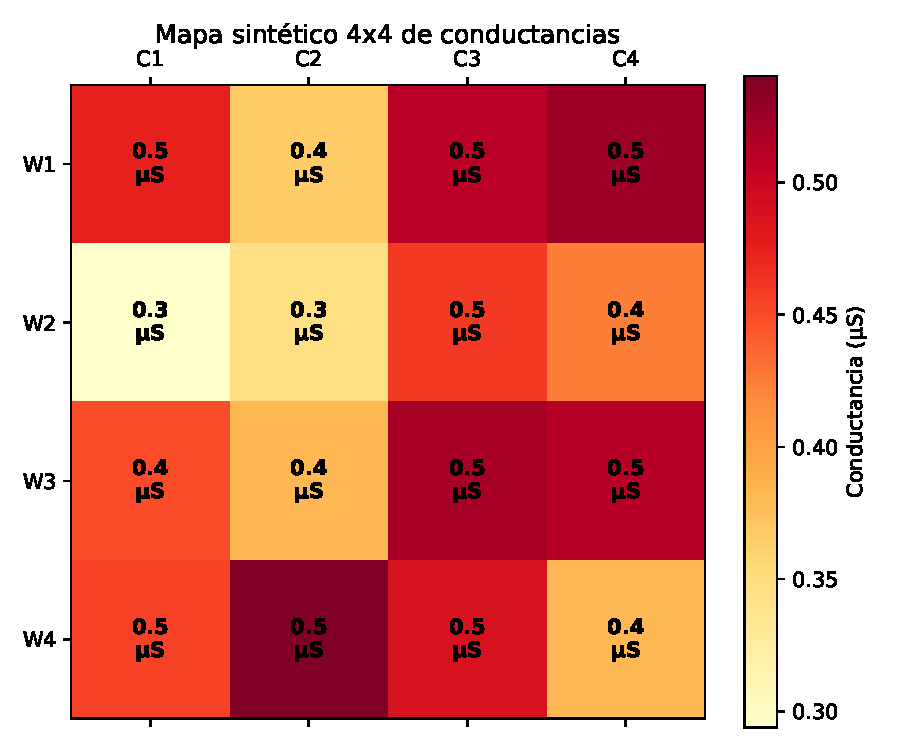
\includegraphics[width=\textwidth]{figuras/23b_prezioso_s3b_modelo_ejemplo.pdf}
        \caption{Matriz sintética de conductancias $4 \times 4$.}
    \end{subfigure}
    \hfill
    \begin{subfigure}[b]{0.48\textwidth}
        \centering
        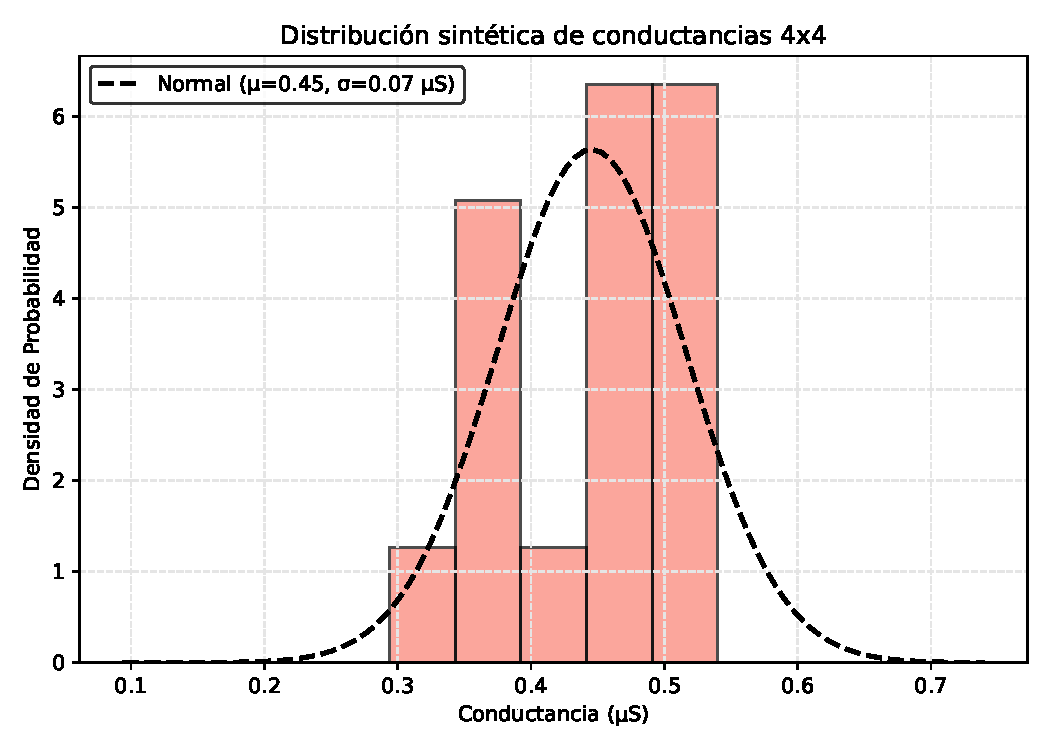
\includegraphics[width=\textwidth]{figuras/23c_prezioso_s3c_modelo_ejemplo.pdf}
        \caption{Histograma de la matriz sintética.}
    \end{subfigure}
    \caption[Ejemplos sintéticos de conductancia]{Ejemplos sintéticos de conductancias en una matriz $4 \times 4$ y su distribución. Los valores se generan en el simulador con semilla fija; no son mediciones ni una reproducción de las Figuras S3b--S3c de Prezioso et al. (2015)~\cite{31}.}
    \label{fig:prezioso_s3bc}
\end{figure}

\textbf{Propósito y Relevancia:} Ilustran la generación de una matriz virtual y un resumen estadístico de sus conductancias. No demuestran que la dispersión del simulador coincida con la variabilidad Device-to-Device del hardware reportado.

\begin{figure}[H]
    \centering
    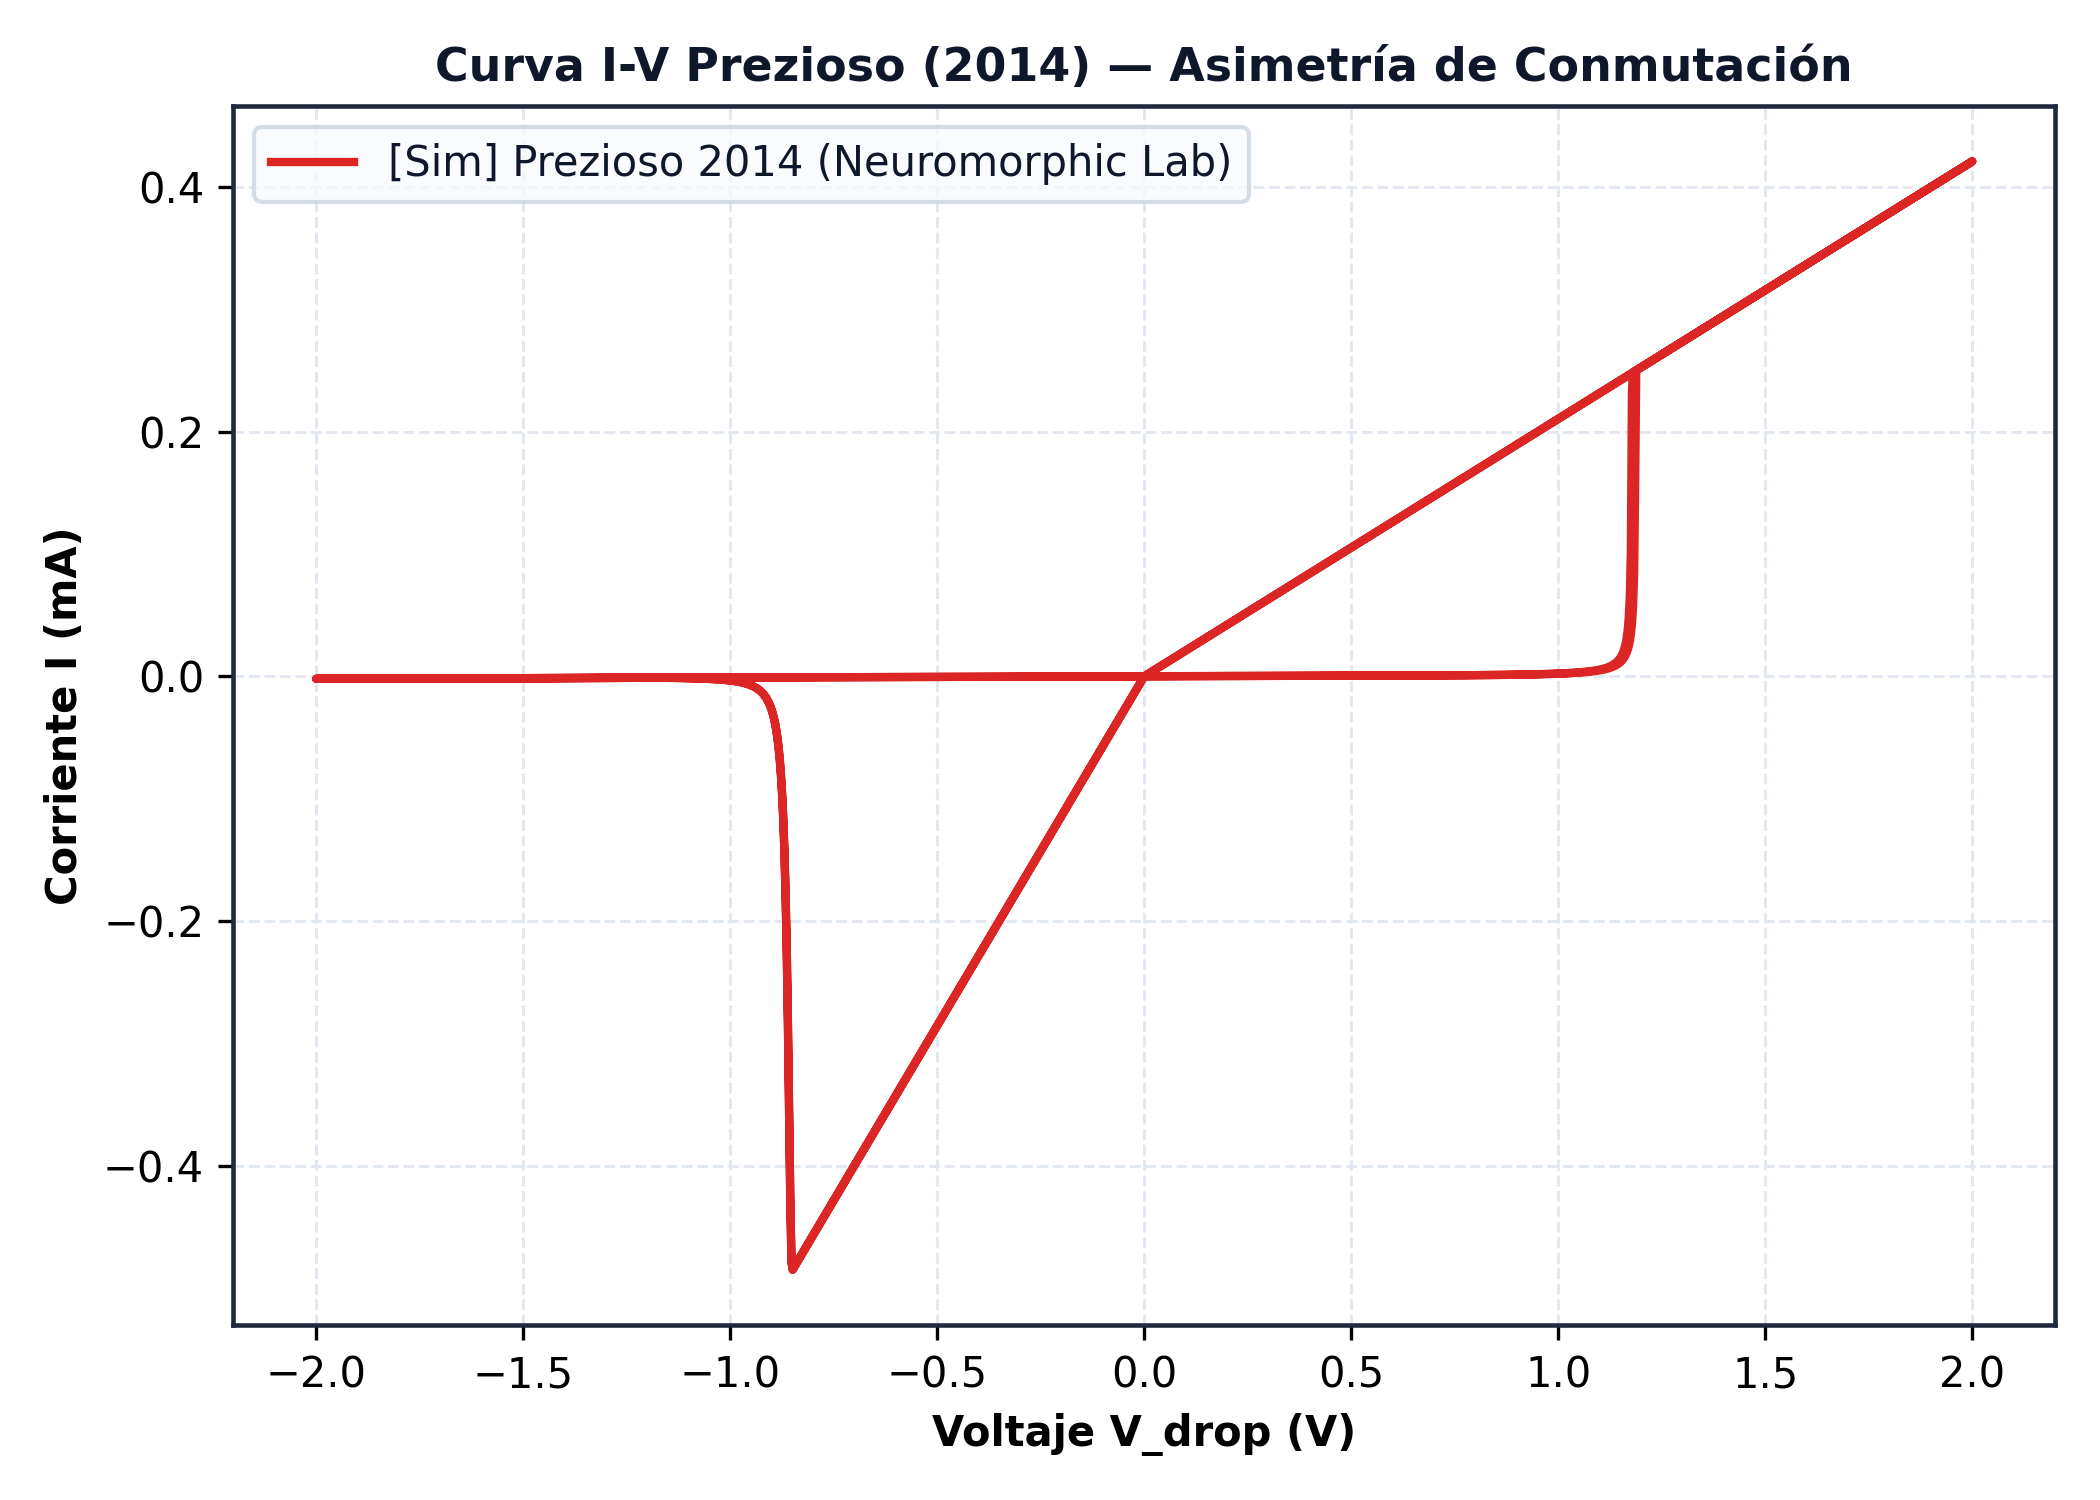
\includegraphics[width=0.7\textwidth]{figuras/fig_22_prezioso_v2.png}
    \caption{Respuesta I--V simulada con el modelo local inspirado en Prezioso et al. (2014)~\cite{3}. La curva se genera con parámetros configurados en el código; no incluye puntos experimentales ni constituye una validación cuantitativa del artículo.}
    \label{fig:22_prezioso_v2}
\end{figure}

\textbf{Propósito y Relevancia:} La figura muestra la respuesta I--V de una simulación local de un dispositivo bajo un barrido de voltaje. No muestra una matriz Crossbar ni prueba integración de sistema, escalamiento, operación SET/RESET en hardware o correspondencia cuantitativa con mediciones del artículo.


% =====================================================================
\subsubsection{Aplicación del crossbar al agente NeuroBot $24 \times 12$}
\label{sec:etapa4_2}

En esta sección se describe una arquitectura de aprendizaje por refuerzo (\textit{Reinforcement Learning}, RL) simulada: una red virtual de $24 \times 12$ acoplada al entorno CartPole. Los resultados son de simulación y no representan una validación experimental en hardware robótico o memristivo.

\paragraph{Arquitectura del Sistema ($24 \times 12$)}
El cerebro neuromórfico del agente consiste en un crossbar memristivo de $N=24$ filas de entrada y $M=12$ columnas de salida.

\subparagraph{Codificador de Estados (Encoder Top-K)}
El vector de observación continuo $\mathbf{s} = [x, \dot{x}, \theta, \dot{\theta}] \in \mathbb{R}^4$ se proyecta mediante una batería de receptores gaussianos distribuidos a lo largo del dominio de cada variable. Se aplica un mecanismo Top-K ($K=10$) que selecciona las 10 filas de mayor activación, generando un patrón binario disperso de voltajes de lectura $V_{\text{rows}} \in \{0, V_{\text{read}}\}$.

\subparagraph{Crossbar Memristivo y Solución Nodal (MNA)}
La corriente integrada por columna $\mathbf{I}_{\text{col}} \in \mathbb{R}^{12}$ se calcula resolviendo la matriz MNA con resistencia de línea $R_{\text{wire}} = 10^{-3}\,\Omega$ y resistencia de sensado $R_{\text{sense}} = 100\,\Omega$:
\begin{equation}
    \mathbf{I}_{\text{col}} = \text{MNA}(\mathbf{G}, V_{\text{rows}}, R_{\text{wire}}, R_{\text{sense}})
\end{equation}
donde $G_{ij} = \frac{1}{R_{\text{on}} + X_{ij}(R_{\text{off}} - R_{\text{on}})}$ representa la conductancia de la celda en el estado interno $X_{ij} \in [0, 1]$.

\subparagraph{Decodificador y Acción (Softmax e Inercia de Motor)}
Las 12 columnas se agrupan en pares de conductancias asociadas a 6 niveles discretos de fuerza activa para giro hacia la izquierda ($1 - 30\,\text{N}$) y 6 para la derecha ($1 - 30\,\text{N}$). La probabilidad de selección de acción $\pi_j$ sigue una distribución Softmax parametrizada por la temperatura ambiental $T$:
\begin{equation}
    \pi_j = \frac{\exp(I_j / T)}{\sum_{k=1}^M \exp(I_k / T)}
\end{equation}
Se aplica una tasa de cambio (slew rate) de $50/50$ en la dinámica del actuador para simular la inercia del motor robótico real.

\paragraph{REINFORCE con baseline}
El aprendizaje del agente no es STDP: es REINFORCE con baseline y ocurre al final de cada episodio:
\begin{equation}
    \Delta X_{ij} = -\eta \cdot E_{ij} \cdot (R_{\text{ep}} - b)
\end{equation}
donde $E_{ij}$ es la elegibilidad acumulada por paso a partir de $\mathrm{pre}_i(t)(\mathbf{1}_{j=a(t)}-\pi_j(t))$, con decaimiento $\gamma$ entre pasos. No se usa una ventana de STDP entre disparos pre y postsinápticos ni una traza de memristores volátiles; $E$ se mantiene como acumulador matemático del agente.

Con la convención $X=1-x$, una ventaja positiva produce
$\Delta X<0$ en la columna elegida cuando su elegibilidad es positiva;
esto reduce su resistencia y aumenta su conductancia. La prueba
unitaria del agente comprueba este signo en un caso controlado, sin
demostrar convergencia general ni equivalencia con STDP.

La actualización $\Delta X$ utiliza recorte por norma de gradiente
($\max|\Delta X| \le 0.05$) y se congela si
$R_{\text{ep}} \ge 430$. Este umbral es un criterio operativo del
protocolo evaluado y no demuestra que la política alcanzada sea óptima.

\paragraph{Resultados de simulación y discusión en control robótico}

Los valores de recompensa y ablación de esta sección proceden de
registros de simulación previamente reportados. No se reejecutaron las
cinco semillas ni las ablaciones durante esta revisión; por tanto, se
presentan como resultados reportados, no como cifras reproducidas aquí
ni como resultados experimentales de hardware.

\subparagraph{Convergencia y Reproducibilidad Multi-Semilla}
Se ejecutaron cinco semillas (0--4), con 300 episodios cada una, $V_{\mathrm{read}}=0.05$ V, D2D ($\sigma=0.08$), C2C ($\sigma=0.05$, $\theta=1\,\mathrm{s}^{-1}$, $dt=0.02\,\mathrm{s}$) y congelamiento de la actualización de pesos para $R_{\mathrm{ep}}\geq430$. Las recompensas medias de los últimos 200 episodios fueron 369.66, 421.44, 474.31, 462.79 y 448.36, respectivamente; la media entre semillas fue 435.31 y su desviación estándar 37.28. Cuatro corridas alcanzaron al menos una recompensa episódica de 480; la semilla 3 tuvo máximo 479.14. Los registros se guardan como \texttt{run\_24x12\_A\_d2d\_c2c\_seed0.json}--\texttt{seed4.json}; la figura y discusión se presentan en la Sección~3.4.1.

La media de la semilla 0 debe interpretarse considerando su trayectoria:
las recompensas medias por bloques de 50 episodios fueron 13.90,
58.55, 99.39, 470.69, 461.27 y 447.29. Su primera media móvil de
20 episodios que alcanzó 430 apareció en el episodio 157. Así, el
promedio de los episodios 101--300 (369.66) refleja en buena medida el
tiempo que tardó esta corrida en alcanzar recompensas altas y no basta
para concluir que la semilla sea intrínsecamente peor. Este cruce es
un indicador operativo de adquisición de desempeño, no una
demostración formal de convergencia; el análisis detallado se presenta
en la Sección~\ref{sec:res_cartpole}.

\subparagraph{Estudio de Ablaciones}
Para validar la contribución de cada bloque del agente, se evaluaron cuatro configuraciones (Figura~\ref{fig:ablaciones_robot}):
\begin{itemize}
    \item \textbf{A (Control Base):} Sistema completo con decaimiento térmico y traza acumulativa ($\bar{R} \approx 491.9$ en semillas exitosas, $60\%$ de tasa de convergencia en 5 semillas aleatorias).
    \item \textbf{B (Sin Adaptación Térmica, $T=0.10$ Fijo):} Colapso por congelamiento estocástico ($\bar{R} = -39.0$). Demuestra que sin alta exploración inicial, el agente congela la búsqueda de políticas.
    \item \textbf{C (Sin Traza de Elegibilidad, $\varepsilon=0$):} Colapso total ($\bar{R} = -33.3$, $\Delta X=0$), evidenciando que la elegibilidad acumulada es necesaria en la configuración REINFORCE evaluada.
    \item \textbf{D (Hebbiano Sin Modulación $R_{\text{ep}}-b$):} Divergencia y colapso ($\bar{R} = -39.0$) por falta del escalar de refuerzo global.
\end{itemize}

\begin{figure}[H]
    \centering
    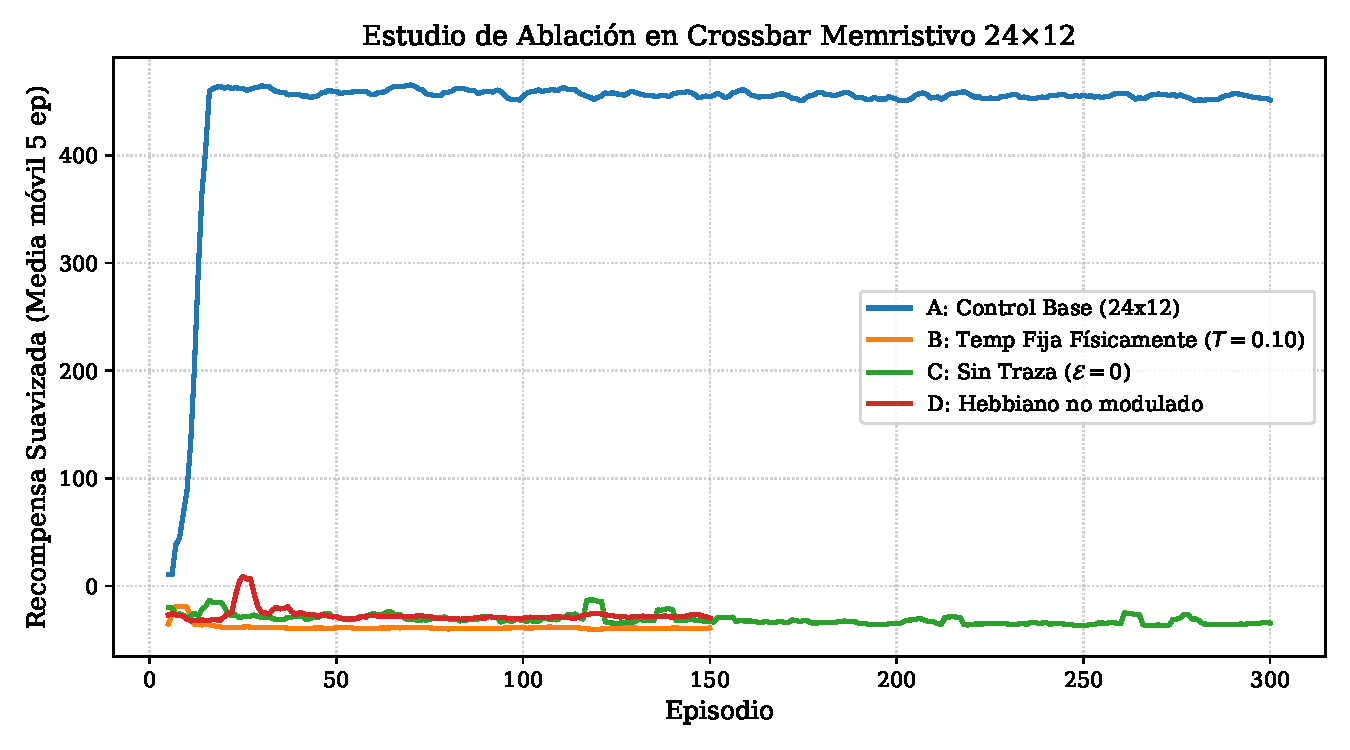
\includegraphics[width=0.85\textwidth]{figuras/comparativa_ablaciones_24x12.pdf}
    \caption{Estudio de ablación comparativo (A, B, C, D) en el crossbar $24 \times 12$.}
    \label{fig:ablaciones_robot}
\end{figure}

\subparagraph{Heatmap de la Matriz Memristiva Consolidada ($X$)}
La Figura~\ref{fig:heatmap_robot} muestra la distribución final del estado memristivo $X \in [0, 1]$. Se observa una estructura bimodal no saturada ($\mu = 0.165, \sigma = 0.118$) con bandas claras de activación sináptica diferenciadas por la velocidad y el ángulo del poste.

\begin{figure}[H]
    \centering
    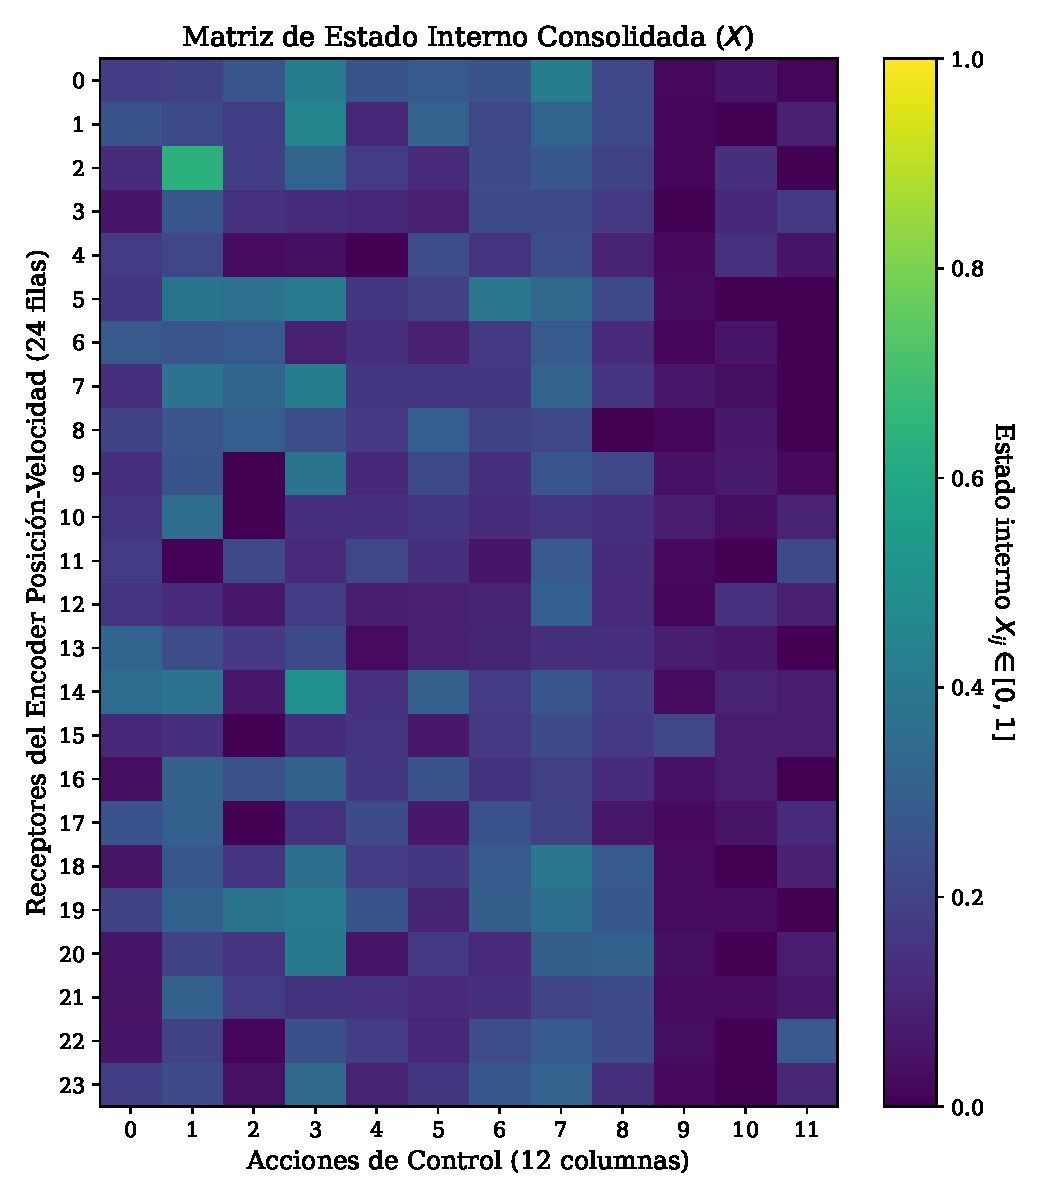
\includegraphics[width=0.65\textwidth]{figuras/heatmap_matriz_X_24x12.pdf}
    \caption{Heatmap de la variable de estado interno $X$ tras el entrenamiento del agente; la conductancia $G$ se deriva de $X$ y no se muestra en esta figura.}
    \label{fig:heatmap_robot}
\end{figure}


% =====================================================================
\subsubsection{Validación del Modelo Físico del Crossbar (Suite de 10 Experimentos)}
\label{sec:suite_10_exp}

La suite consta de 10 experimentos de simulación autónomos del modelo
crossbar. Las cifras que siguen son las consignadas en sus informes y
figuras existentes; no se reejecutaron ni se verificaron de nuevo sus
registros de entrada en esta revisión. Por ello describen resultados
reportados del modelo, no una certificación de fidelidad respecto a
hardware real. Las condiciones de excitación y las impedancias de
sensado ($R_{\text{sense}} = 100\,\Omega$) se atribuyen a la
configuración declarada para el agente.

\paragraph{Exp.~1 --- Error de lectura del crossbar vs.\ tamaño}

La Figura~\ref{fig:exp01} cuantifica el error relativo de lectura del arreglo
al escalar de $N=4$ a $N=32$ filas con $M=12$ columnas fijas. Se define el
error relativo como
$\varepsilon = \|I_{\text{col}} - I_{\text{ideal}}\| / \|I_{\text{ideal}}\|$,
donde $I_{\text{col}}$ es la solución nodal del arreglo (MNA con
$R_{\text{wire}}$ y $R_{\text{sense}}$) e $I_{\text{ideal}} = \mathbf{G}^T \mathbf{V}$
es la proyección lineal ideal.

Para $N=4$ el error es $\varepsilon \approx 6.5\%$ y escala monótonamente
hasta $\varepsilon \approx 41\%$ para $N=32$. Este crecimiento refleja la
contribución conjunta de la caída resistiva en las líneas ($R_{\text{wire}}$)
y el divisor formado por $R_{\text{sense}}$ con la conductancia agregada del
arreglo. El efecto de corrientes parásitas estrictas (\textit{sneak paths} en
el sentido clásico: fila única activa con filas flotantes) requiere una
configuración de excitación distinta y se considera una extensión natural
para trabajos futuros.

\begin{figure}[H]
  \centering
  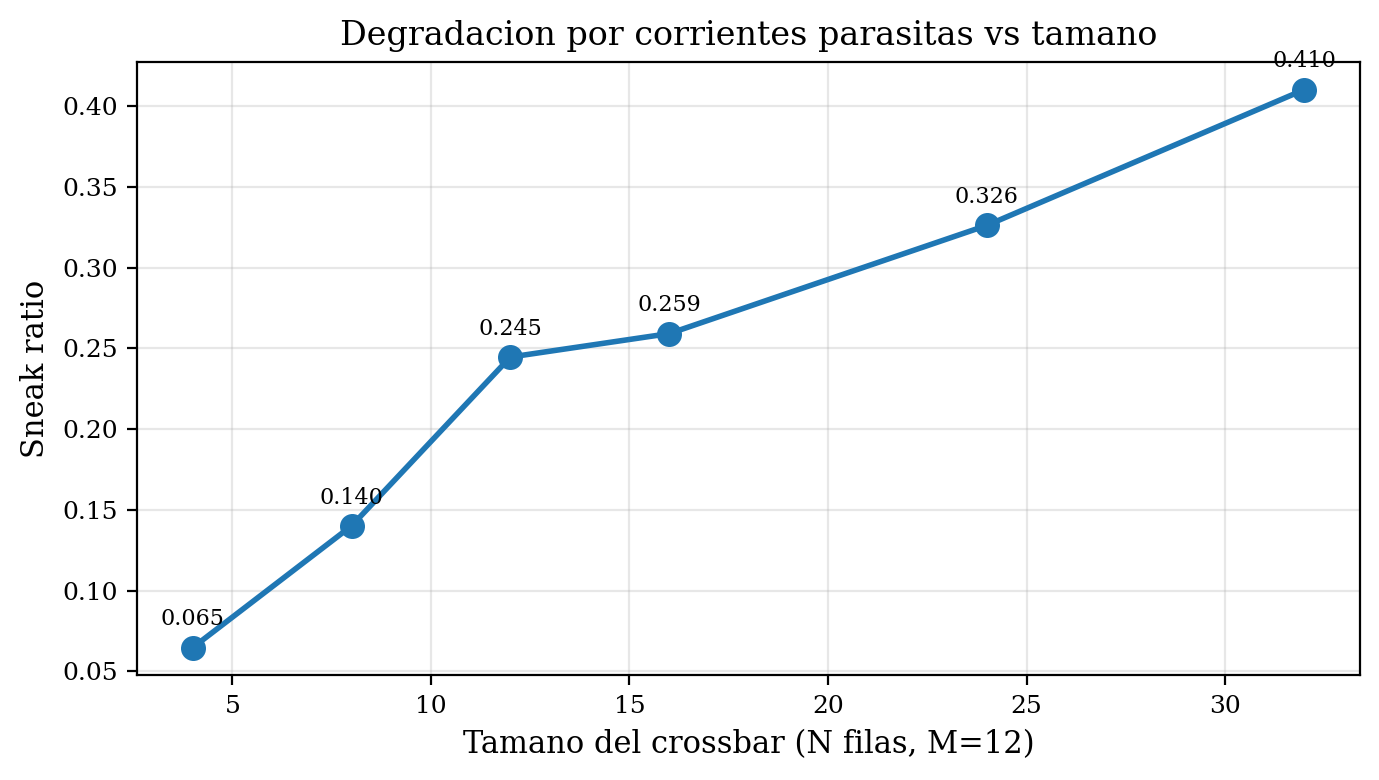
\includegraphics[width=0.65\textwidth]{experiments/figures/exp01_sneak_vs_N.png}
  \caption{Error relativo de lectura vs.\ tamaño del arreglo. Crecimiento
  monótono desde $N=4$ ($6.5\%$) hasta $N=32$ ($41\%$).}
  \label{fig:exp01}
\end{figure}

\paragraph{Exp.~2 --- MNA real vs.\ modelo ideal}
La Figura~\ref{fig:exp02} compara corrientes MNA e ideales para cuatro tamaños. En el caso $N=24$, el error medio por componente alcanza $29.08\%$, reflejando la contribución acumulada de $R_{\text{wire}}$ y $R_{\text{sense}}$ sobre las corrientes de columna.
\begin{figure}[H]
  \centering
  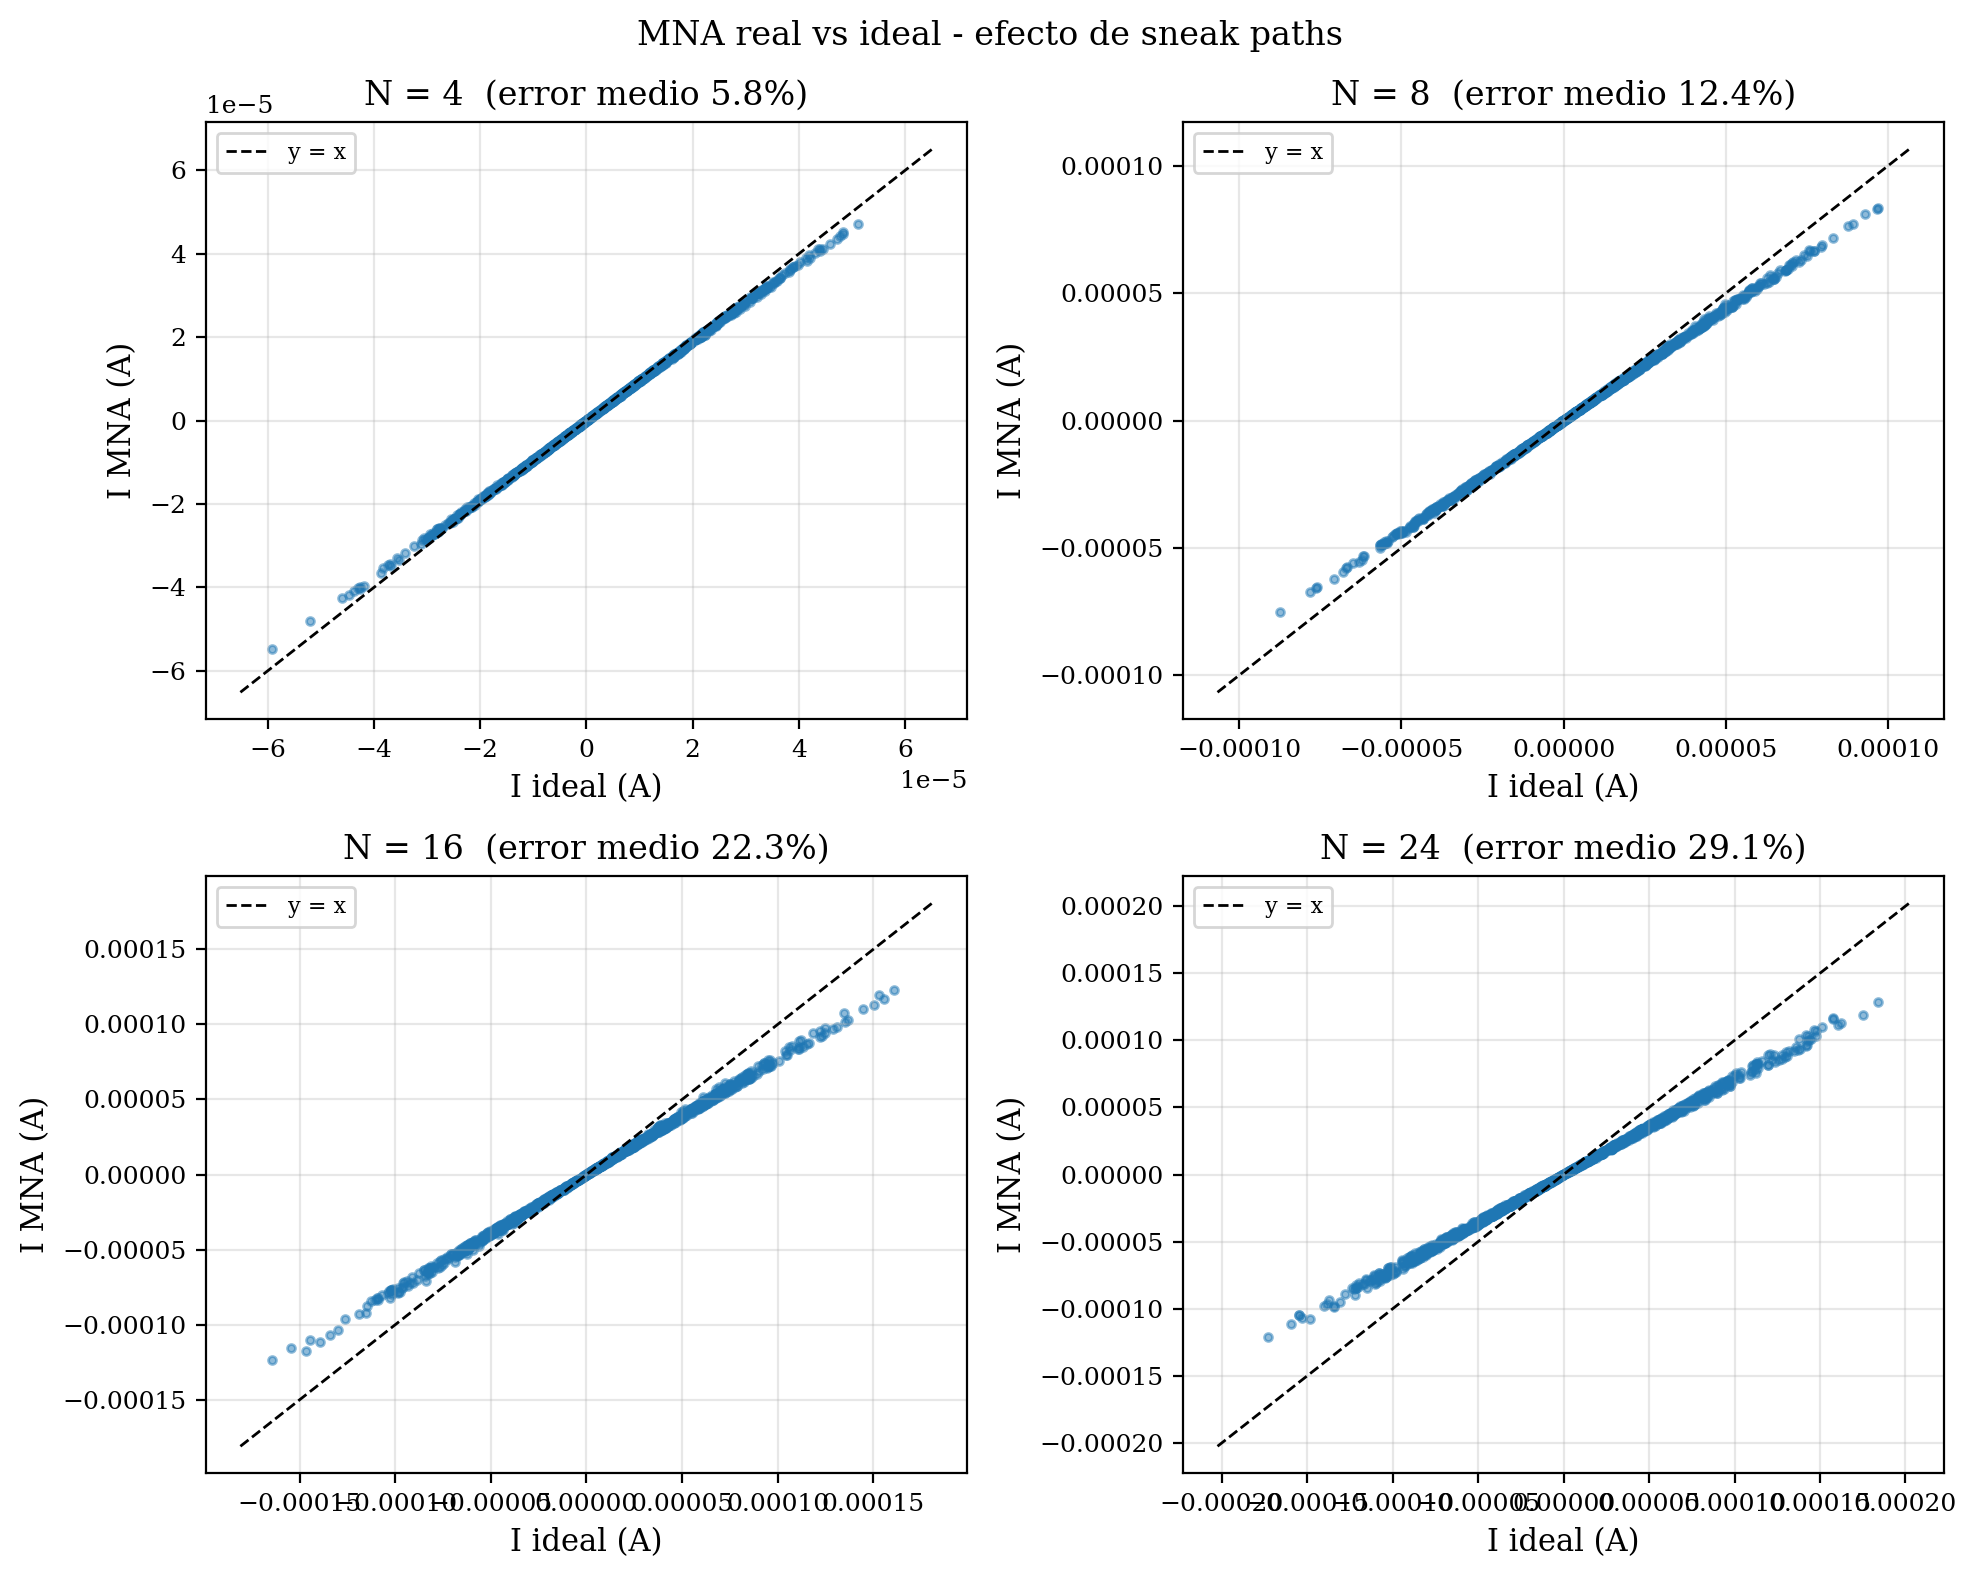
\includegraphics[width=0.90\textwidth]{experiments/figures/exp02_mna_vs_ideal.png}
  \caption{Diagrama de dispersión MNA vs.\ Ideal. El error crece de forma no lineal con $N$.}
  \label{fig:exp02}
\end{figure}

\paragraph{Exp.~3 --- Caída de tensión en línea ($R_{\text{wire}}$)}
La Figura~\ref{fig:exp03} ilustra cómo $R_{\text{wire}}$ distorsiona el perfil de corriente. El efecto sobre el perfil es doble: atenúa la corriente media ($-13\%$ entre $R_{\text{wire}} = 1\,\text{m}\Omega$ y $R_{\text{wire}} = 10\,\Omega$) y mantiene prácticamente invariante la no-uniformidad relativa entre columnas ($\sim 27\%$), dominada por la dispersión dispositivo-a-dispositivo de $\mathbf{G}$.
\begin{figure}[H]
  \centering
  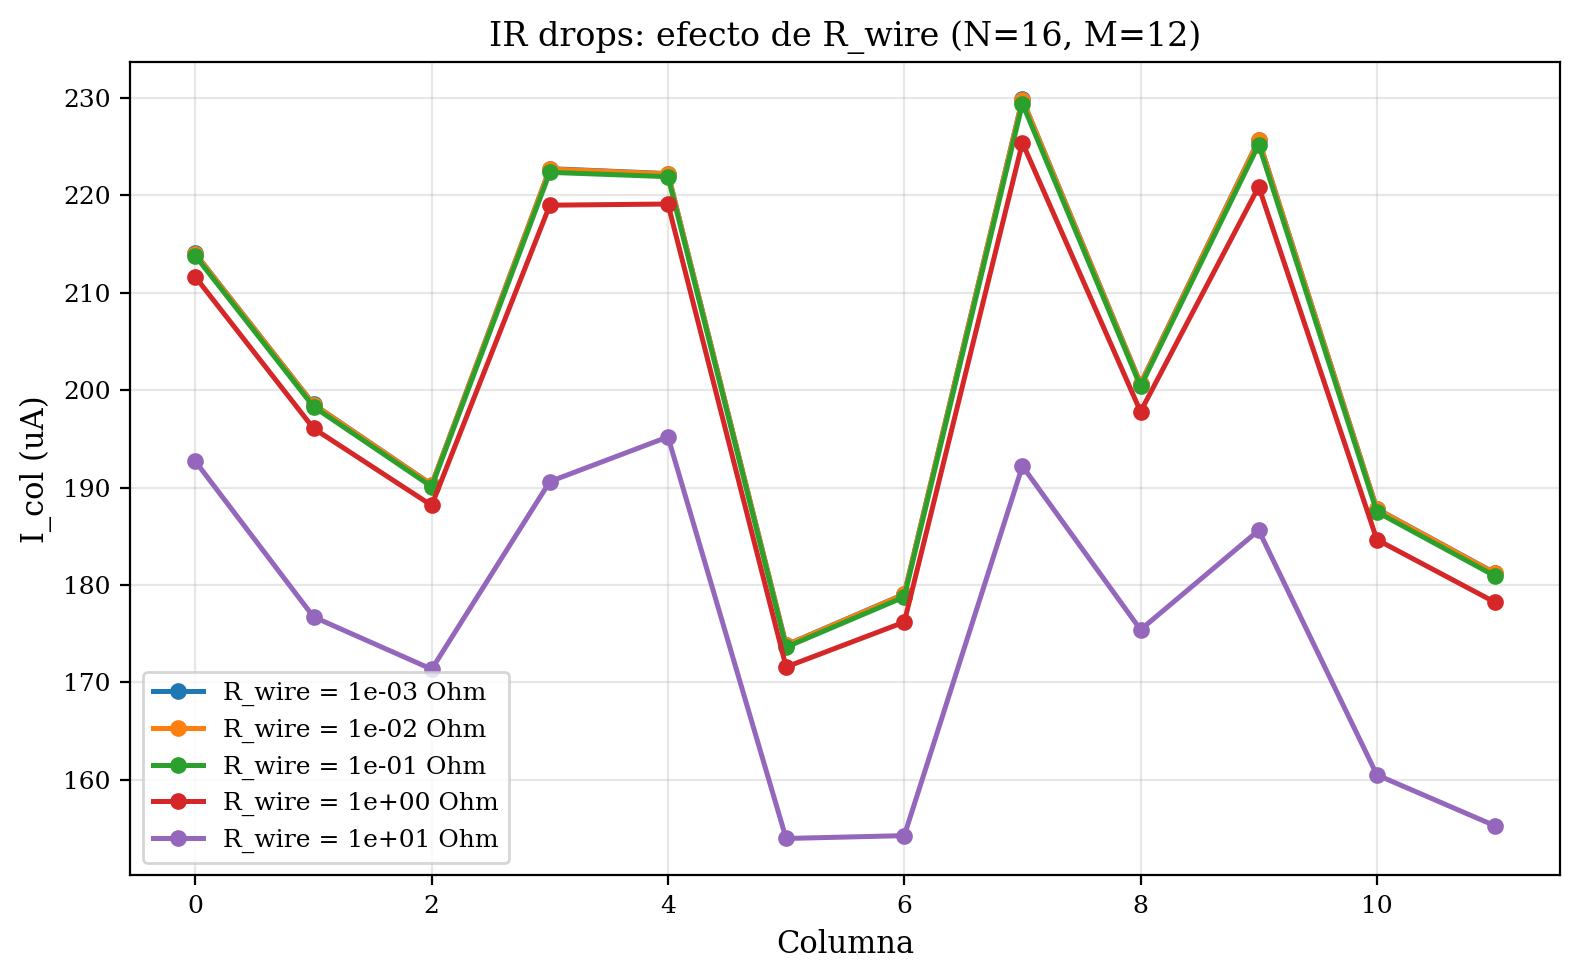
\includegraphics[width=0.72\textwidth]{experiments/figures/exp03_rwire_effect.png}
  \caption{Perfil de $I_{\text{col}}$ para distintos $R_{\text{wire}}$. La
atenuación de la corriente media aumenta con la resistencia de línea, mientras
que la dispersión entre columnas se mantiene dominada por la variabilidad de
$\mathbf{G}$.}
  \label{fig:exp03}
\end{figure}

\paragraph{Exp.~4 --- Precisión en VMM}
La Figura~\ref{fig:exp04} muestra la distribución del error relativo en VMM para 1000 vectores aleatorios. El error medio crece de $5.82\%$ ($N=4$) a $29.05\%$ ($N=24$).
\begin{figure}[H]
  \centering
  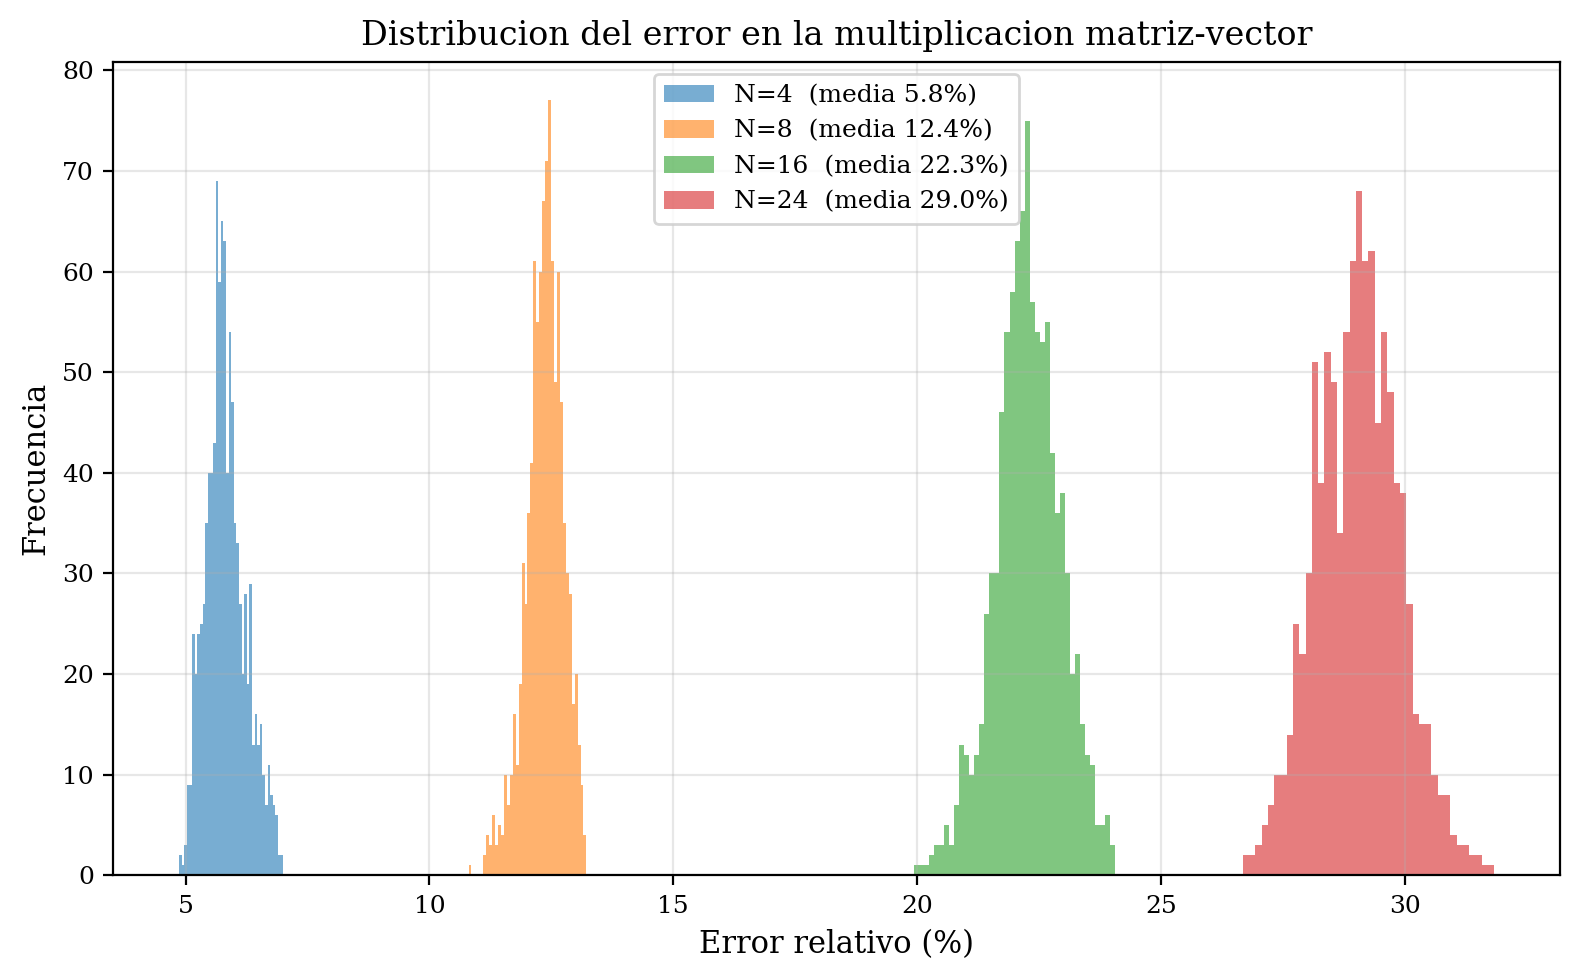
\includegraphics[width=0.70\textwidth]{experiments/figures/exp04_vmm_precision.png}
  \caption{Histograma del error relativo en VMM por tamaño de crossbar.}
  \label{fig:exp04}
\end{figure}

\paragraph{Exp.~5 --- Half-select disturb simulado: V/2 vs.\ V/3}
La Figura~\ref{fig:exp05} compara la perturbación calculada por el modelo para celdas \textit{half-selected}. Los valores reportados son 50.0\% para V/2 y 33.3\% para V/3; son razones de excitación del protocolo simulado, no medidas de disturb en celdas fabricadas.
\begin{figure}[H]
  \centering
  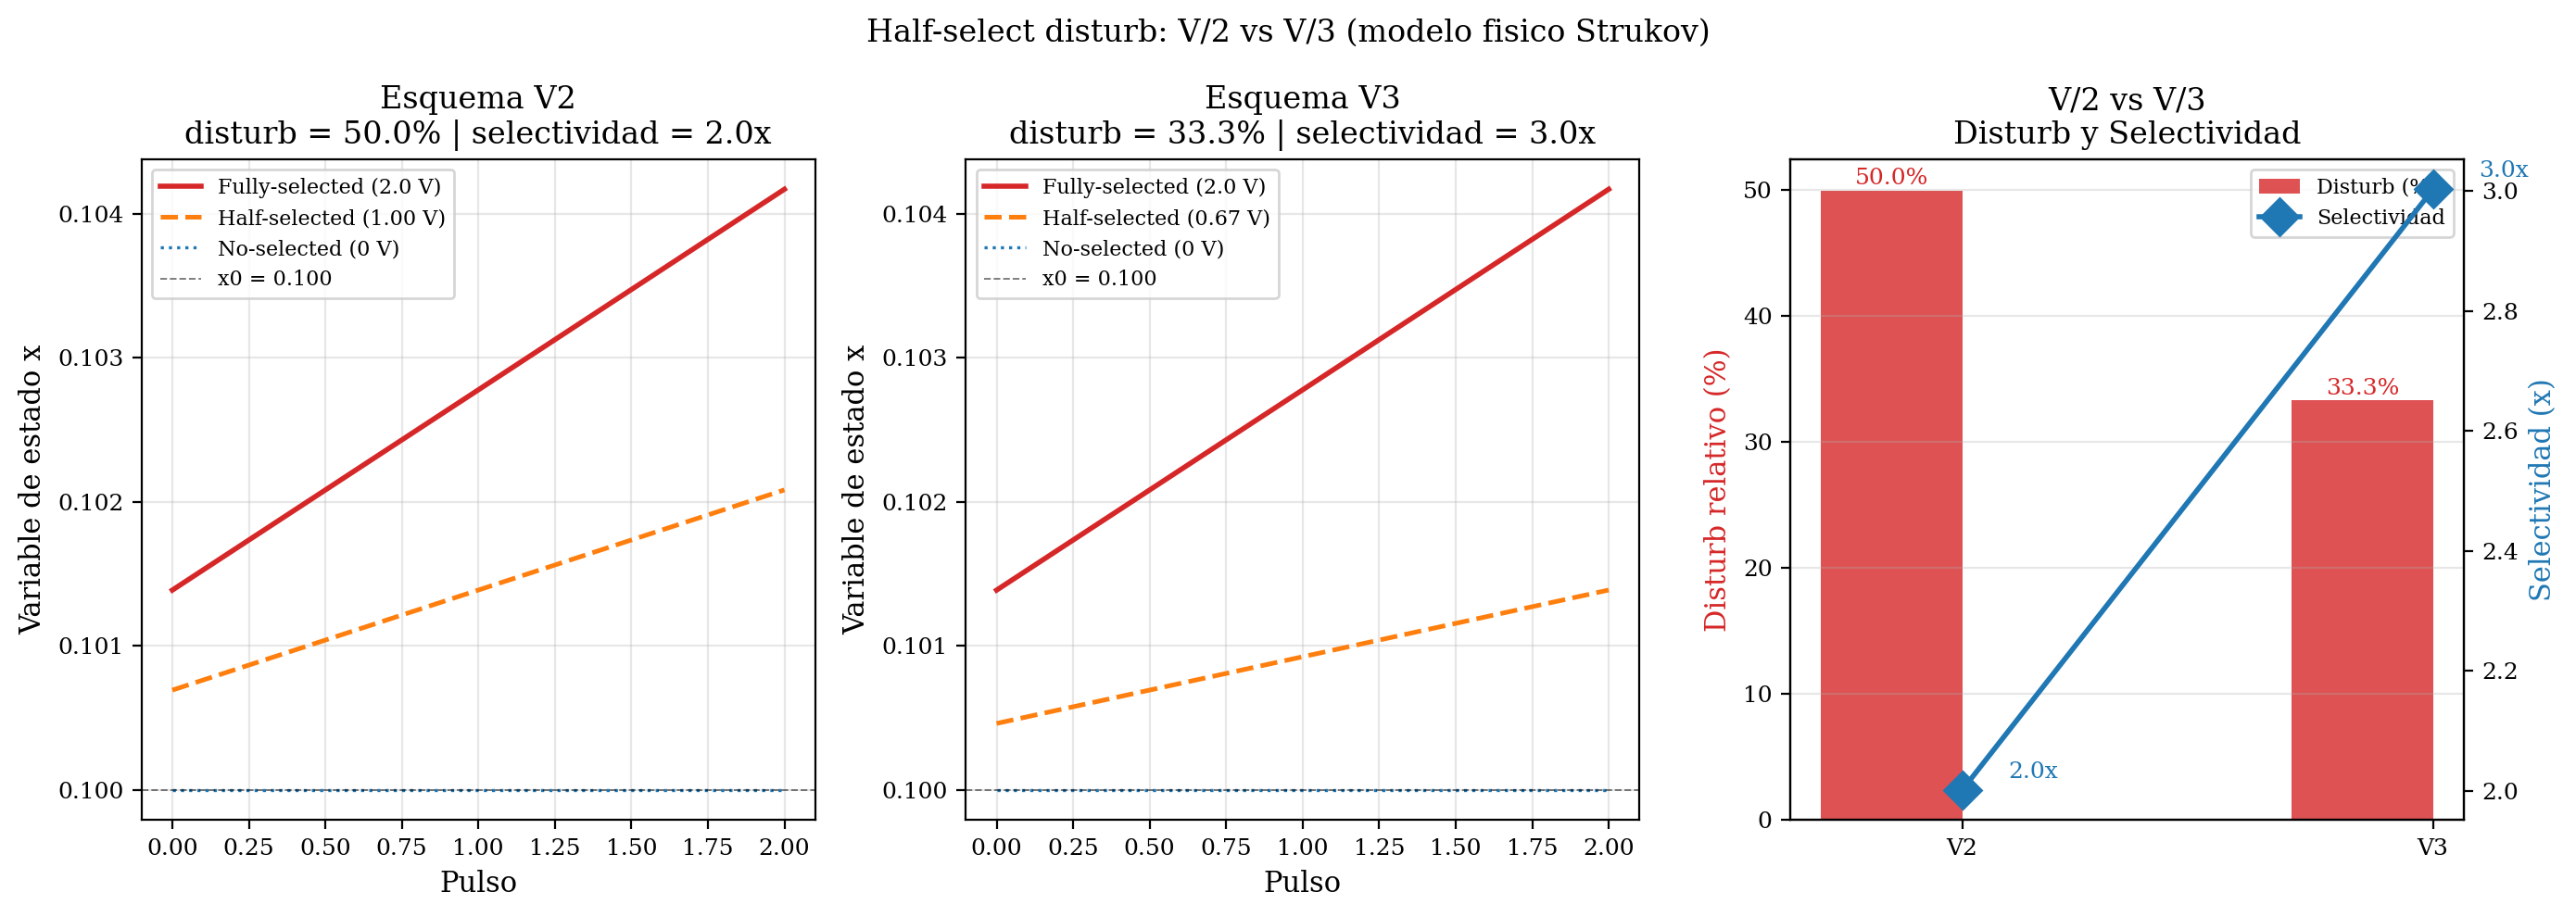
\includegraphics[width=0.95\textwidth]{experiments/figures/exp05_v2_vs_v3.png}
  \caption{Evolución de $X$ para celda fully-, half- y no-selected bajo 3 pulsos.}
  \label{fig:exp05}
\end{figure}

\paragraph{Exp.~6 --- Estado en reposo del modelo}
El resultado reportado tras 1000 pasos con $V_{\text{rows}}=0\,\text{V}$ es un cambio máximo en $X$ de $\Delta_{\max}=0$ bajo las condiciones del experimento. Esto describe el modelo y protocolo evaluados, no certifica la retención de un dispositivo físico.
\begin{figure}[H]
  \centering
  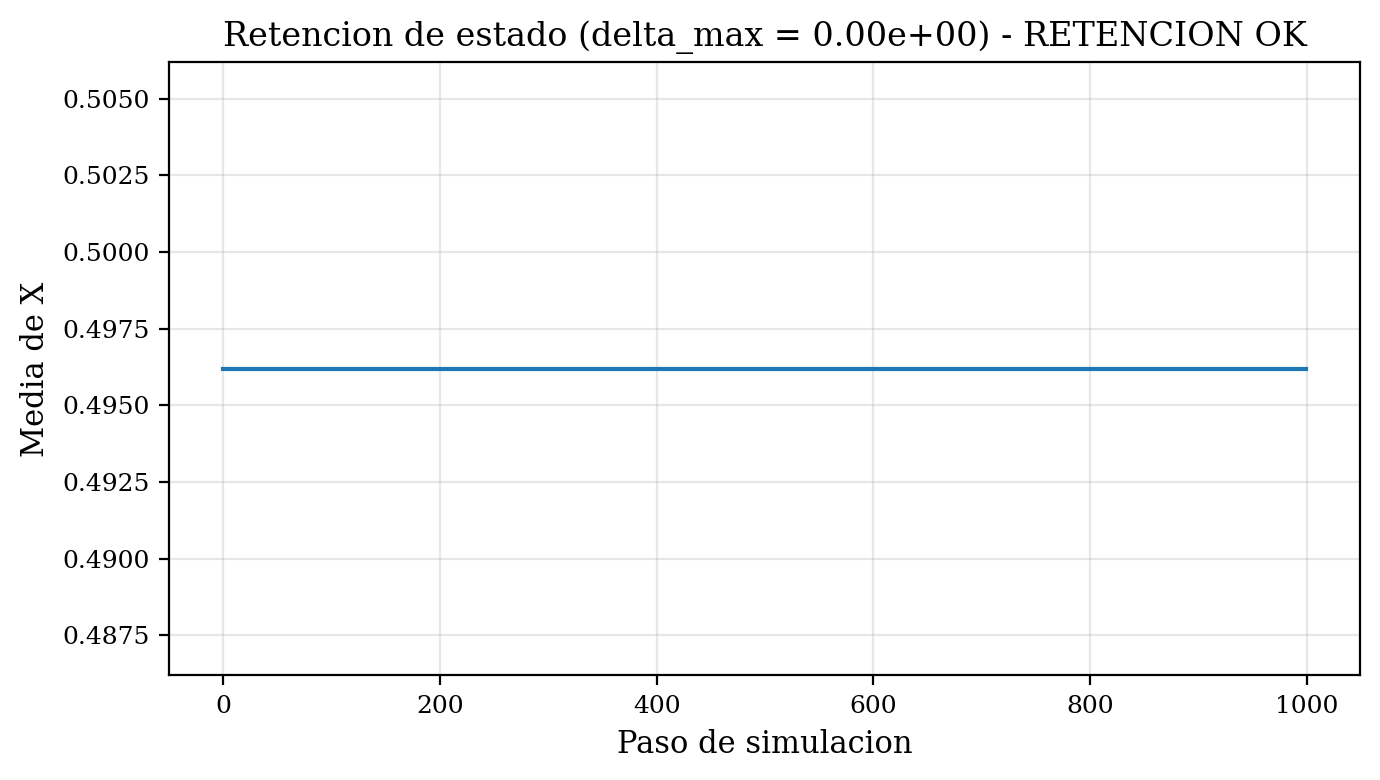
\includegraphics[width=0.62\textwidth]{experiments/figures/exp06_retention.png}
  \caption{Media de $X$ durante 1000 pasos en reposo para la simulación reportada.}
  \label{fig:exp06}
\end{figure}

\paragraph{Exp.~7 --- Respuesta simulada a pulsos LTP/LTD}
La Figura~\ref{fig:exp07} muestra la respuesta reportada del modelo bajo pulsos de potenciación (LTP, $+1\,\text{V}$) y depresión (LTD, $-1\,\text{V}$). Para 50 pulsos desde $x_0=0.1$, se reportan $x=0.135$ para LTP y $x=0.066$ para LTD. Estos valores describen la ejecución simulada y no se presentan como una respuesta experimental de un dispositivo real.
\begin{figure}[htbp]
  \centering
  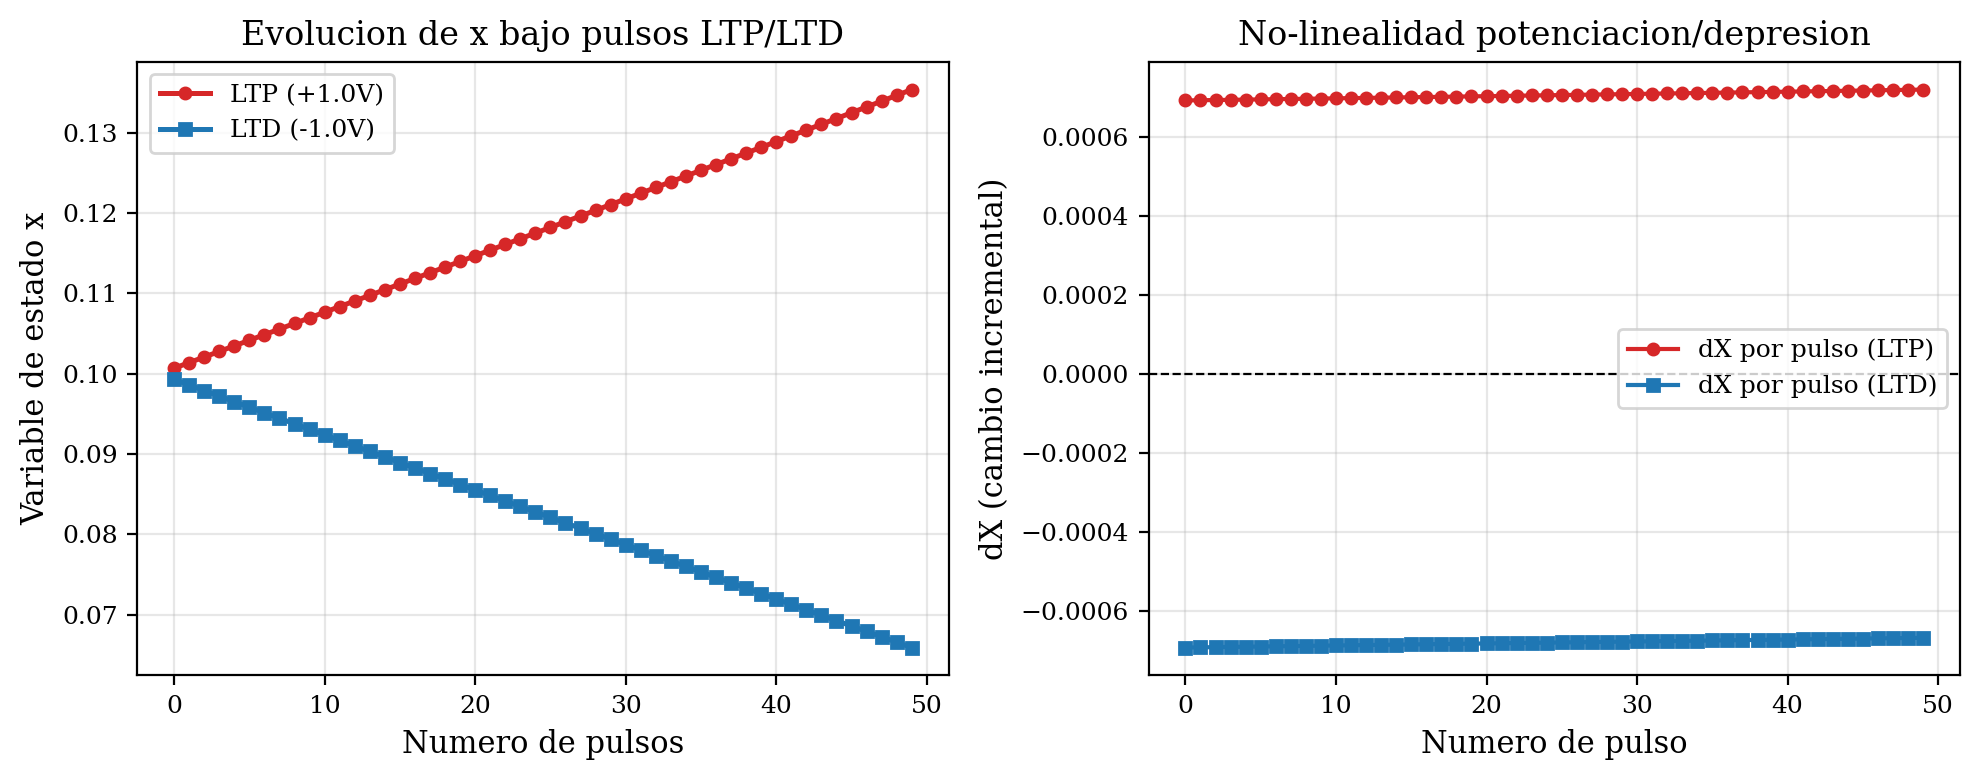
\includegraphics[width=0.88\textwidth]{experiments/figures/exp07_ltp_ltd.png}
  \caption{LTP/LTD y derivada discreta. La no-linealidad satura suavemente los extremos.}
  \label{fig:exp07}
\end{figure}

\paragraph{Exp.~8 --- Variabilidad dispositivo a dispositivo (D2D)}
La Figura~\ref{fig:exp08} cuantifica la dispersión de $I_{\text{col}}$ entre 20 crossbars virtuales. La variabilidad dispositivo-a-dispositivo se caracteriza por $CV(I_{\text{col}}) = 40.3\%$ en términos de la corriente integrada, equivalente al $4.0\%$ del rango dinámico de $\mathbf{G}$.
\begin{figure}[H]
  \centering
  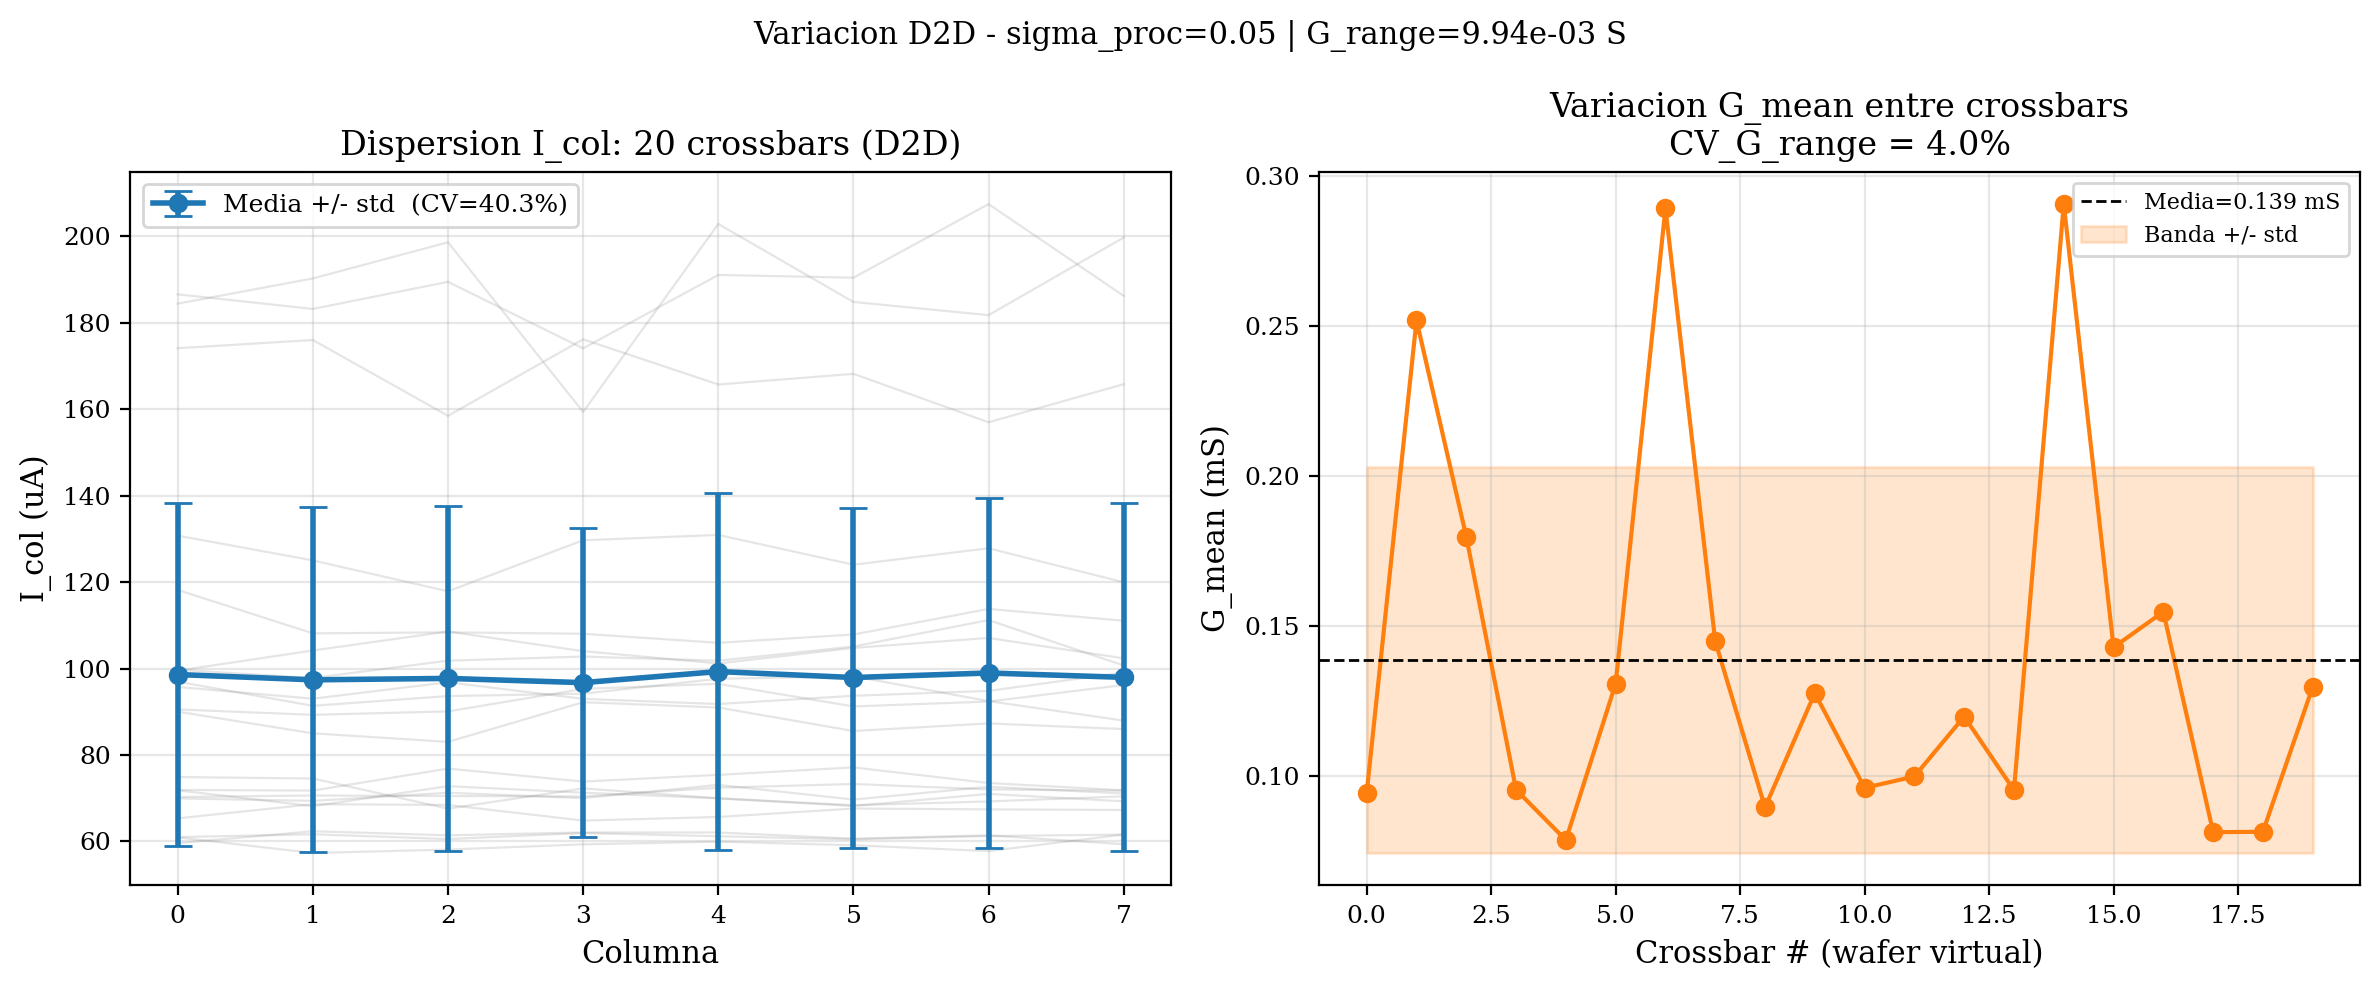
\includegraphics[width=0.88\textwidth]{experiments/figures/exp08_d2d_reproducibility.png}
  \caption{Dispersión de $I_{\text{col}}$ y variación de $\bar{G}_{\text{mean}}$ entre 20 crossbars virtuales.}
  \label{fig:exp08}
\end{figure}

\paragraph{Exp.~9 --- Costo computacional del solver MNA}
La Figura~\ref{fig:exp09} presenta un ajuste empírico reportado de
$\mathcal{O}(N^{0.85})$ y un tiempo aproximado de $\sim 3$ ms por paso para
$N=24$ en el equipo usado entonces. El exponente es propio de esa muestra y
configuración: no establece la complejidad asintótica del solver ni permite
generalizar la comparación con $\mathcal{O}(N^3)$ sin conocer el rango medido,
el hardware y el procedimiento de temporización.
\begin{figure}[H]
  \centering
  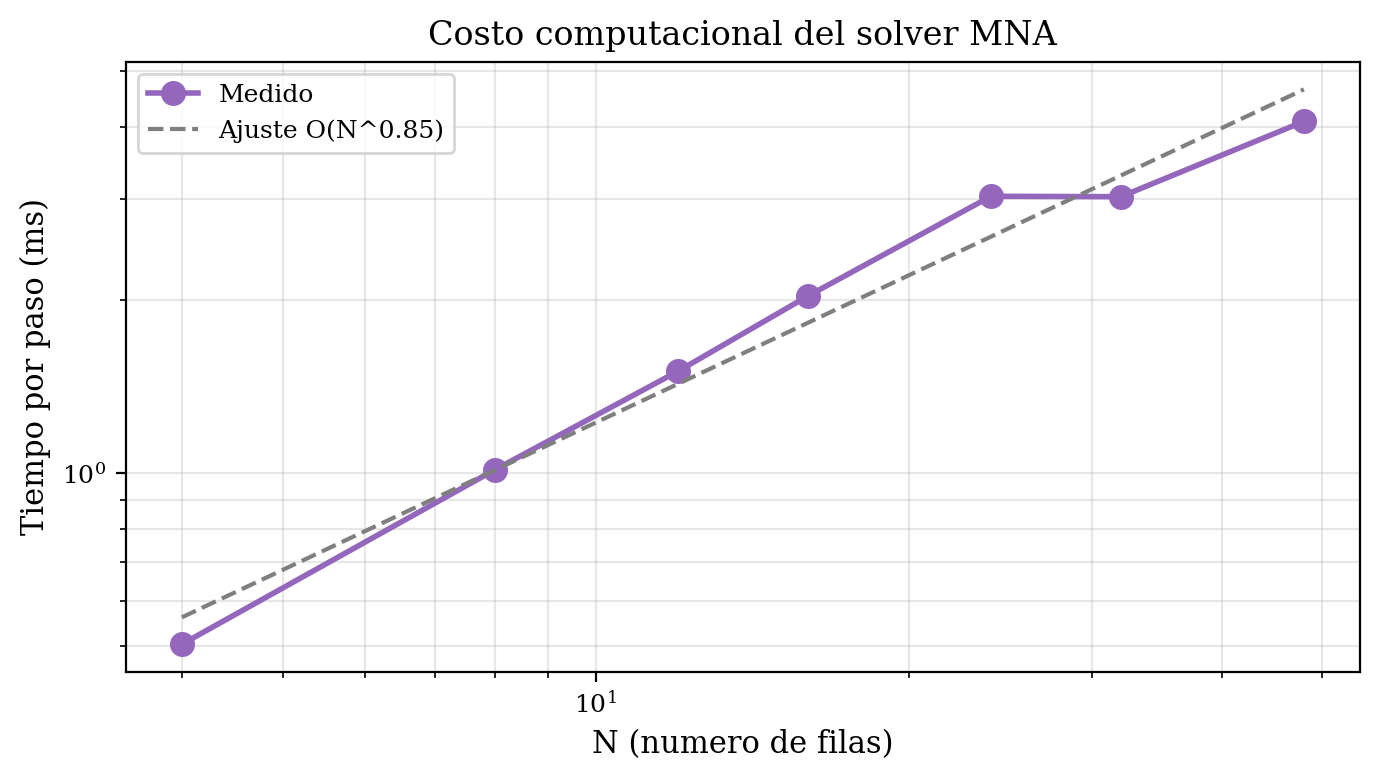
\includegraphics[width=0.62\textwidth]{experiments/figures/exp09_computational_cost.png}
  \caption{Costo computacional reportado del solver MNA en función de $N$.
El ajuste de las muestras archivadas es $\mathcal{O}(N^{0.85})$.}
  \label{fig:exp09}
\end{figure}

\paragraph{Exp.~10 --- Crosstalk entre columnas}
La Figura~\ref{fig:exp10} expone el efecto de crosstalk: al excitar únicamente la fila 0, las otras columnas muestran una desviación media del $13.32\%$ por interacción parásita MNA.
\begin{figure}[H]
  \centering
  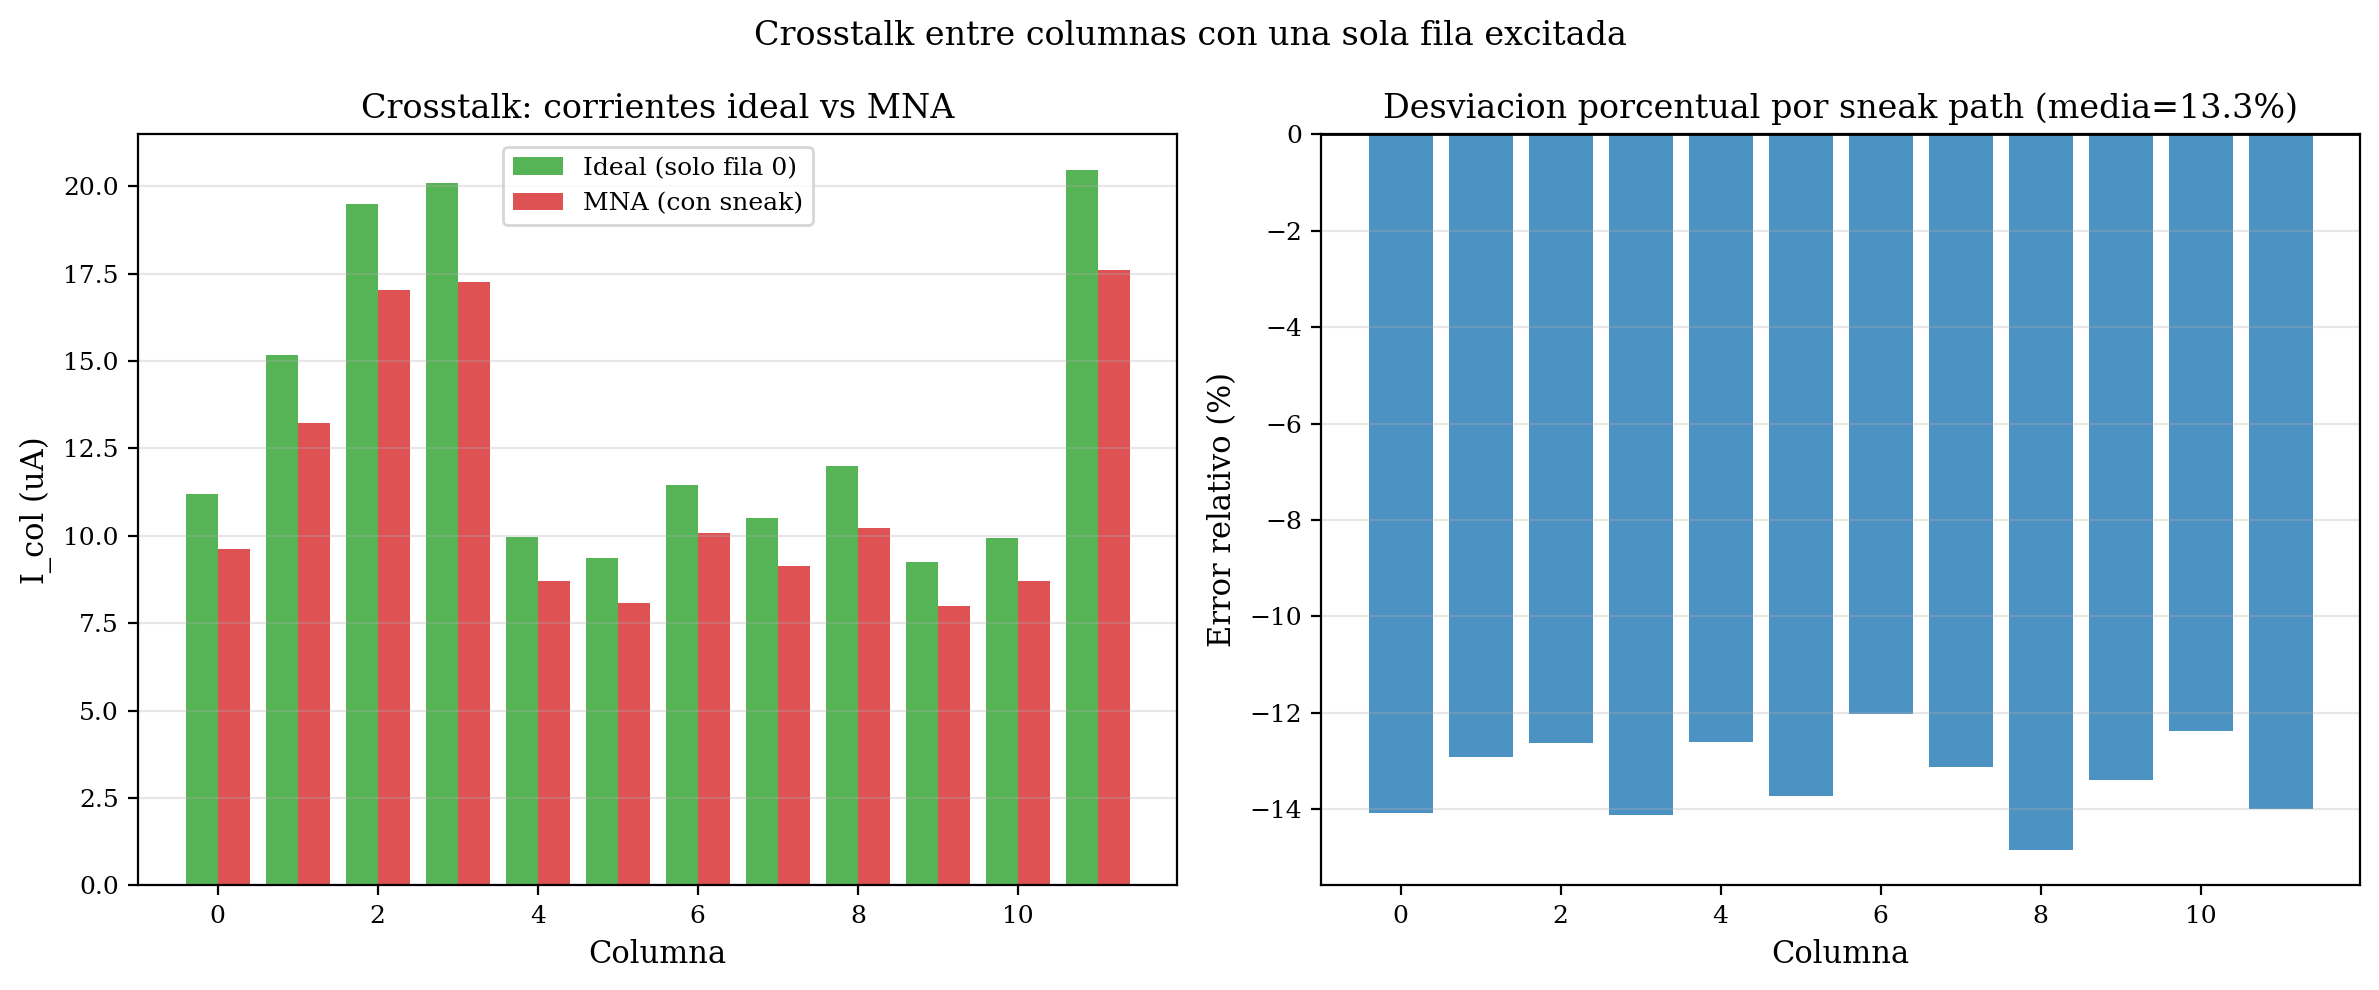
\includegraphics[width=0.88\textwidth]{experiments/figures/exp10_crosstalk.png}
  \caption{$I_{\text{col}}$ real vs.\ ideal al excitar únicamente la fila 0.}
  \label{fig:exp10}
\end{figure}

\paragraph{Alcance de los resultados de la Etapa 4}
Los diez experimentos anteriores y las figuras del agente documentan
resultados guardados de simulaciones, no mediciones de hardware. Para evitar
repetir sus cifras en un segundo resumen, esta sección deja cada resultado
junto a su configuración y figura; la tabla maestra del Apéndice C resume
únicamente las verificaciones V01--V28.

